\documentclass{article}
\usepackage{amsmath}
\usepackage{graphicx}

\begin{document}
\section{Ejecta Flux from Impact Point}\label{sec:Secondary Flux Environment}

The ejected mass from an impact is distributed at different speeds (Section \ref{sssec:Ejecta:Speed Distribution}), angles (Sections  \ref{sssec:Ejecta:Zenith Distribution} and \ref{sssec:Ejecta:Azimuth Distribution}), and sizes (Section \ref{ssec:Mass/Particle Size Distribution}). The speed and size of the ejecta is assumed to be dependent on each other -- the larger the ejected particle the slower, on average, the particle that is ejected. The impactor impact angle and azimuth determines the zenith and azimuth distribution of the ejecta. For more oblique impacts, the ejecta is projected less from normal and more towards the horizon, in addition to having a stronger component downstream with respect to the impactor azimuth in terms of the ejecta azimuth distribution. 



%%%%%%%%%%%%%%%%%%%%%%%%%%%%%%%%%%%%%%%%%%%%%%%%%%%%%%%%%%%%%%%%%%%%%%
\subsection{Ejecta Distribution}\label{ssec:Ejecta Distribution}




%%%%%%%%%%%%%%%%%%%%%%%%%%%%%%%%%%%%%%%%%%%%%%%%%%%%%%%%%%%%%%%%%%%%%%
\subsubsection{Speed Distribution}\label{sssec:Ejecta:Speed Distribution}

The speed distribution of the ejecta is determined by the scaling laws \citep{housen2011ejecta} that are assumed in this model (see Section \ref{sec:Scaling Laws}). As an approximation, the speed distribution can be described by a power-law distribution with an index that depends on the target material. However, a more complete speed distribution is used that not only includes a power-law regime, but includes proper cut-offs for the slowest speeds and fastest speeds.%, discussed in Section \ref{ssec:Min Max Ejecta Speed}.


%%%%%%%%%%%%%%%%%%%%%%%%%%%%%%%%%%%%%%%%%%%%%%%%%%%%%%%%%%%%%%%%%%%%%%
\subsubsection{Zenith Distribution}\label{sssec:Ejecta:Zenith Distribution}

\subsubsubsection{Peak Zenith Angle $\alpha_{max}$}
The ejecta zenith distribution is typically peaked at some zenith angle $\alpha_{max}$ that falls off at other angles. The peak zenith angle $\alpha_{max}$ can have different dependencies on the impactor properties.


\paragraph{Constant Zenith Peak:}
The simplest case is a constant, $\alpha_{max} = \alpha_0$, typically taken as $\alpha_0 = \pi/4$. For relatively close impact distances, an ejected angle of $45^\circ$ gives the most efficient ejecta -- the ejecta travels further for a given speed.

\paragraph{Impact Angle Dependent Zenith Peak:}
To include more information into the ejecta blanket from the impactor is to have the zenith peak as a function of the impact angle, $\alpha_{max} = \alpha_{max}(\alpha_i)$, where $\alpha_i$ is the impact angle of the impactor. For simplicity, the peak zenith angle can be taken as the downstream for all azimuth, given in Equation~\eqref{eq:peak zenith downstream}.

\paragraph{Impact Angle \& Azimuth Dependent Zenith Peak:}
An increased fidelity peak zenith angle also include information about the impactor azimuth angle, $\alpha_{max} = \alpha_{max}(\alpha_i, \beta_i)$, where $\beta_i$ is the impact azimuth.

The peak zenith angle can be modeled after experiments of oblique impacts following Figure~18 of \cite{gault1978experimental} as a proxy to the model of $\alpha_{max}$. Using a third-order polynomial for both fits to the downstream and upstream angles given in Table \ref{tab:upstream_downstream_angles}, the peak zenith angles downstream and upstream are given by
\begin{align}\label{eq:peak zenith downstream}
\alpha_{max}(\beta - \beta_i = 0) &= 0.0003\alpha_i^3 - 0.036\alpha_i^2 + 1.5206\alpha_i + 20, \text{ downstream}\\
\alpha_{max}(\beta - \beta_i = \pi) &= -0.00042\alpha_i^3 + 0.0236\alpha_i^2 + 0.129\alpha_i + 20, \text{ upstream}
\end{align}
in units of degrees, where $\beta$ is the ejecta azimuth. When both the impact and ejecta azimuth angles are in the same direction (i.e., $\beta-\beta_i = 0$), this is downstream.

\begin{table}[h]\centering
	\caption{Cone angles of upstream and downstream of impact derived from Figure 18 of \cite{gault1978experimental}.}\label{tab:upstream_downstream_angles}
	\begin{tabular}{|c | c | c |}\hline
		Impact Zenith Angle & Upstream Zenith Angle & Downstream Zenith Angle\\\hline
		0	&20	&20\\\hline
		15	&24	&35\\\hline
		30	&35	&45\\\hline
		45	&28	&40\\\hline
		60	&13	&54\\\hline
		75	&-35	&66\\\hline		
	\end{tabular}
\end{table}


\subsubsubsection{Rival \& Mandeville (Gaussian Distribution)}
One example of a peaked distribution is given in \cite{rival1999modeling}, shown below for reference:
\begin{equation}\label{eq:Rival_zenith-dist}
F(\alpha) = \frac{1}{\sigma\sqrt{2\pi}}\exp\left[-\frac{(\alpha-\alpha_{max})^2}{2\sigma^2}\right],
\end{equation}
where $\alpha_{max}$ is defined as
\begin{equation}
\alpha_{max} = 
\begin{cases}
\frac{\alpha_{max60}-\alpha_{max0}}{\pi/3}\alpha_i + \alpha_{max0}\text{  for $\alpha_i\le \pi/3 = 60^\circ$}\\
\alpha_{max60}\text{  for $\alpha_i > \pi/3 = 60^\circ$}
\end{cases},
\end{equation}
for $\alpha_i$ the impact zenith angle, and \citep[see][]{ESABASE2_DebrisRelease10.0}
\begin{align}
\alpha_{max0} &= \frac{\pi}{6} = 30^\circ,\\
\alpha_{max60} &= \frac{4\pi}{9} = 80^\circ,\\
\sigma &= \frac{\pi}{60} = 3^\circ,
\end{align}
where the peak ejecta angle is shifted from $30^\circ$ of zenith for a normal impact to $80^\circ$ of zenith for oblique impacts ($>60^\circ$).

One difficulty with this zenith distribution is the normalization, assuming ejecta is only created from $0 < \alpha < \pi/2 $. A Gaussian distribution is usually integrated from $-\infty$ to $+\infty$, so a finite integration introduces error functions.

\subsubsubsection{Raised Cosine Distribution}
A more focused zenith distribution that is easier to normalize can be described by a raised cosine distribution, given as
\begin{equation}\label{eq:zenith-rasied cosine dist}
F(\alpha) = \begin{cases}
\frac{1}{2s}\left[1 + \cos\left(\frac{\alpha-\mu}{s}\pi\right)\right] \text{, for $\mu-s \le \alpha \le \mu+s$}\\
0 \text{, otherwise}
\end{cases},
\end{equation}
This distribution is symmetric about the peak $\mu$, with a spread $s$. It is assumed that $\mu-s \ge 0$ and $\mu+s \le \pi/2$, otherwise the normalization term would be dependent on the peak, in addition to the spread.

%%%%%%%%%%%%%%%%%%%%%%%%%%%%%%%%%%%%%%%%%%%%%%%%%%%%%%%%%%%%%%%%%%%%%%
\subsubsection{Azimuth Distribution}\label{sssec:Ejecta:Azimuth Distribution}

The azimuth distribution is often dependent on the impactor azimuth such that there are more ejecta downstream for oblique impacts. Normal impacts are expected to produce a symmetric azimuth distribution. For highly oblique impacts ($\alpha_i > \pi/3$) there is often seen a \textit{butterfly pattern} \citep{shuvalov2011ejecta}. However, over a large number of oblique impacts of various sizes, it is plausible to assume that the direct downstream direction dominates the azimuth distribution.

\subsubsubsection{Rival \& Mandeville}
An example azimuth distribution can be found in \cite{rival1999modeling}, given by
\begin{equation}\label{eq:azm_rival_mandeville}
G(\beta) =
\begin{cases}
\frac{1}{2\pi}\left[1+\frac{3\alpha_i}{2\pi - 3\alpha_i}\cos(\beta-\beta_i)\right] \text{  for $\alpha_i\le \pi/3 = 60^\circ$}\\
\frac{1}{\sigma'\sqrt{2\pi}}\exp\left[-\frac{(\beta-\beta_i)^2}{2\sigma'^2}\right]
\text{  for $\alpha_i > \pi/3 = 60^\circ$}
\end{cases},
\end{equation}
where
\begin{equation}
\sigma' = \frac{\pi}{36} = 5^\circ, 
\end{equation}
for $\beta_i$ the impact azimuth angle + $\pi$.

\subsubsubsection{Variation on Rival \& Mandeville} In order to have a periodic and easy-to-normalize function, the oblique regime is modified from Equation \eqref{eq:azm_rival_mandeville} to give
\begin{equation}\label{eq:azm_mod_rival_mandeville}
G(\beta) =
\begin{cases}
\frac{1}{2\pi}\left[1+\frac{3\alpha_i}{2\pi - 3\alpha_i}\cos(\beta-\beta_i)\right] \text{  for $\alpha_i\le \pi/3 = 60^\circ$}\\
\frac{1 + \cos(\beta-\beta_i)}{2\pi}
\text{  for $\alpha_i > \pi/3 = 60^\circ$}
\end{cases}.
\end{equation}

An alteration of Equation \eqref{eq:azm_mod_rival_mandeville} on the oblique case could be to use a raised cosine distribution with a spread of $ s = 3\sigma'$.




%%%%%%%%%%%%%%%%%%%%%%%%%%%%%%%%%%%%%%%%%%%%%%%%%%%%%%%%%%%%%%%%%%%%%%
\subsection{Mass/Particle Size Distribution}\label{ssec:Mass/Particle Size Distribution}

The mass or particle size distribution of ejecta can be approximated in a few different ways. For the purpose of comparing to various sources, there are four possible ways to describe the particle size distribution, give by \citep{koschny2001impacts_mass}
\begin{align}
m_{cum}(\le d) &= k_1 d^\alpha,\label{eq:KG01 m_cum d}\\
N_{cum}(\ge m) &= k_2 m^{-\beta},\label{eq:KG01 N_cum m}\\
N_{cum}(\ge d) &= k_3 d^\gamma,\label{eq:KG01 N_cum d}\\
m_{cum}(\le m) &= k_4 m^\delta,\label{eq:KG01 m_cum m}
\end{align}
with $N_{cum}$ the cumulative number, $m_{cum}$ the cumulative mass, $d$ the particle diameter, and $m$ the particle mass.

The various transformations between the four possible descriptions are:
\begin{align}
\beta &= -\gamma/3,\\
\alpha &= 3(1-\beta),\\
\alpha &= \gamma + 3,\\
\delta &= \alpha/3.
\end{align}

Table IV of \citep{koschny2001impacts_mass} gives examples of the exponent $\alpha$, summarized here in Table \ref{tab:mass-diameter_index_examples}.

\begin{table}[!htb]
	\begin{center}
	\caption{A compilation of indices of the various particle size distribution descriptions. Values that are in bold are the index that was originally used in the corresponding source.}\label{tab:mass-diameter_index_examples}
	\begin{tabular}{|c | c | c | c | c|}\hline
		\textbf{Target Material} & \textbf{Source} & $\alpha$ & $\beta$ & $-\gamma$ \\\hline
		Basalt	& \cite{koschny2001impacts_mass}	& \textbf{0.56, 0.96} & 0.81, 0.68 & 2.44, 2.04\\\hline
		Granite	& ''	&\textbf{ 0.44} & 0.85 & 2.56\\\hline
		Gabbro	& ''	& \textbf{1.41} & 0.53 & 1.59\\\hline
		Alumina	& ''	& \textbf{1.08} & 0.64 & 1.92\\\hline
		Water ice	& ''	& \textbf{1.3} & 0.57 & 1.7\\\hline
		Porous ice-silicate	& ''	& \textbf{1.8} & 0.4 & 1.2\\\hline
		Compact ice-silicate	& ''	& \textbf{1.4$\pm$0.3} & 0.53$\pm$0.1 & 1.6$\pm$0.3\\\hline
		Basalt & \cite{cour1969meteoroid} & -0.6 & \textbf{1.2} & 3.6\\\hline
		Sandstone & \cite{buhl2014ejecta} & 0.26-0.46 & 0.85-0.91 & \textbf{2.54-2.74} \\\hline
		Apollo Samples & \cite{carrier2003particle} & -0.55 & 1.18 & \textbf{3.55}$^a$ \\\hline
		Basalt + others & \cite{oKeefe1985impact} & \textbf{0.42-0.53} & 0.82-0.86 & 2.47-2.58 \\\hline
		\multicolumn{5}{l}{\footnotesize $^a$ valid for diameters from $10^{-6}$ m to $10^{-1}$ m.}
	\end{tabular}
\end{center}
\end{table}


\subsubsection{NASA SP-8013}
The Meteoroid Environment Model - 1969 Near Earth to Lunar Surface \citep{cour1969meteoroid}, or NASA SP-8013, contains both the primary meteoroid environment as well as the lunar ejecta environment. The latter is given in terms of cumulative number flux of secondary ejecta greater than mass $m$ (i.e., in the form of Equation \eqref{eq:KG01 N_cum m}), shown in Figure \ref{fig:NASA-SP-8013-Fig10-flux-mass-distribution} (Figure 10 of \cite{cour1969meteoroid}).


\begin{figure}[!htb]
	\centering
	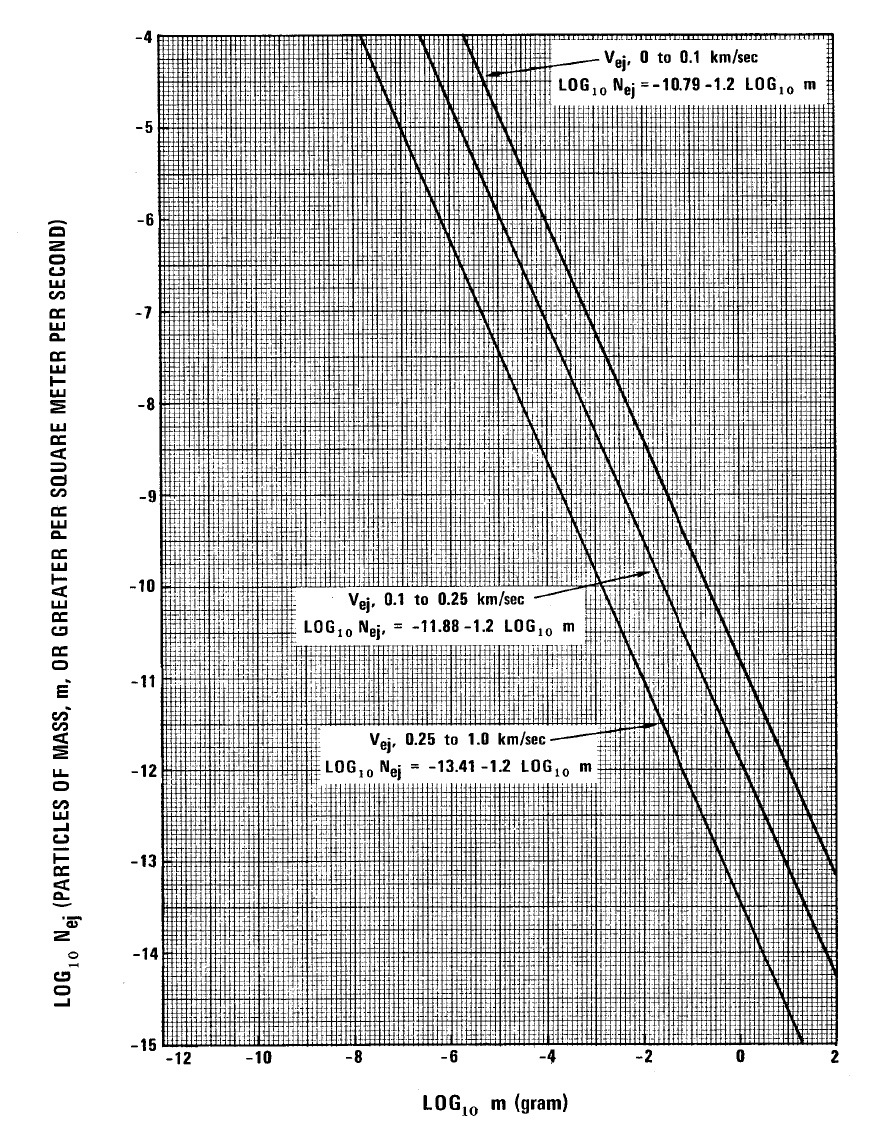
\includegraphics[width=1.0\linewidth]{NASA-SP-8013-Fig10-flux-mass-distribution.PNG}
	\caption{Average cumulative lunar ejecta flux-mass distribution for each of three ejecta velocity intervals \citep{cour1969meteoroid}.}\label{fig:NASA-SP-8013-Fig10-flux-mass-distribution}
\end{figure}

Each of the three velocity intervals have a power-law index of $-\beta = -1.2$, corresponding to $\alpha=-0.6$ (see Table \ref{tab:mass-diameter_index_examples}). Qualitatively, the larger the power-law index $\alpha$ is, the greater number of larger particles are present in the size distribution \citep[e.g.,][]{koschny2001impacts_mass,bierhaus2018secondary}. For a negative $\alpha$, this implies an absence of larger sized particles in the SP-8013 model compared to what is shown in \cite{koschny2001impacts_mass}.

The power-law index of $-\beta = -1.2$ is a simplification of \cite{zook1967problem}, which is what the SP-8013 is based on for lunar ejecta. Figure 5 of \cite{zook1967problem} displays three different velocity ranges with $\beta = 1$ for $0 \le v \le 100$ m/s, $\beta = 1$ for $100 \le v \le 250$ m/s, and $\beta = 1.16$ for $250 \le v \le 1000$ m/s.

It is interesting to point out that the particle size distribution shown in Figure \ref{fig:NASA-SP-8013-Fig10-flux-mass-distribution} has a similar power-law index with the regolith particle size distribution of diameters from $10^{-6}$ m to $10^{-1}$ m of \cite{carrier2003particle}, see Table \ref{tab:mass-diameter_index_examples}. Since the regolith particle size distribution is a log-normal distribution, the power-law index for larger diameters will be even more steep, and therefore a more negative $\alpha$, meaning there is an absence of larger stones or boulders in the top layers of regolith sampled from Apollo.

\subsubsection{O'Keefe \& Ahrens 1985}\label{sssec:OKeefe Ahrens 1985}
A conclusion from \cite{sachse2015correlation} states that \textit{the assumption that the size of the fragments and the speed at the moment of ejection are uncorrelated} should be dropped. In practice, larger ejected particles typically have slower speeds while smaller ejected particles have faster speeds. This observation is not seen in the previous size distribution model of NASA SP-8013\footnote{It is important to note that \cite{zook1967problem} did include a speed dependent size distribution in their model (they looked at three variations, ultimately using a piece-wise power-law model), however, \cite{cour1969meteoroid} in SP-8013 simplified the size distribution to be constant for each of the speed ranges.}, so another model is sought after.

The particle size distribution discussed in \cite{oKeefe1985impact} gives a way to introduce a speed-dependent particle size distribution. The cumulative amount of mass of ejecta fragments of mass greater than $m$ is given by (Equation (11) of \cite{oKeefe1985impact}), note $\beta_{OK85} \equiv \alpha$ as in Table \ref{tab:mass-diameter_index_examples},
\begin{equation}\label{eq:f(m,mbv)}
f(m, m_{bv}(v)) = 1 - \left(\frac{m}{m_{bv}}\right)^{\frac{\beta_{OK85}}{3}},
\end{equation}
where the mass of the largest fragment ejected at a given ejected velocity $v$ is
\begin{equation}
\frac{m_{bv}(v)}{m_b} = \left(\frac{v}{v_{min}}\right)^{-\delta_{OK85}}.
\end{equation}
The speed index $\delta_{OK85}$ is related to the power-law index of the CDF of mass exceeding a certain speed of ejecta (e.g., $3\mu$ from \cite{housen2011ejecta}) and the CDF of mass not exceeding a certain diameter, i.e.\ $\alpha$, given by
\begin{equation}
\delta_{OK85} = \frac{9\mu}{\alpha}.
\end{equation}

The minimum velocity $v_{min}$ is defined as the minimum speed at which an ejected particle can reach the rim of a crater from the bottom of the crater,
\begin{equation}
v_{min} = 2\sqrt{\frac{gR}{K}},
\end{equation}
where $g$ is the lunar gravitational constant, $R$ is the crater radius (see Section \ref{ssec:Crater Size}), and $K$ is the crater diameter-to-depth ration which typically varies between $5$ and $20$. 

The maximum fragmentation mass is given in \cite{oKeefe1985impact} as
\begin{equation}
m_b = 0.2 M_{tot}^{0.8},
\end{equation}
where $M_{tot}$ is the total mass ejected from the crater by an impactor in grams, see Section \ref{ssec:Mass Ejected from Crater}. On the other hand, \cite{koschny2001impacts_mass} have a more conservative estimate on the maximum fragmentation mass with
\begin{equation}
m_b = 0.01 M_{tot}.
\end{equation}


%%%%%%%%%%%%%%%%%%%%%%%%%%%%%%%%%%%%%%%%%%%%%%%%%%%%%%%%%%%%%%%%%%%%%%
\subsubsection{Mass Distribution with Speed Distribution Weighting}\label{sssec:Mass Distribution with Speed Distribution Weighting}
Starting with the definition described by \cite{oKeefe1985impact} of the cumulative ejecta mass distribution as a function of the ejecta speed $f(m, m_{bv}(v))$ (Equation~\eqref{eq:f(m,mbv)}), the ejecta mass distribution is found by taking the derivative with respect to the mass,
\begin{equation}\label{eq:df(m,mbv)}
-\frac{df(m, m_{bv}(v))}{dm} = \frac{\beta}{3m_{bv}}\left(\frac{m}{m_{bv}}\right)^{\frac{\beta}{3}-1}.
\end{equation}
The complete ejecta mass distribution for a given impact is computed by taking the ejecta mass distribution for a given ejecta speed (Equation~\eqref{eq:df(m,mbv)}) and convoluting it with the ejected mass per speed (i.e., the speed distribution, Equation~\eqref{eq:v/U}),
\begin{equation}
f_{\mathcal{C}}(m_{ej}) = -\int_{v_{min}}^{v_{max}(m_{ej})}
dv\frac{df}{dm}\frac{dM}{dv},
\end{equation}
where the upper limit is (specifying $m_{ej}$ as the ejecta mass as opposed to the impactor mass $m_{imp}$)
\begin{equation}
v_{max}(m_{ej}) = \min\left[v_{min}(m_{ej}/m_b)^{-1/\delta}, v_{max}\right],
\end{equation}
and making the change of variables to the location from the center of the crater $x$ from the speed $v$, (note, $x = n_2 R y$)
\begin{align} % https://www.physicsread.com/latex-big-brackets/
f_{\mathcal{C}}(m) &= \int^{x(v_{min})}_{x(v_{max}(m))}
dx\frac{df}{dm}\frac{dM}{dx},\\\nonumber
&= A_\mathcal{C}\left(\frac{m_{ej}}{m_b}\right)^{\frac{\beta}{3}-1}
\int^{\frac{x(v_{min})}{n_2 R}}_{\frac{x(v_{max}(m))}{n_2 R}}
dy y ^{-\frac{\beta\delta}{3\mu}+2}(1-y)^{\frac{\beta\delta p}{3}},\\
&= A_\mathcal{C}\left(\frac{m_{ej}}{m_b}\right)^{\frac{\beta}{3}-1}
\Biggl\{
\beta\left[\frac{x(v_{min})}{n_2 R}; -\frac{\beta\delta}{3\mu}+3, \frac{\beta\delta p}{3} + 1\right]\\\nonumber
& - \beta\left[\frac{x(v_{max}(m_{ej}))}{n_2 R}; -\frac{\beta\delta}{3\mu}+3, \frac{\beta\delta p}{3} + 1\right]
\Biggr\},
\end{align}
where the constants with respect to $m_{ej}$ are
\begin{equation}
A_\mathcal{C} = \frac{3k\beta}{4\pi}\frac{m_{imp}}{m_b}
\left(\frac{\rho}{\delta}\right)^{-\frac{\beta\delta\nu}{\mu}+1}
\left(\frac{C_1 U}{v_{min}}\right)^{\frac{\beta\delta}{3}}
\left(\frac{a}{n_2 R}\right)^{\frac{\beta\delta}{3\mu}-3},
\end{equation}
with $\beta(z; a, b)$ as the incomplete beta function, $a$ is the projectile radius, $R$ is the crater radius (Equation \eqref{eq:R gravity} or \eqref{eq:R strength}), and the scaling law parameters $n_1$, $n_2$, $p$, $\mu$, $\nu$, $k$, and $C_1$ are found in Table \ref{tab:scaling law parameters}. Additional constants $\beta$ and $\delta$ can be found in Section \ref{sssec:OKeefe Ahrens 1985}.




%%%%%%%%%%%%%%%%%%%%%%%%%%%%%%%%%%%%%%%%%%%%%%%%%%%%%%%%%%%%%%%%%%%%%%
\subsection{Total Kinetic Energy}\label{ssec:Total Kinetic Energy}

The kinetic energy of the impactor gets converted into many forms during the cratering process; heat, light, compression, phase changing, and kinetic energy to the ejecta. In this section, the total energy imparted to the ejecta is computed.

The total kinetic energy of the ejecta $E_{tot,ej}$ can be calculated by taking the second moment of the ejecta mass distribution as
\begin{equation}
E_{tot,ej} = \frac{1}{2}\int_{0}^{v_{max}}dv \left(-\frac{dM}{dv}\right)v^2,
\end{equation}
where the ejecta mass distribution $dM/dv$ is defined as Equation \eqref{eq:dM/dv chain rule} and explicitly given in Equation \eqref{eq:dM/dv final}, and the ejecta speed $v$ in terms of the crater parameters (Equation~\eqref{eq:v/U}).

Changing variables from ejecta speed $v$ to location in the crater $x$, the total ejecta kinetic energy is\footnote{Note, $\beta(1-x; b, a) = \beta(1; a, b) - \beta(x; a, b)$.}
\begin{align}
E_{tot,ej} &= \frac{1}{2}\int_{n_2 R}^{n_1 a}dx \left(-\frac{dM}{dx}\right)v(x)^2,\\\nonumber
&= \frac{3}{2}M_{tot}v_{max}^2\frac{\left(1-\frac{n_1 a}{n_2 R}\right)^{-2p}}{1-\left(\frac{n_1 a}{n_2 R}\right)^3}
\int_{n_1 a}^{n_2 R}
\frac{dx}{n_2 R}\left(\frac{x}{n_1 a}\right)^{-\frac{2}{\mu}}\left(\frac{x}{n_2 R}\right)^2\left(1-\frac{x}{n_2 R}\right)^{2p},\\\nonumber
& = \frac{3}{2}M_{tot}v_{max}^2\frac{\left(1-\frac{n_1 a}{n_2 R}\right)^{-2p}\left(\frac{n_1 a}{n_2 R}\right)^{\frac{2}{\mu}}}{1-\left(\frac{n_1 a}{n_2 R}\right)^3}
\beta\left(\frac{x}{n_2 R}; -\frac{2}{\mu}+3, 2p+1\right)\bigg\rvert^{x=n_2 R}_{x=n_1 a},\\
&=\frac{3}{2}M_{tot}v_{max}^2\frac{\left(1-\frac{n_1 a}{n_2 R}\right)^{-2p}\left(\frac{n_1 a}{n_2 R}\right)^{\frac{2}{\mu}}}{1-\left(\frac{n_1 a}{n_2 R}\right)^3}
\beta\left(1-\frac{n_1 a}{n_2 R}; 2p+1, -\frac{2}{\mu}+3\right),
\end{align}
where $M_{tot}$ is the total mass ejected from the crater (Equation \eqref{eq:Mtot}), $v_{max}$ is the maximum ejecta speed for the particular crater (Equation \eqref{eq:vmax}), $a$ is the projectile radius, $R$ is the crater radius (Equation \eqref{eq:R gravity} or \eqref{eq:R strength}), and the scaling law parameters $n_1$, $n_2$, $p$, $\mu$, $\nu$, $k$, and $C_1$ are found in Table \ref{tab:scaling law parameters}. Also note, $\beta(z; a, b)$ is the incomplete beta function\footnote{\href{https://functions.wolfram.com/GammaBetaErf/Beta3/}{https://functions.wolfram.com/GammaBetaErf/Beta3/}}\textsuperscript{,}\footnote{Do not use the regularized incomplete beta function implementations. Use the Gauss hypergeometric function $_2F_1$ representation instead to avoid issues when the second parameter is a negative integer.}.
The total ejecta energy can also be written in terms of the impactor mass $m$ and normal component of the impactor speed $U$ 
\begin{equation}\label{eq:Etotej}
E_{tot,ej} = \frac{9kC_1^2}{8\pi}\left(\frac{\rho}{\delta}\right)^{-\frac{2\nu}{\mu}+1}\left(\frac{a}{n_2 R}\right)^{\frac{2}{\mu}-3}
\beta\left(1-\frac{n_1 a}{n_2 R}; 2p+1, -\frac{2}{\mu}+3\right)
mU^2,
\end{equation}
where $\rho$ is the target bulk density and $\delta$ is the impactor density.

An example of Equation \eqref{eq:Etotej} is shown in Figures \ref{fig:TotalEjectaKE_vs_EffectiveCraterSize} and \ref{fig:TotalEjectaKE_vs_EffectiveCraterSize_WCB}. The effect of the choice of surrogate material for the regolith can be seen in the differences between these two figures. The Weakly cemented basalt in Figure \ref{fig:TotalEjectaKE_vs_EffectiveCraterSize_WCB} compared with the sand fly ash in Figure \ref{fig:TotalEjectaKE_vs_EffectiveCraterSize} has about a factor of $8$ less kinetic energy transferred from the impactor to the ejected material. The work of \cite{hartmann1985impact} (Table II) provides experimental estimates of the estimated fraction of impact energy in ejecta.


\begin{figure}[!htb]
	\centering
	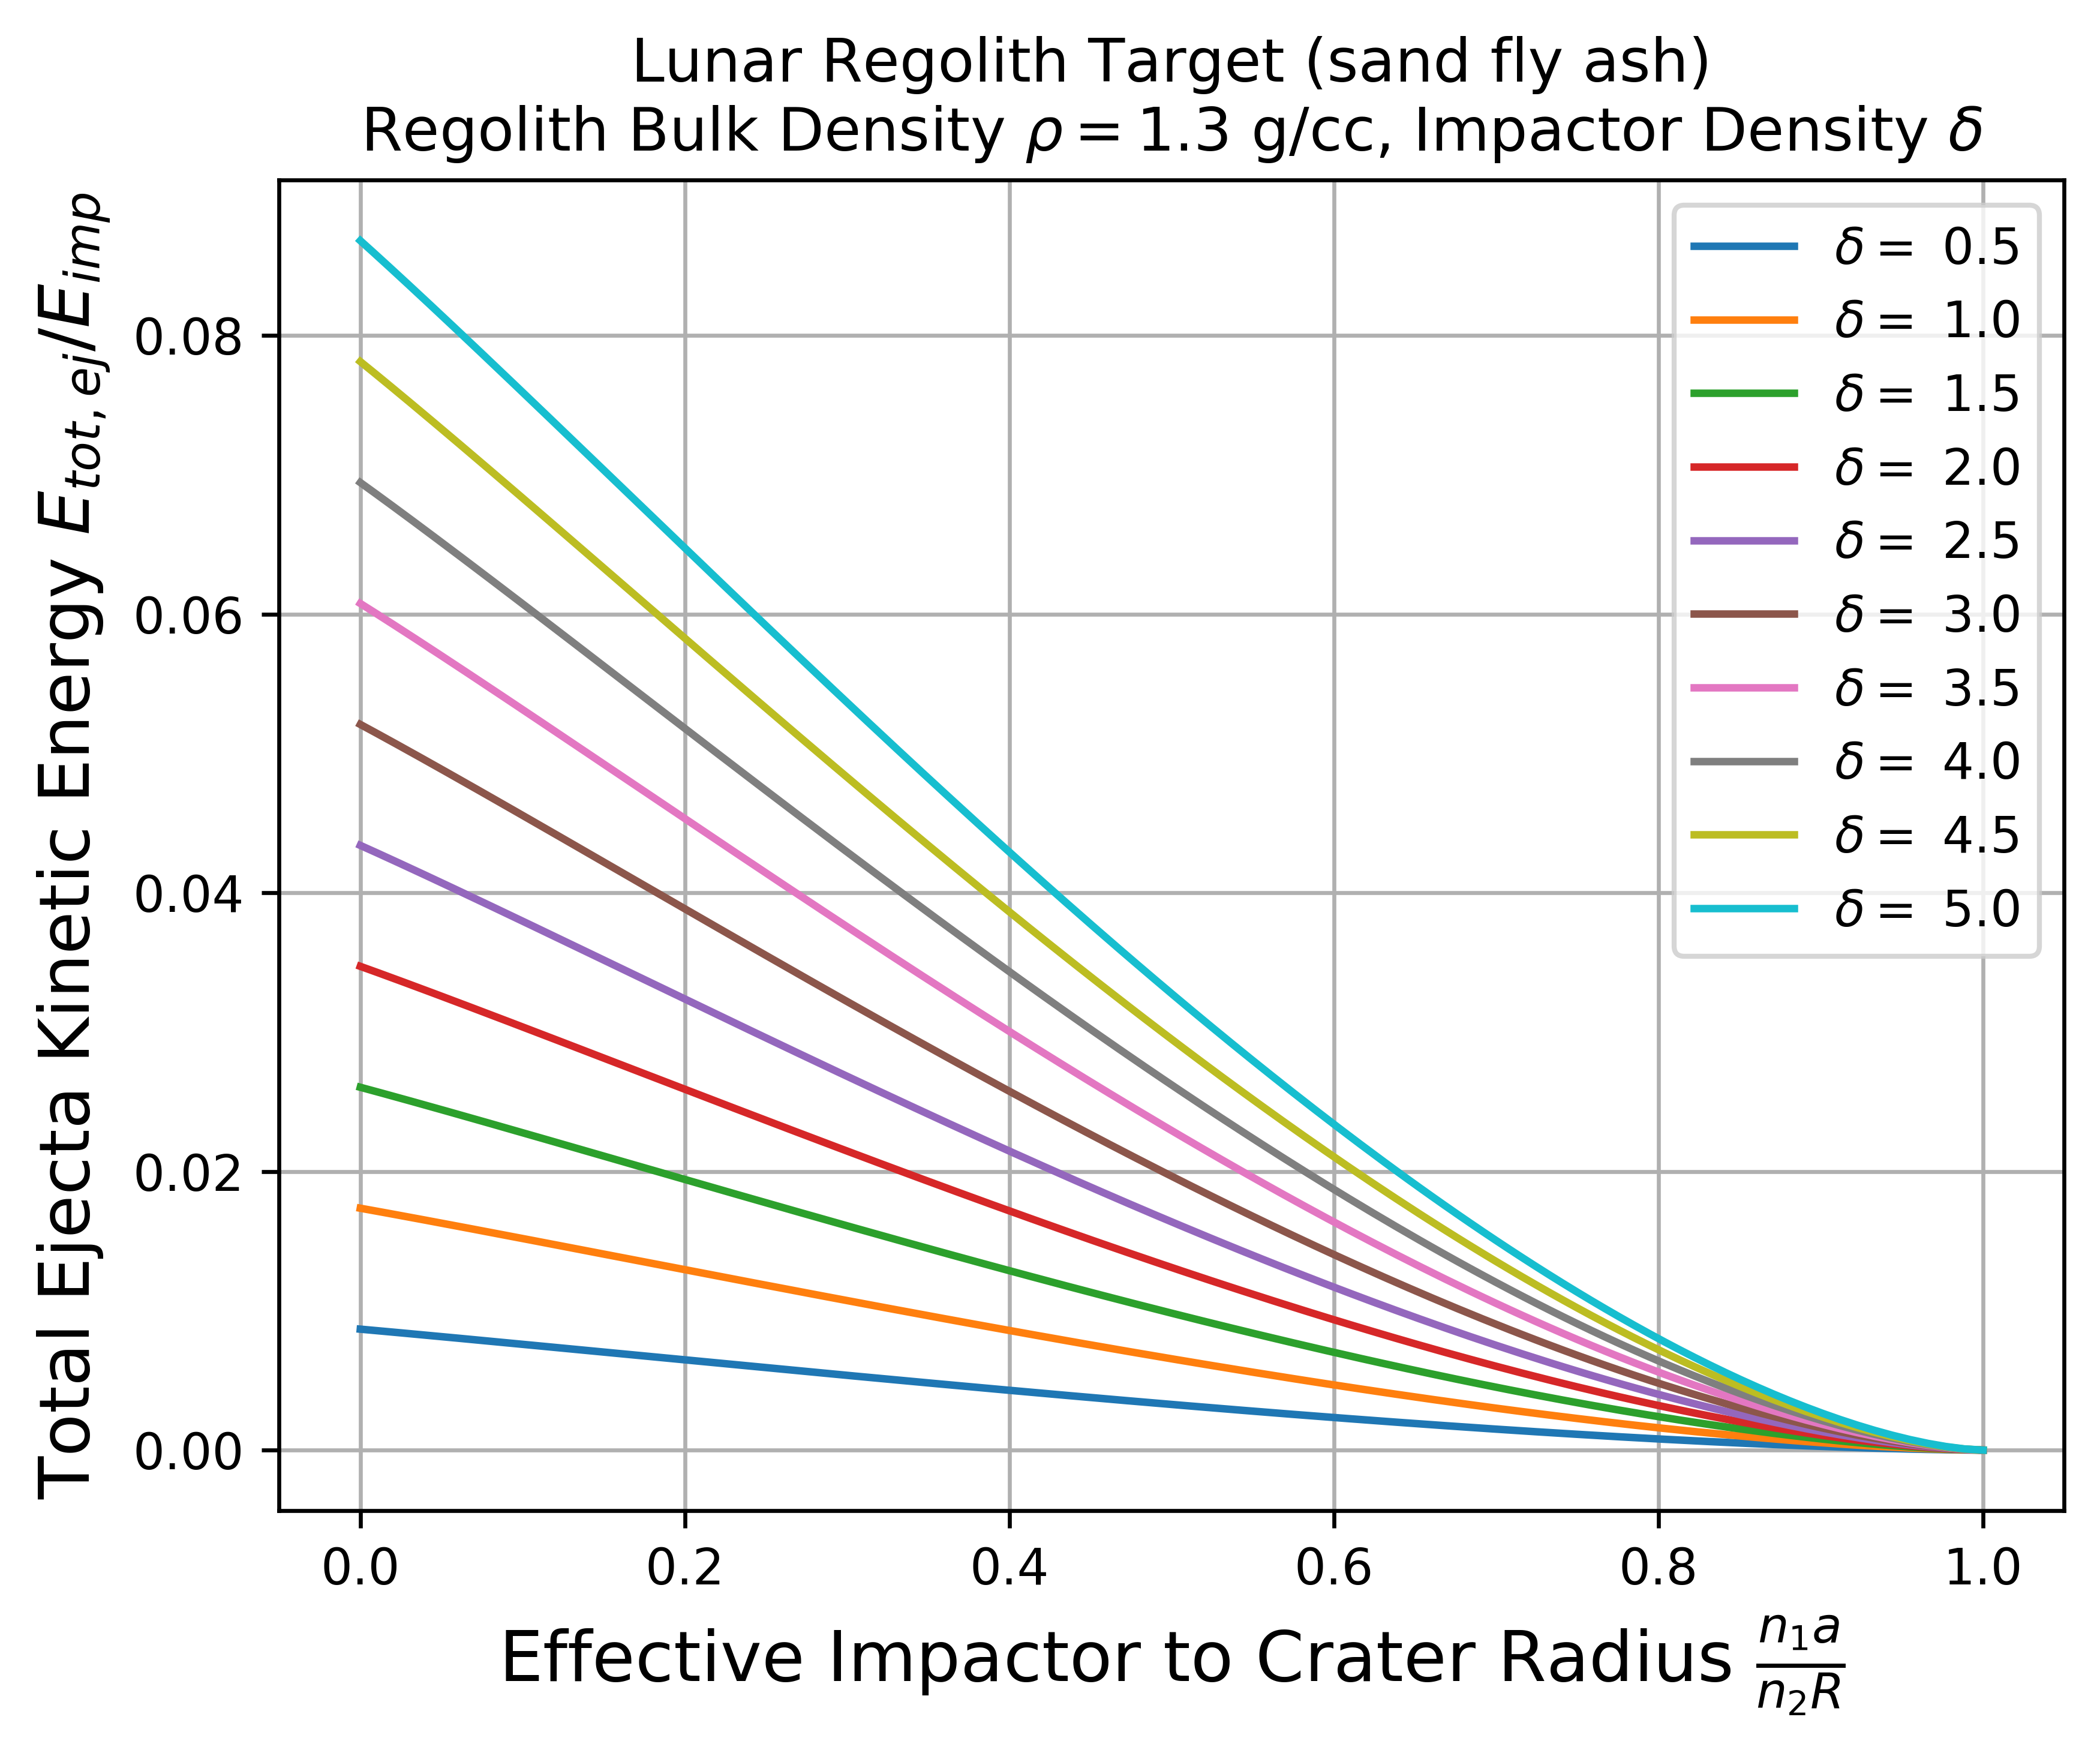
\includegraphics[width=0.65\linewidth]{TotalEjectaKE_vs_EffectiveCraterSize.png}
	\caption{The total ejecta kinetic energy $E_{tot,ej}$ (Equation \eqref{eq:Etotej}) over impactor energy $E_{imp} = \frac{1}{2}mU^2$ vs.\ effective impactor to crater radius $\frac{n_1 a}{n_2 R}$ for a lunar regolith target (using SFA in Table~\ref{tab:scaling law parameters}) with regolith surface bulk density $\rho = 1.3$ g/cc and varying impactor densities. }\label{fig:TotalEjectaKE_vs_EffectiveCraterSize}
\end{figure}

\begin{figure}[!htb]
	\centering
	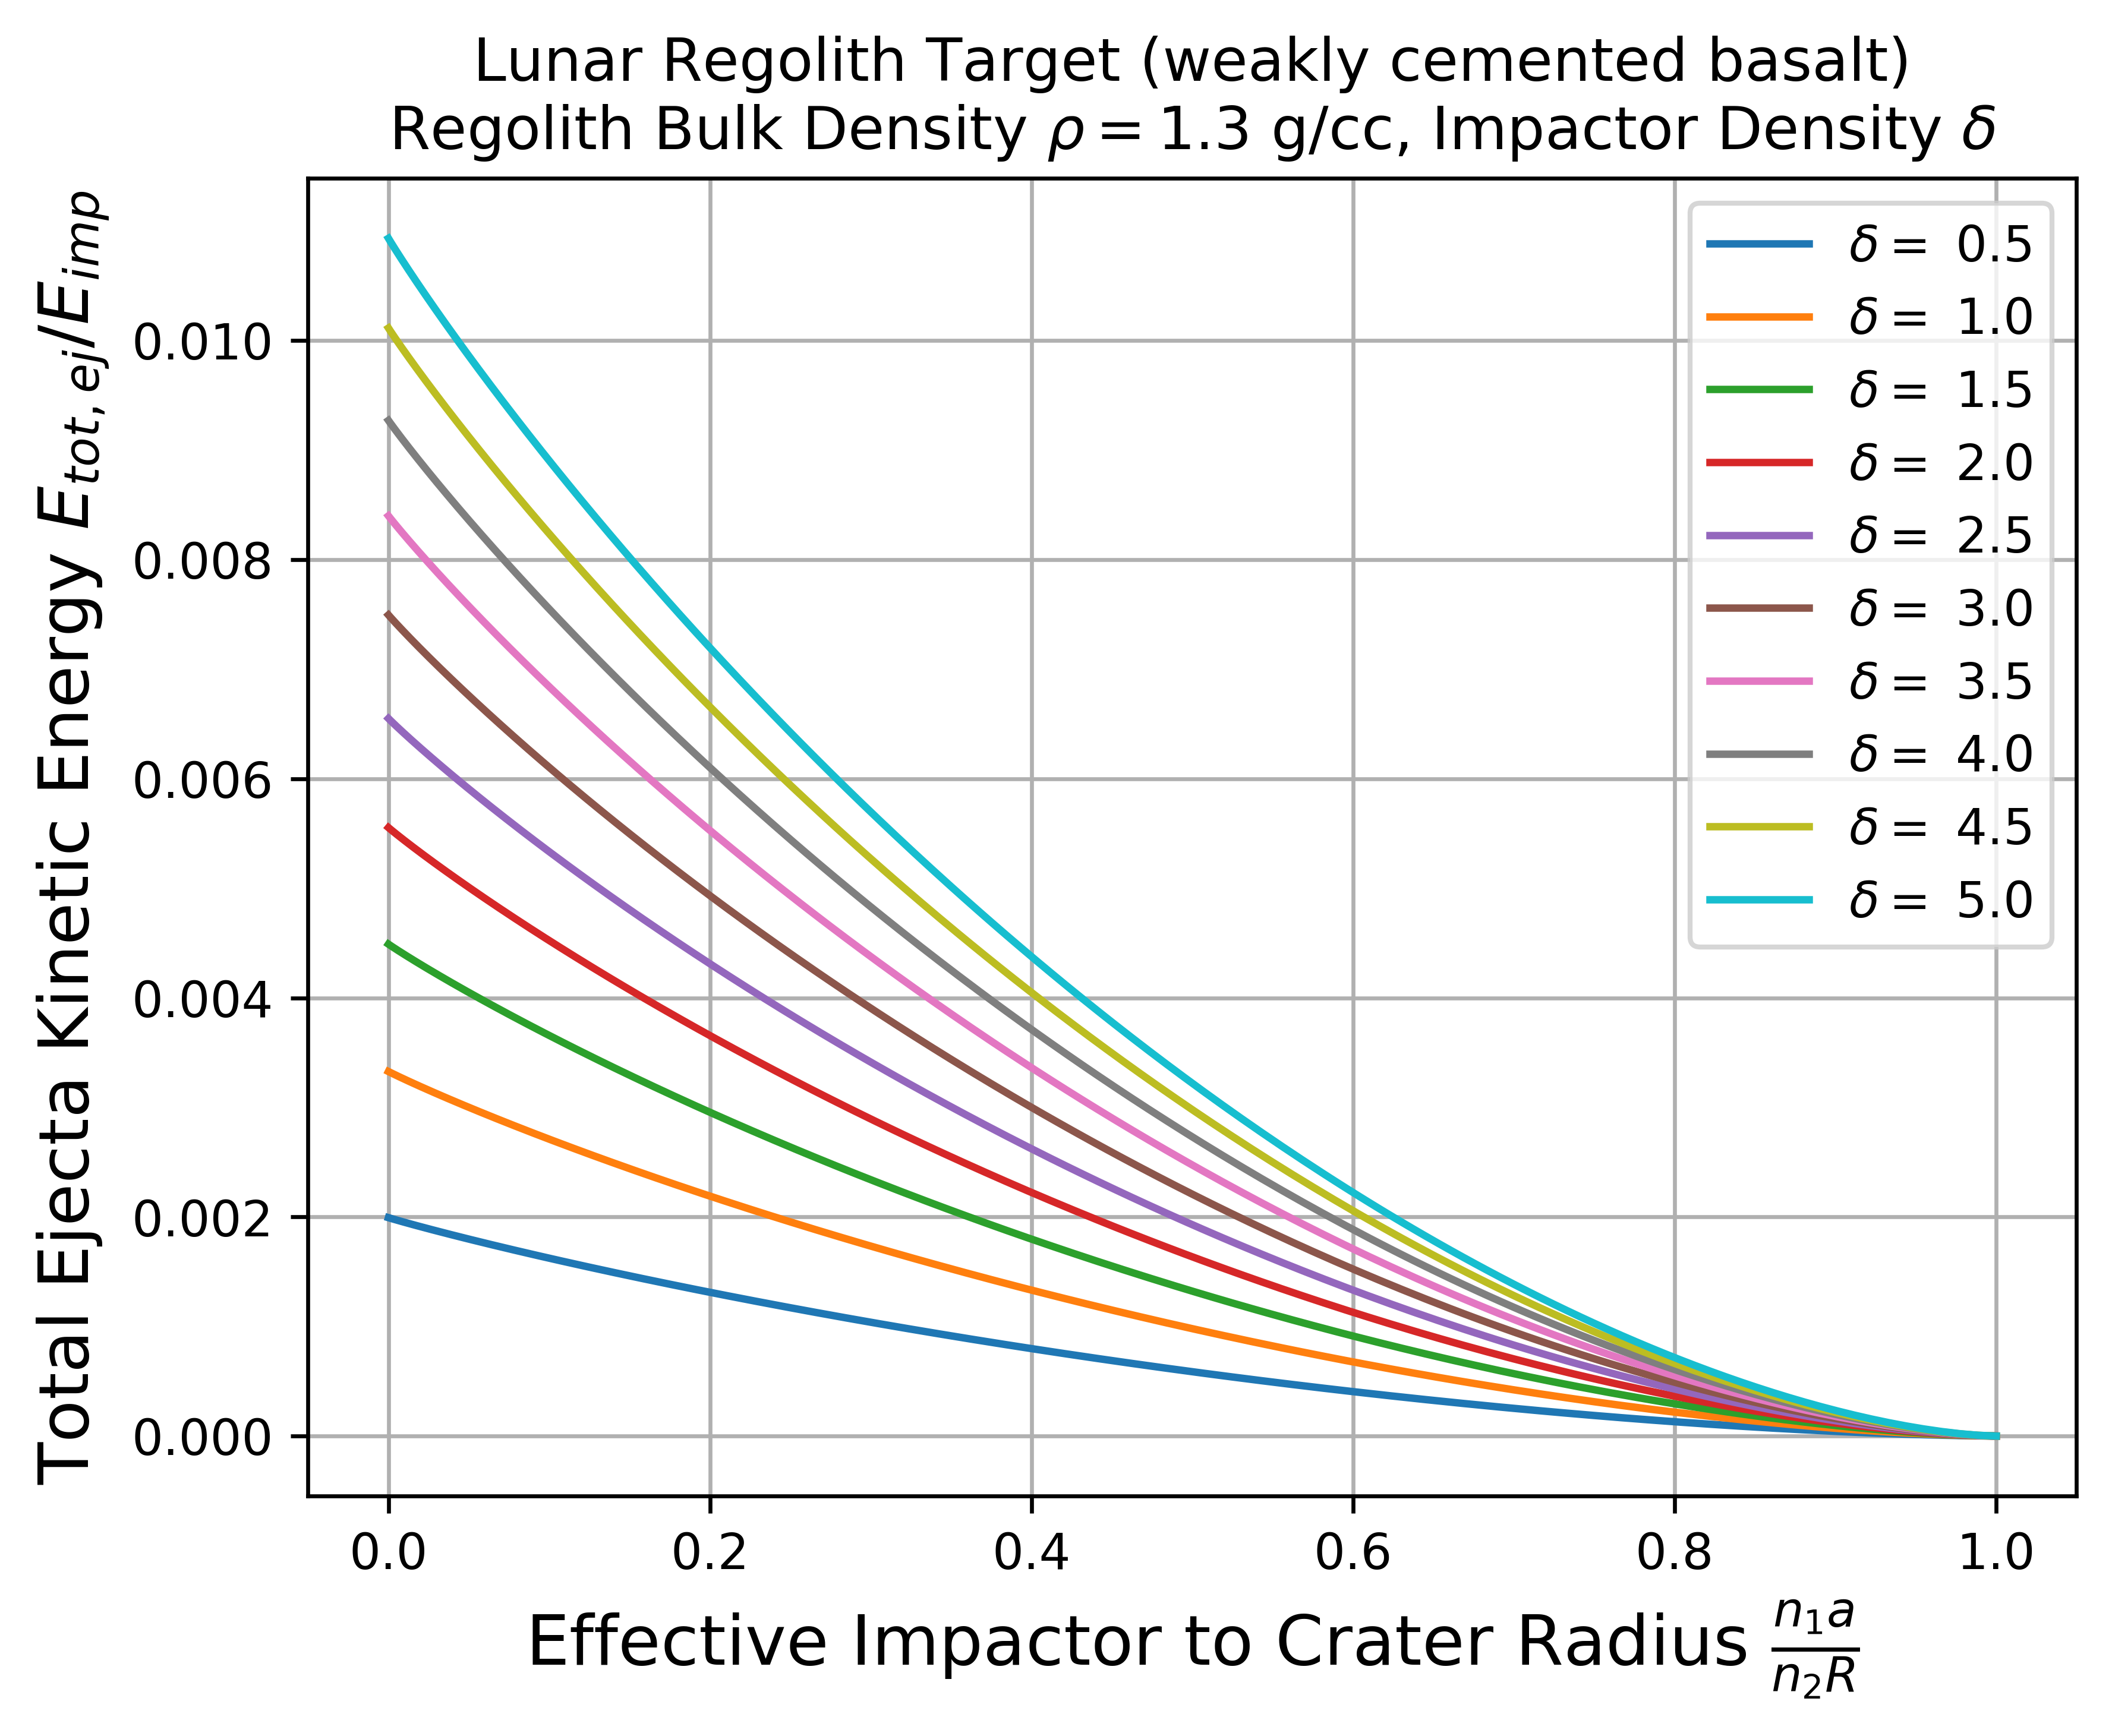
\includegraphics[width=0.65\linewidth]{TotalEjectaKE_vs_EffectiveCraterSize_2.png}
	\caption{The total ejecta kinetic energy $E_{tot,ej}$ (Equation \eqref{eq:Etotej}) over impactor energy $E_{imp} = \frac{1}{2}mU^2$ vs.\ effective impactor to crater radius $\frac{n_1 a}{n_2 R}$ for a lunar regolith target (using WCB in Table~\ref{tab:scaling law parameters}) with regolith surface bulk density $\rho = 1.3$ g/cc and varying impactor densities. }\label{fig:TotalEjectaKE_vs_EffectiveCraterSize_WCB}
\end{figure}

\clearpage

%%%%%%%%%%%%%%%%%%%%%%%%%%%%%%%%%%%%%%%%%%%%%%%%%%%%%%%%%%%%%%%%%%%%%%
\subsection{Orbital Mechanics}\label{ssec:Orbital Mechanics}

Particles that are ejected from the crater are assumed to follow projectile motion in a monopolar gravitational field with no external forces. The equations of motion\footnote{E.g., see \href{http://www.braeunig.us/space/orbmech.htm}{http://www.braeunig.us/space/orbmech.htm}.} the ejecta particles trace are defined by the semi-major axis $a$ and eccentricity $e$ given by
\begin{align}
a &= \frac{1}{\frac{2}{r} - \frac{v^2}{GM}},\label{eq:a_GM}\\
e^2 &= \left(\frac{rv^2}{GM} - 1\right)^2\sin^2\gamma + \cos^2\gamma,\label{eq:e_GM}
\end{align}
for $r$ the orbit position from the gravitating body's center, $v$ the orbit speed, $\gamma$ the local zenith angle with respect to the local horizon, $G = 6.67408\times 10^{-11}$ m$^3$kg$^{-1}$s$^{-2}$ the gravitational constant, and $M = 7.34767\times 10^{22}$ kg the mass of the Moon.

The escape speed of the Moon is defined as
\begin{equation}\label{eq:vesc}
v_{esc} = \sqrt{\frac{2GM}{r_m}},
\end{equation}
where $r_m = 1.7374\times 10^{6}$ m is the radius of the Moon, so that $v_{esc} = 2.376$ km s$^{-1}$. Inserting Equation \eqref{eq:vesc} into Equations \eqref{eq:a_GM} and \eqref{eq:e_GM} gives
\begin{align}
a &= \frac{r_m/2}{\frac{r_m}{r} - \frac{v^2}{v_{esc}^2}},\label{eq:a_vgen}\\
e^2 &= \left(\frac{2rv^2}{r_m v_{esc}^2} - 1\right)^2\sin^2\gamma + \cos^2\gamma.\label{eq:e_vgen}
\end{align}

If the definitions of $a$ and $e$ are at a point on the surface of the Moon, $r = r_m$, then Equations \eqref{eq:a_vgen} and \eqref{eq:e_vgen} become
\begin{align}
a &= \frac{r_m/2}{1 - \frac{v_p^2}{v_{esc}^2}},\label{eq:a_vrm}\\
e^2 &= \left(\frac{2v_p^2}{v_{esc}^2} - 1\right)^2\sin^2\gamma_p + \cos^2\gamma_p.\label{eq:e_vrm}
\end{align}

The position $r$ of the ejected particle in its orbit is given by
\begin{equation}\label{eq:r_orbit}
r = \frac{a(1-e^2)}{1+e\cos\beta},
\end{equation}
where $\beta$ is the true anomaly or angle from the periapsis point. An angle of $\beta=0$ would be a particle at the periapsis and an angle of $\beta=\pi$ would be a particle at the apoapsis point.

In terms of the true anomaly $\beta$, the local zenith angle of the particle is given by
\begin{equation}\label{eq:tan_gamma}
\tan\gamma = \frac{1+e\cos\beta}{e\sin\beta}.
\end{equation}

In the following two sections, the initial/final speeds $v_p$ and $v_s$, the final zenith angle $\gamma_s$, and the final position in the orbit at the asset $r_s$ will be computed. Section \ref{sssec:Crater on Surface to Observer at Surface} will be a special case where the final impact point at the asset is at the surface of the Moon and Section \ref{sssec:Crater on Surface to Observer at or above Surface} will assume a more general case of an arbitrary position on or above the Moon for the asset.

%%%%%%%%%%%%%%%%%%%%%%%%%%%%%%%%%%%%%%%%%%%%%%%%%%%%%%%%%%%%%%%%%%%%%%
\subsubsection{Crater on Surface to Asset at Surface}\label{sssec:Crater on Surface to Observer at Surface}
% include final speed and zenith
The position in the orbit from the crater is the same radius is that of the asset at the surface, which says that the angle of periapsis at the crater impact is $\beta_p$ and at the asset is $\beta_s=-\beta_p$. Therefore, the selenographic distance between the two points is
\begin{align}
\frac{D}{r_m} &= \beta_s - \beta_p,\\
&= 2(\pi - \beta_p),
\end{align}
and solving for $\beta_p$,
\begin{equation}\label{eq:betap_specialcase}
\beta_p = \pi - \frac{D}{2r_m}.
\end{equation}

\subsubsubsection{Distance $D$ vs.\ $v_p$ and $\gamma_p$}
Solving Equation \eqref{eq:r_orbit} for $\cos\beta_p$ and also $\sin\beta_p$, making use of $a$ and $e$ defined at the crater point (Equations \eqref{eq:a_vrm} and \eqref{eq:e_vrm}):
\begin{align}\label{eq:ecosbetap}
e\cos\beta_p &= 2\frac{v_p^2}{v_{esc}^2}\sin^2\gamma_p - 1,\\
e\sin\beta_p &= 2\frac{v_p^2}{v_{esc}^2}\sin\gamma_p\cos\gamma_p.\label{eq:esinbetap}
\end{align}
Therefore, taking the tangent\footnote{Note, $\tan(\pi-\eta) = -\tan\eta$.} and plugging in Equation \eqref{eq:betap_specialcase}, (c.f., Equation (1) of \cite{vickery1986size})
\begin{equation}\label{eq:D_special_case}
\tan\left(\frac{D}{2r_m}\right) = \frac{2\frac{v_p^2}{v_{esc}^2}\sin\gamma_p\cos\gamma_p}{1 - 2\frac{v_p^2}{v_{esc}^2}\sin^2\gamma_p}.
\end{equation}
The distance at which the ejecta reaches apoapsis can be found by substituting $D = 2D_{ap}$ into Equation \eqref{eq:D_special_case}.

\subsubsubsection{Initial Speed $v_p$ vs.\ $D$ and $\gamma_p$}
The initial speed $v_p$ can be solved for, giving
\begin{equation}\label{eq:vp_special_case}
\frac{v_p}{v_{esc}} = \frac{1}{\sqrt{1-\cos(2\gamma_p) + \sin(2\gamma_p)\cot\left(\frac{D}{2r_m}\right)}}.
\end{equation}

\subsubsubsection{Initial Zenith Angle $\gamma_p$ vs.\ $D$ and $v_p$}
The initial zenith angle $\gamma_p$ can also be solved for by expanding $\cos(2\gamma_p)$ and $\sin(2\gamma_p)$ in terms of $\cot\gamma_p$,
\begin{align}\label{eq:1-cos 2g to cot g}
1-\cos(2\gamma_p) &= \frac{2}{1+\cot^2\gamma_p},\\\label{eq:sin 2g to cot g}
\sin(2\gamma_p) &= \frac{2\cot\gamma_p}{1+\cot^2\gamma_p},
\end{align}
such that
\begin{equation}\label{eq:specialcase gammap}
\cot\gamma_p = \frac{v_p^2}{v_{esc}^2}\cot\left(\frac{D}{2r_m}\right) \pm \sqrt{\frac{v_p^4}{v_{esc}^4}\cot^2\left(\frac{D}{2r_m}\right) + 2\frac{v_p^2}{v_{esc}^2}-1}.
\end{equation}
The plus case gives $\gamma_p \le \gamma_{p,opt}$ and the minus case gives  $\gamma_p \ge \gamma_{p,opt}$.

\subsubsubsection{Minimum Initial Zenith Angle $\gamma_{p,min}$ vs.\ $D$}
To find the minimum initial zenith angle $\gamma_{p,min}$, the initial speed approaches the escape speed $v_p\to v_{esc}$ in Equation \eqref{eq:specialcase gammap} and simplifying (taking the positive case),
\begin{equation}\label{eq:gpmin_special}
\gamma_{p,min} = \frac{D}{4r_m}.
\end{equation}


\subsubsubsection{Maximum Distance $D_{max}$ vs.\ $v_p$}
The maximum distance $D_{max}$ a particle can travel at a given speed and optimal zenith angle is found by taking the discriminant in Equation \eqref{eq:specialcase gammap} and setting it equal to zero such that
\begin{equation}\label{eq:Dmax}
\tan\left(\frac{D_{max}}{2r_m}\right) = \pm\frac{v_p^2/v_{esc}^2}{\sqrt{1-2v_p^2/v_{esc}^2}}
\end{equation}
where the direct path is the positive case, and the indirect path is the negative case with modding the tangent argument by $\pi$.
%\begin{equation}\label{eq:Dmax}
%\frac{D_{max}}{2r_m} =
%\begin{cases}
%\arctan\left(\frac{v_p^2/v_{esc}^2}{\sqrt{1-2v_p^2/v_{esc}^2}}\right) \text{, direct path ($D \le \pi r_m$)}\\
%\pi - \arctan\left(\frac{v_p^2/v_{esc}^2}{\sqrt{1-2v_p^2/v_{esc}^2}}\right) \text{, indirect path ($D \ge \pi r_m$)}
%\end{cases}, 
%\end{equation}

\subsubsubsection{Minimum Initial Speed $v_{p,min}$ vs.\ $D$}
The minimum speed $v_{p,min}$ at which to travel a certain distance is found by solving for $v_p$ in Equation \eqref{eq:Dmax}, giving
\begin{equation}\label{eq:vpmin_special}
\frac{v_{p,min}^2}{v_{esc}^2} = +\tan\left(\frac{D}{2r_m}\right)\tan\left(\frac{\pi}{4}- \frac{D}{4r_m}\right),
\end{equation}
for $D \le \pi r_m$. For further distances, the limiting minimum speed is $v_{p,min}/v_{esc} = \sqrt{2}/2$.

\subsubsubsection{Optimal Initial Zenith Angle $\gamma_{p,opt}$ vs.\ $D$}
The optimal initial zenith angle $\gamma_{p,opt}$ follows as\footnote{Note that $\arctan(\cot(\theta)) = \pi/2 - \theta$ for $0 \le \theta \le \pi$.}
\begin{equation}
\gamma_{p,opt} = \frac{\pi}{4} + \frac{D}{4r_m},
\end{equation}
for $D \le \pi r_m$. For further distances, the limiting optimal angle is $\gamma_{p,opt} = \pi/2$. At very small distances $D \ll r_m$, the optimal angle is $\sim 45^\circ$ as expected.

\subsubsubsection{Final Speed $v_s$ and Zenith Angle $\gamma_s$}
Due to the symmetry of the orbit points, the final speed and zenith angle\footnote{The final zenith angle is taken as the observed incoming angle, not the angle at which the ejecta is going. This introduces a different of $\pi$ radians.} are given by
\begin{align}
v_s &= v_p,\\
\gamma_s &= \gamma_p.
\end{align}

\clearpage
\subsubsubsection{Visualizing Ejecta in Phase Space}

\begin{figure}[!htb]
	\centering
	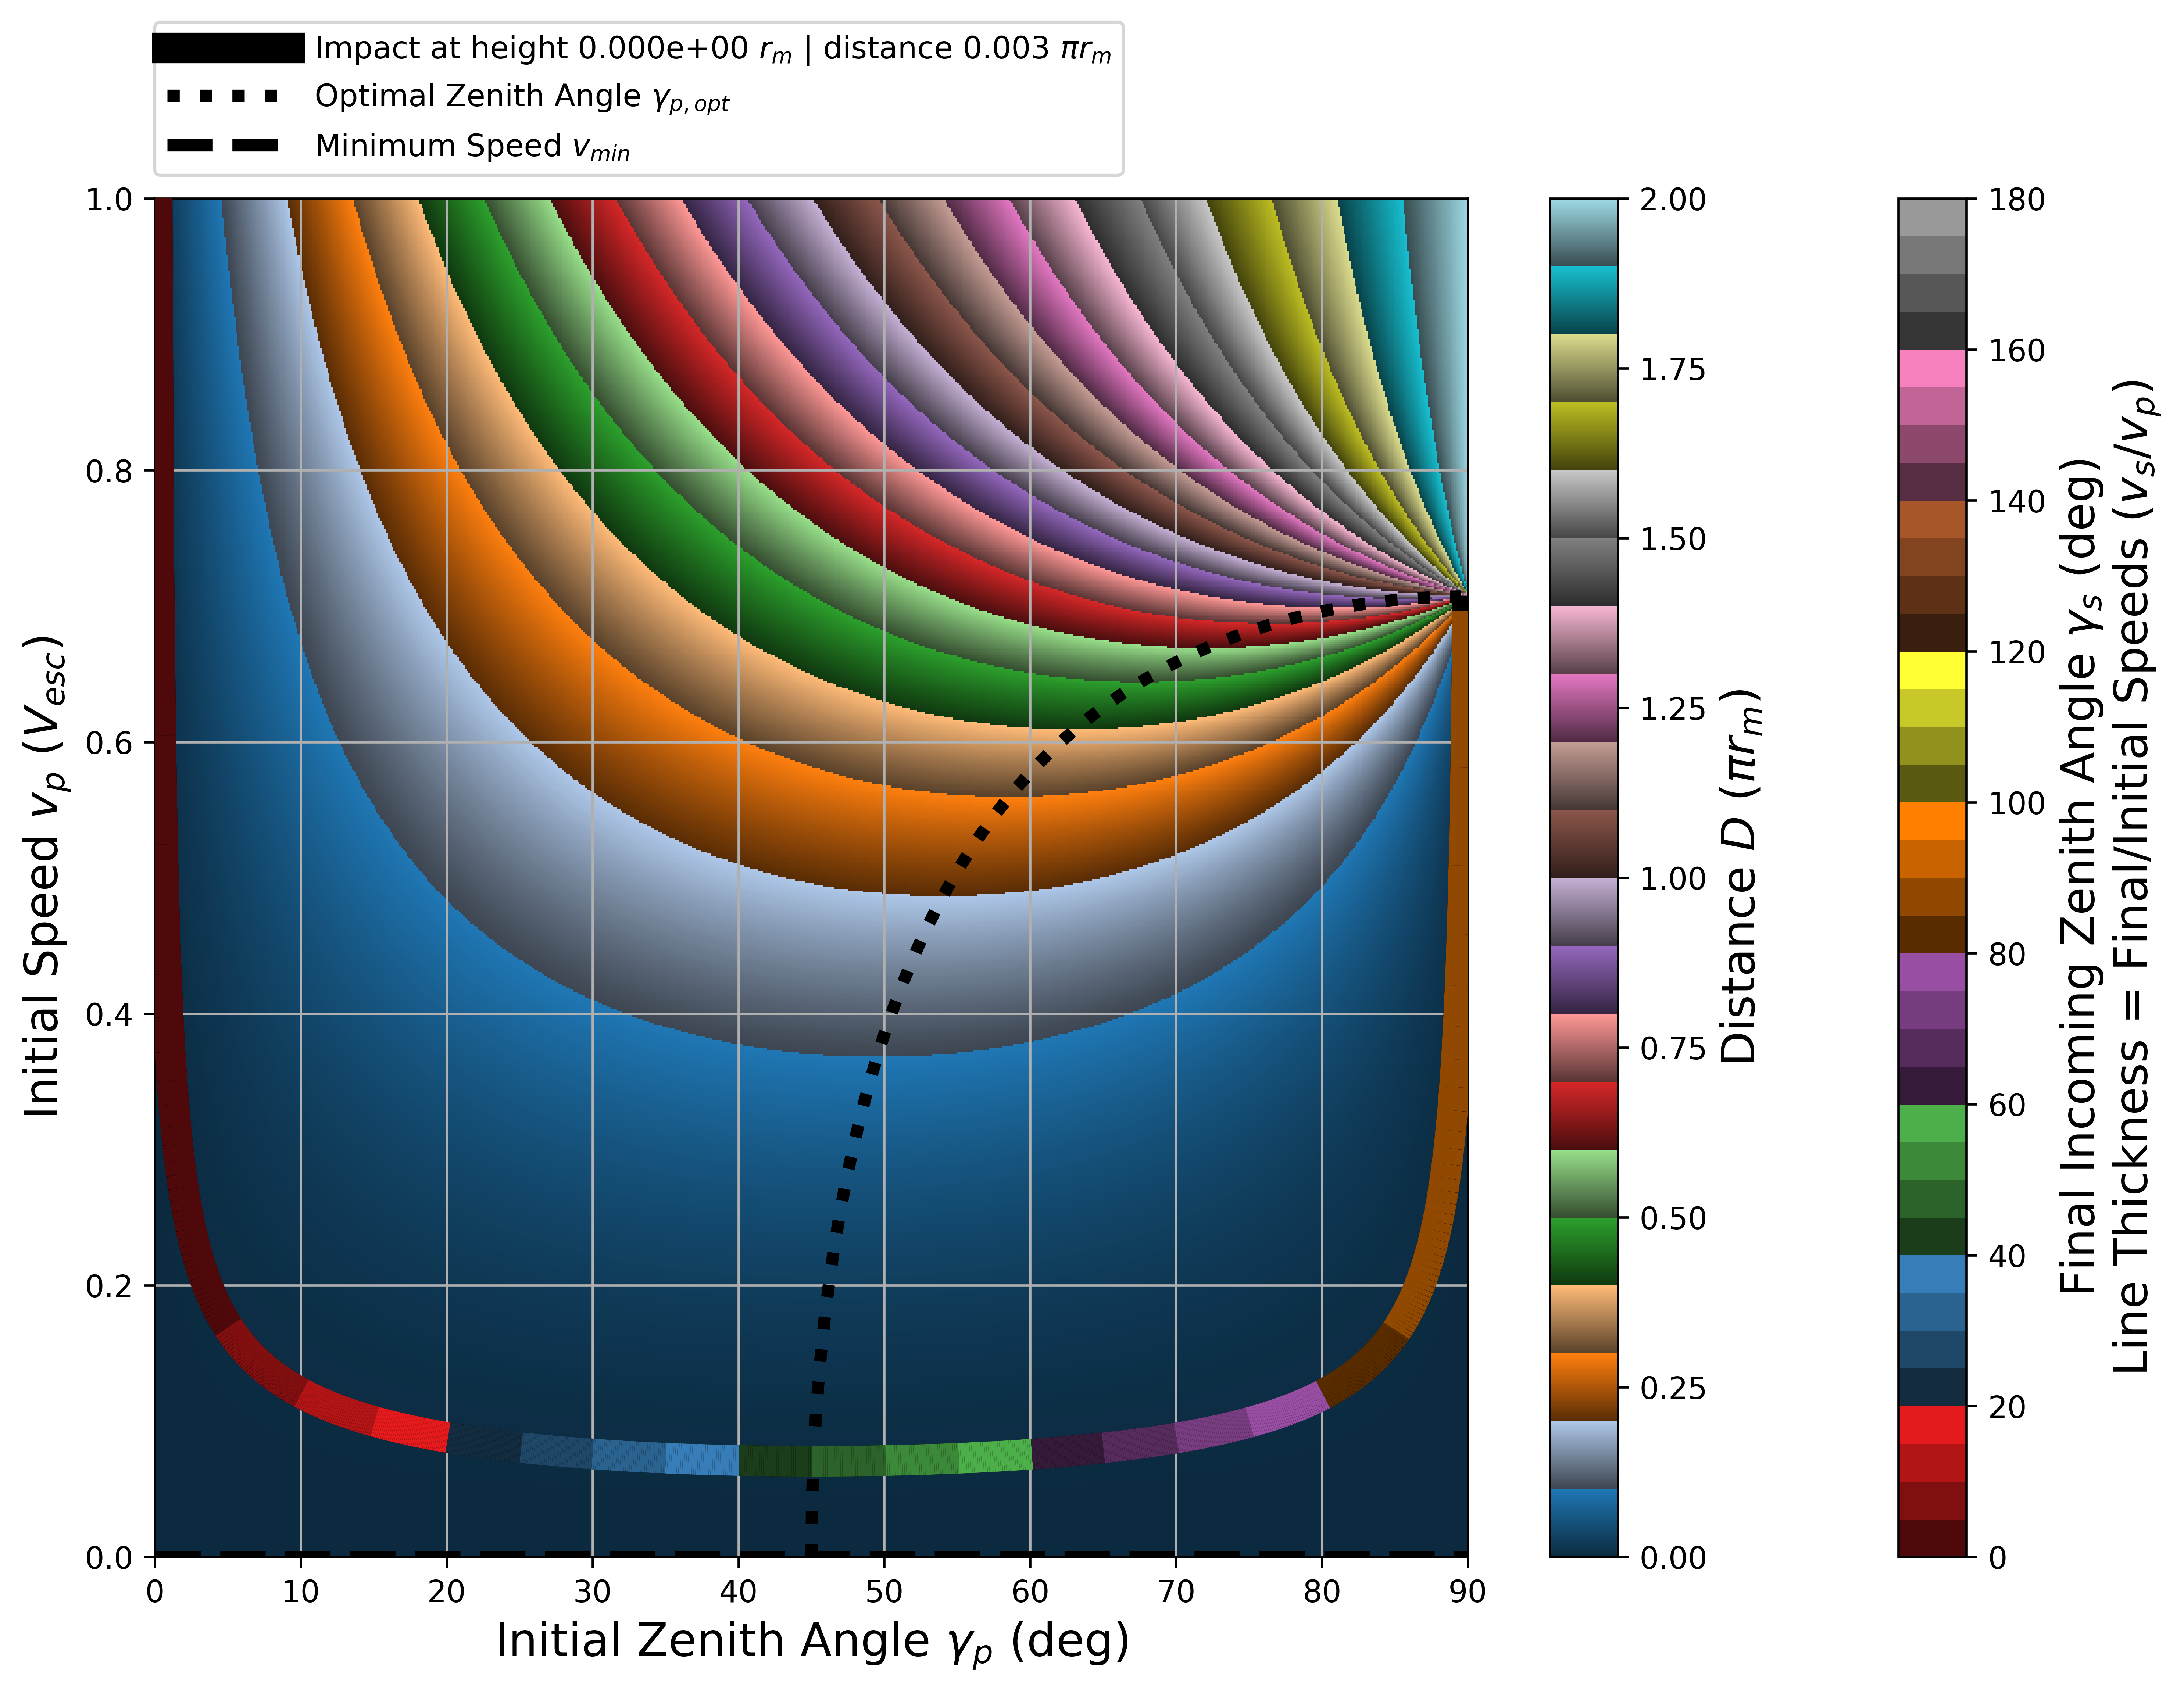
\includegraphics[width=1.00\linewidth]{dist_speed_zenith_plot_000_0.000e+00_0.010.png}
	\caption{The initial speed $v_p$ vs.\ initial zenith angle $\gamma_p$ as a function of distance $D$ is shown with a distance contour line at $0.003\pi r_m$ with a point-asset altitude of $0 r_m$ (on the lunar surface). The contour line's color depicts the final incomming zenith angle $\gamma_s$ where the thickness of the line gives the ratio of the final and initial speeds $v_s/v_p$. For a point-asset at the surface, this ratio will always be $1$. The intersection of the distance contour line and the black dotted line gives the optimal zenith angle $\gamma_{p,opt}$ (Equation~\eqref{eq:gamma p ap 1}), i.e.\ the slowest initial speed to reach the contour line distance of $0.003\pi r_m$. Since the point-asset is on the lunar surface, there is no minimum bound on the speed (denoted by the black dashed line).
	}\label{fig:dist_speed_zenith_plot_000_0.000e+00_0.010}
\end{figure}

\begin{figure}[!htb]
	\centering
	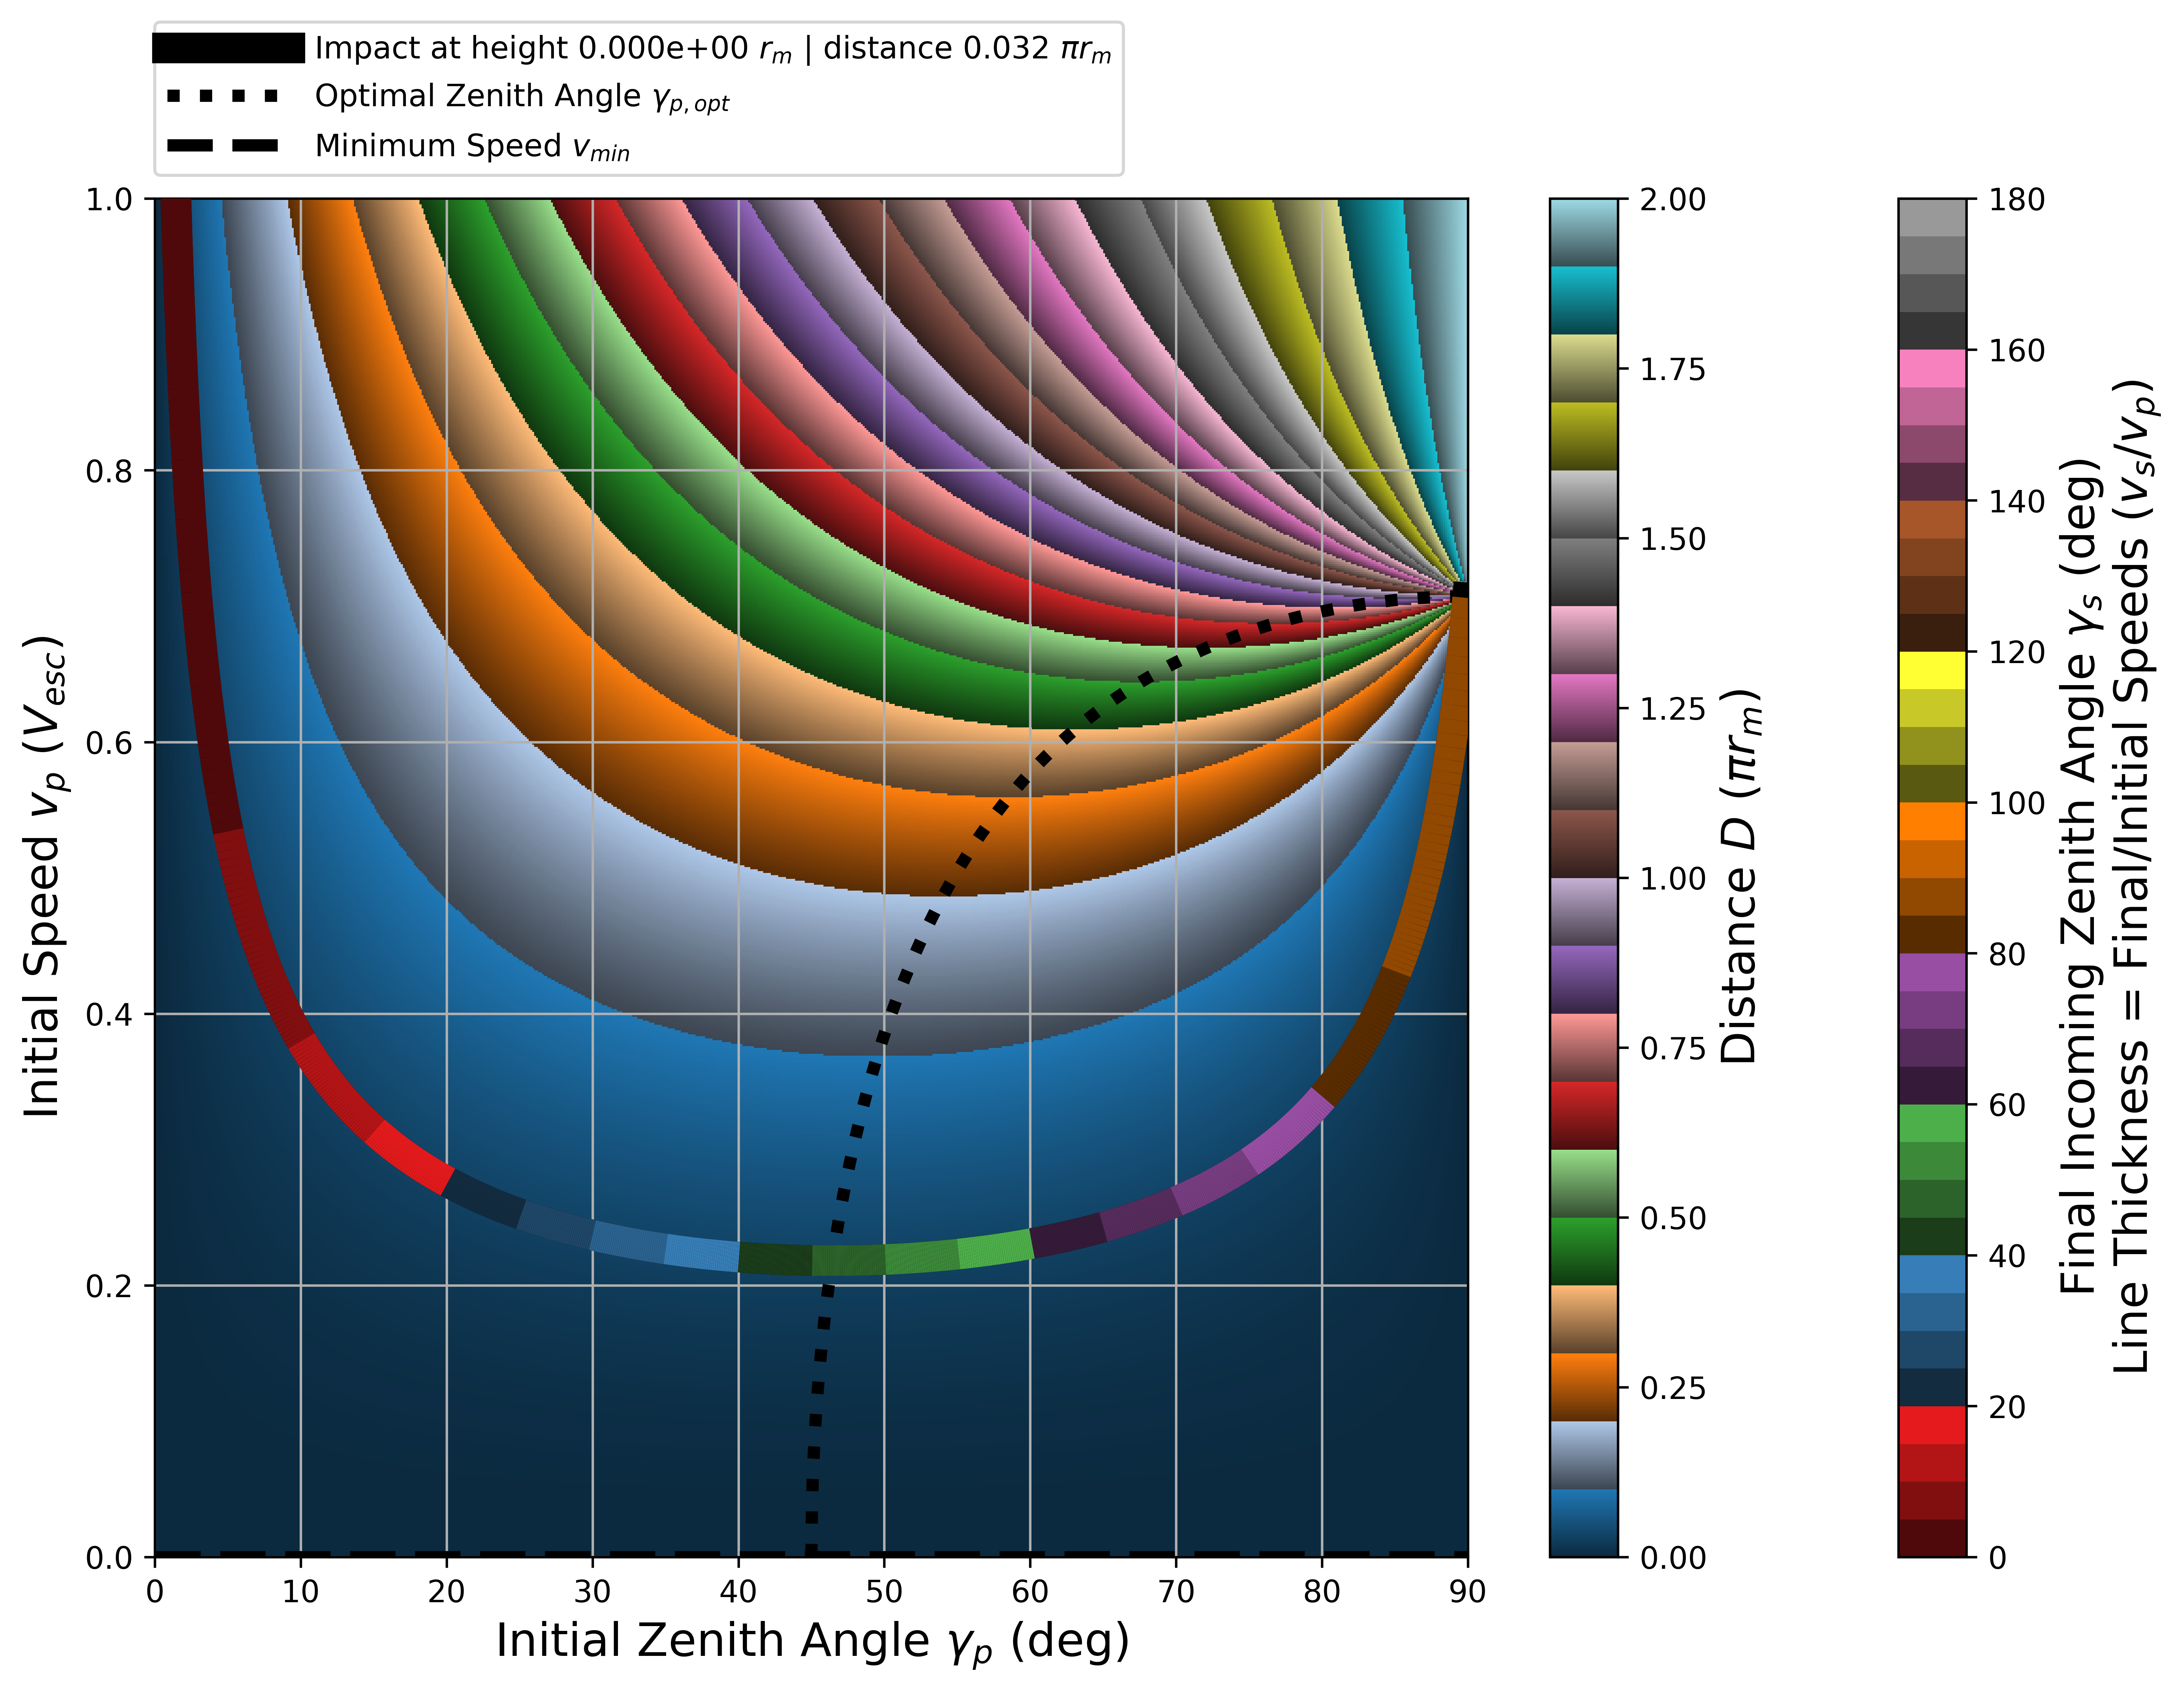
\includegraphics[width=1.00\linewidth]{dist_speed_zenith_plot_001_0.000e+00_0.100.png}
	\caption{The initial speed $v_p$ vs.\ initial zenith angle $\gamma_p$ as a function of distance $D$ is shown with a distance contour line at $0.032\pi r_m$ with a point-asset altitude of $0 r_m$ (on the lunar surface). The contour line's color depicts the final incomming zenith angle $\gamma_s$ where the thickness of the line gives the ratio of the final and initial speeds $v_s/v_p$. For a point-asset at the surface, this ratio will always be $1$. The intersection of the distance contour line and the black dotted line gives the optimal zenith angle $\gamma_{p,opt}$ (Equation~\eqref{eq:gamma p ap 1}), i.e.\ the slowest initial speed to reach the contour line distance of $0.032\pi r_m$. Since the point-asset is on the lunar surface, there is no minimum bound on the speed (denoted by the black dashed line).}\label{fig:dist_speed_zenith_plot_001_0.000e+00_0.100}
\end{figure}

\begin{figure}[!htb]
	\centering
	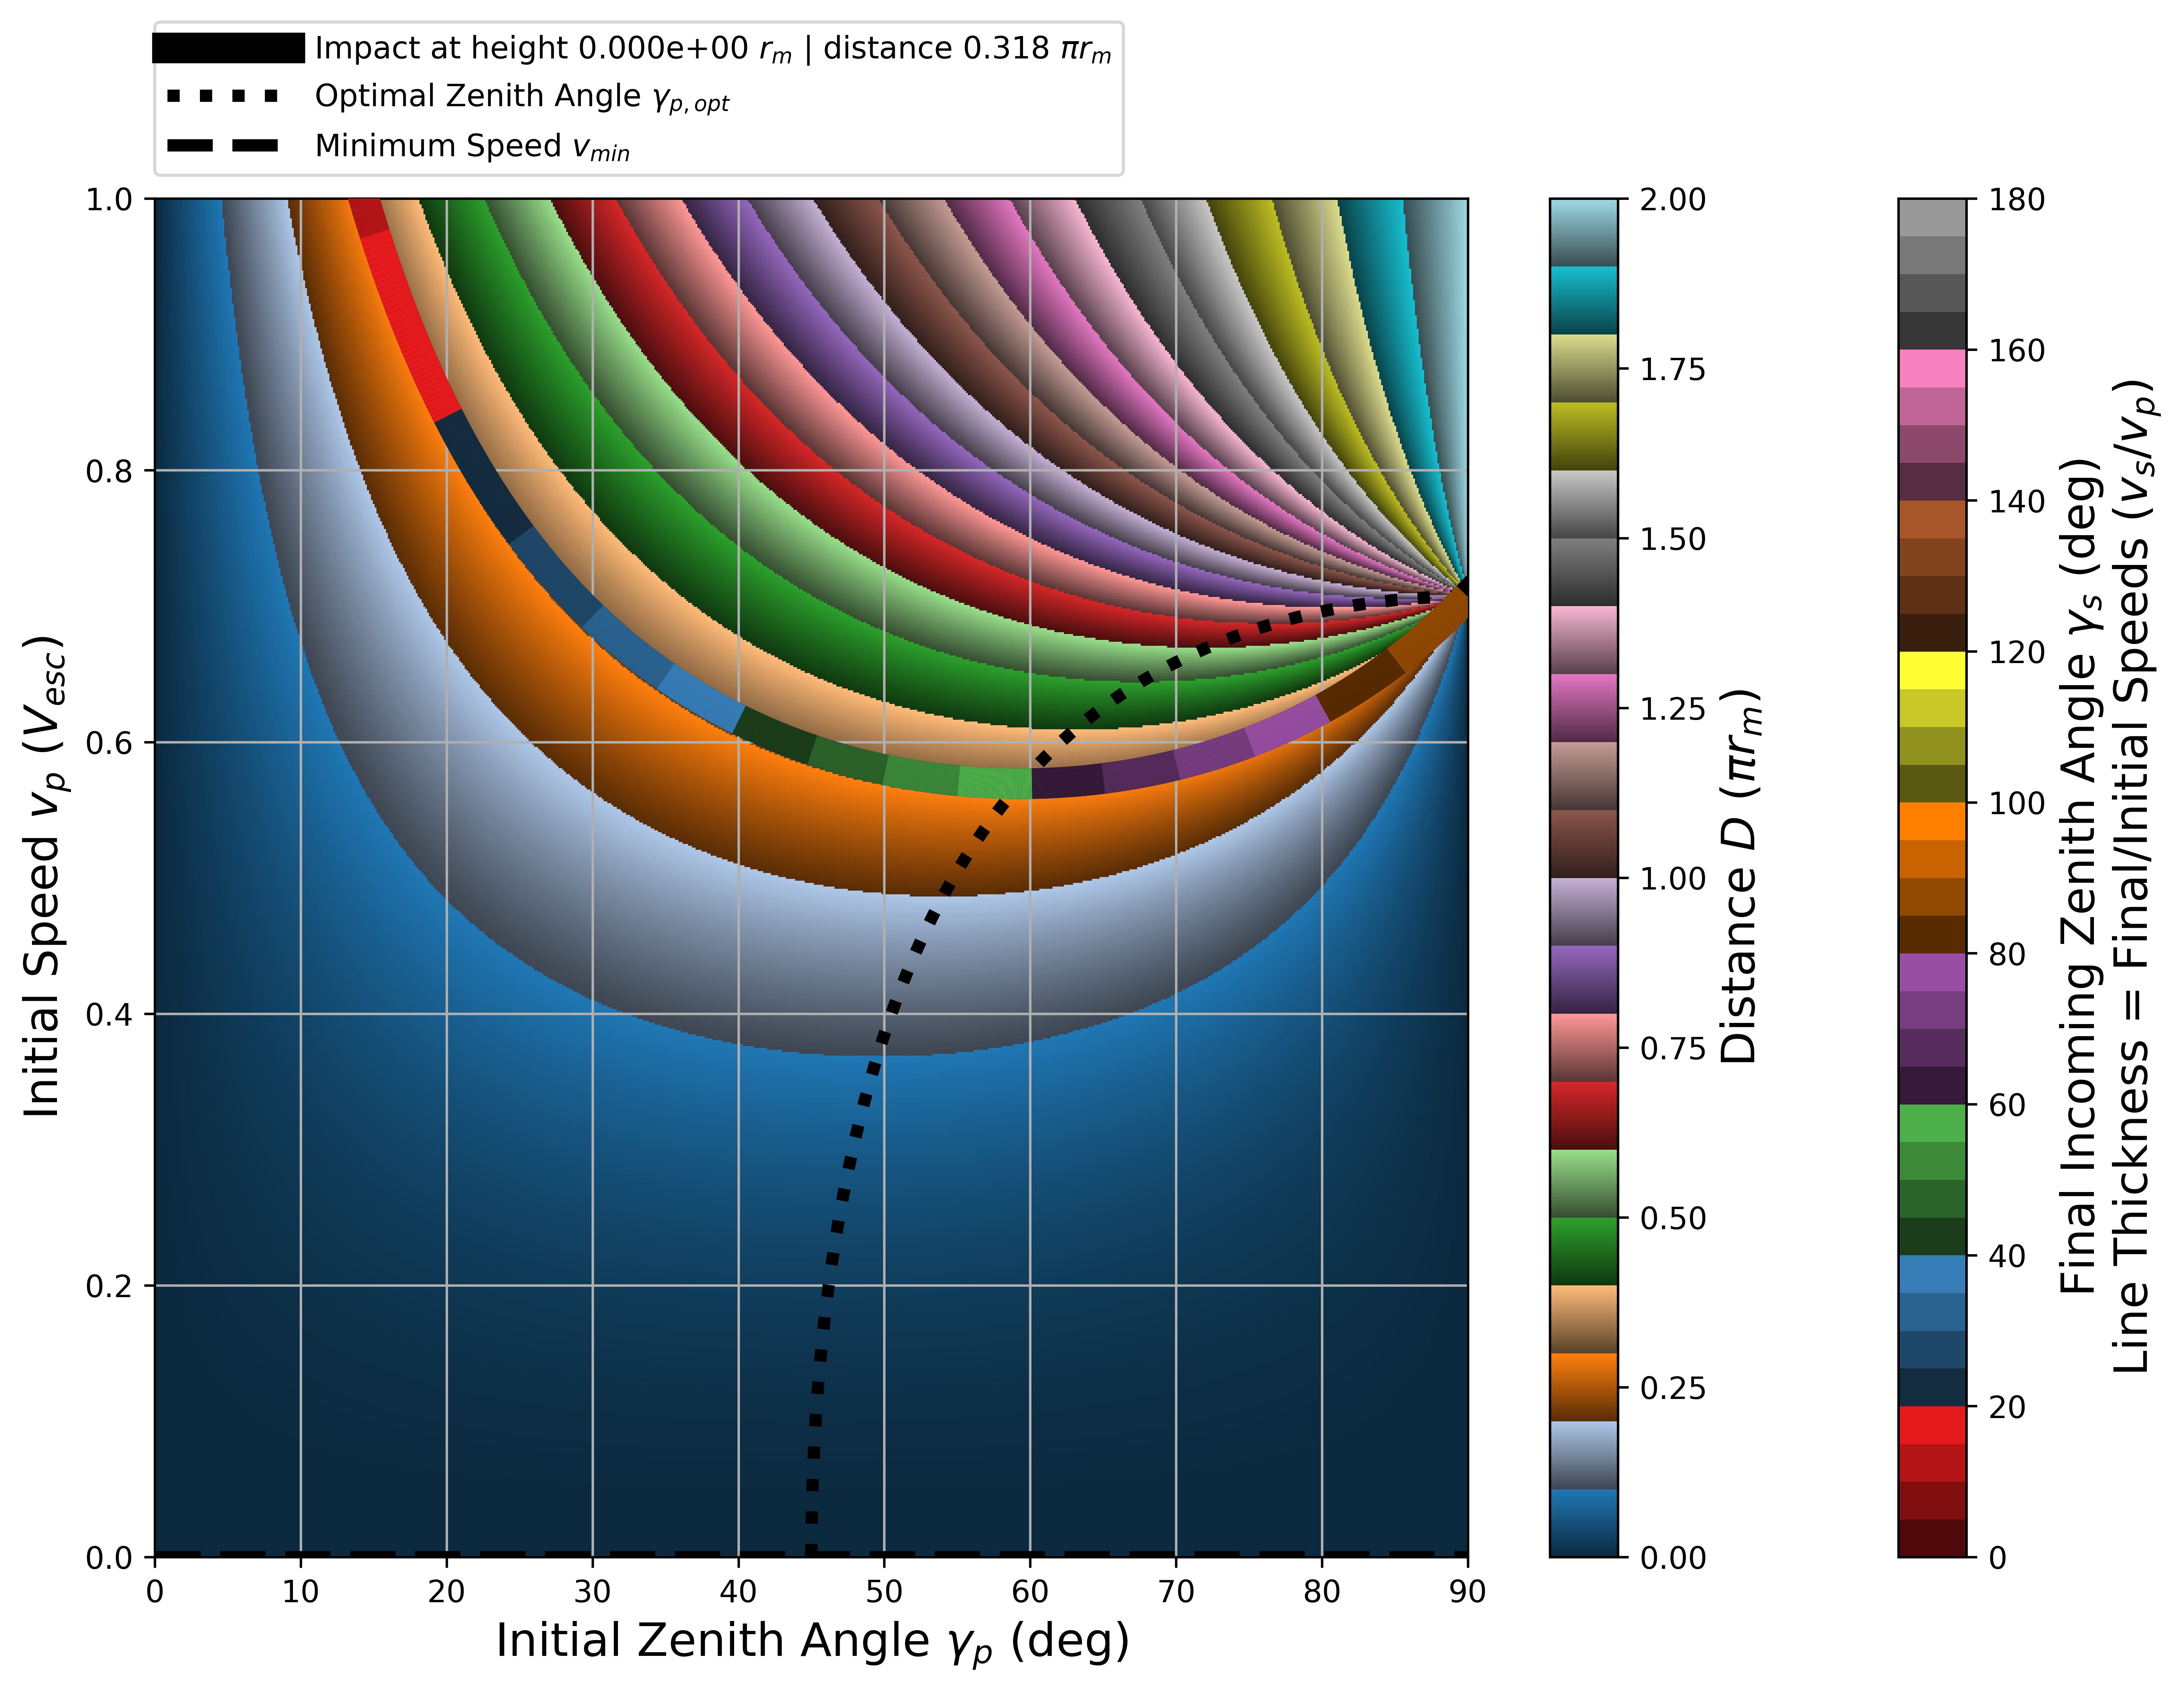
\includegraphics[width=1.00\linewidth]{dist_speed_zenith_plot_002_0.000e+00_1.000.png}
	\caption{The initial speed $v_p$ vs.\ initial zenith angle $\gamma_p$ as a function of distance $D$ is shown with a distance contour line at $0.318\pi r_m$ with a point-asset altitude of $0 r_m$ (on the lunar surface). The contour line's color depicts the final incomming zenith angle $\gamma_s$ where the thickness of the line gives the ratio of the final and initial speeds $v_s/v_p$. For a point-asset at the surface, this ratio will always be $1$. The intersection of the distance contour line and the black dotted line gives the optimal zenith angle $\gamma_{p,opt}$ (Equation~\eqref{eq:gamma p ap 1}), i.e.\ the slowest initial speed to reach the contour line distance of $0.318\pi r_m$. Since the point-asset is on the lunar surface, there is no minimum bound on the speed (denoted by the black dashed line).}\label{fig:dist_speed_zenith_plot_002_0.000e+00_1.000}
\end{figure}

\begin{figure}[!htb]
	\centering
	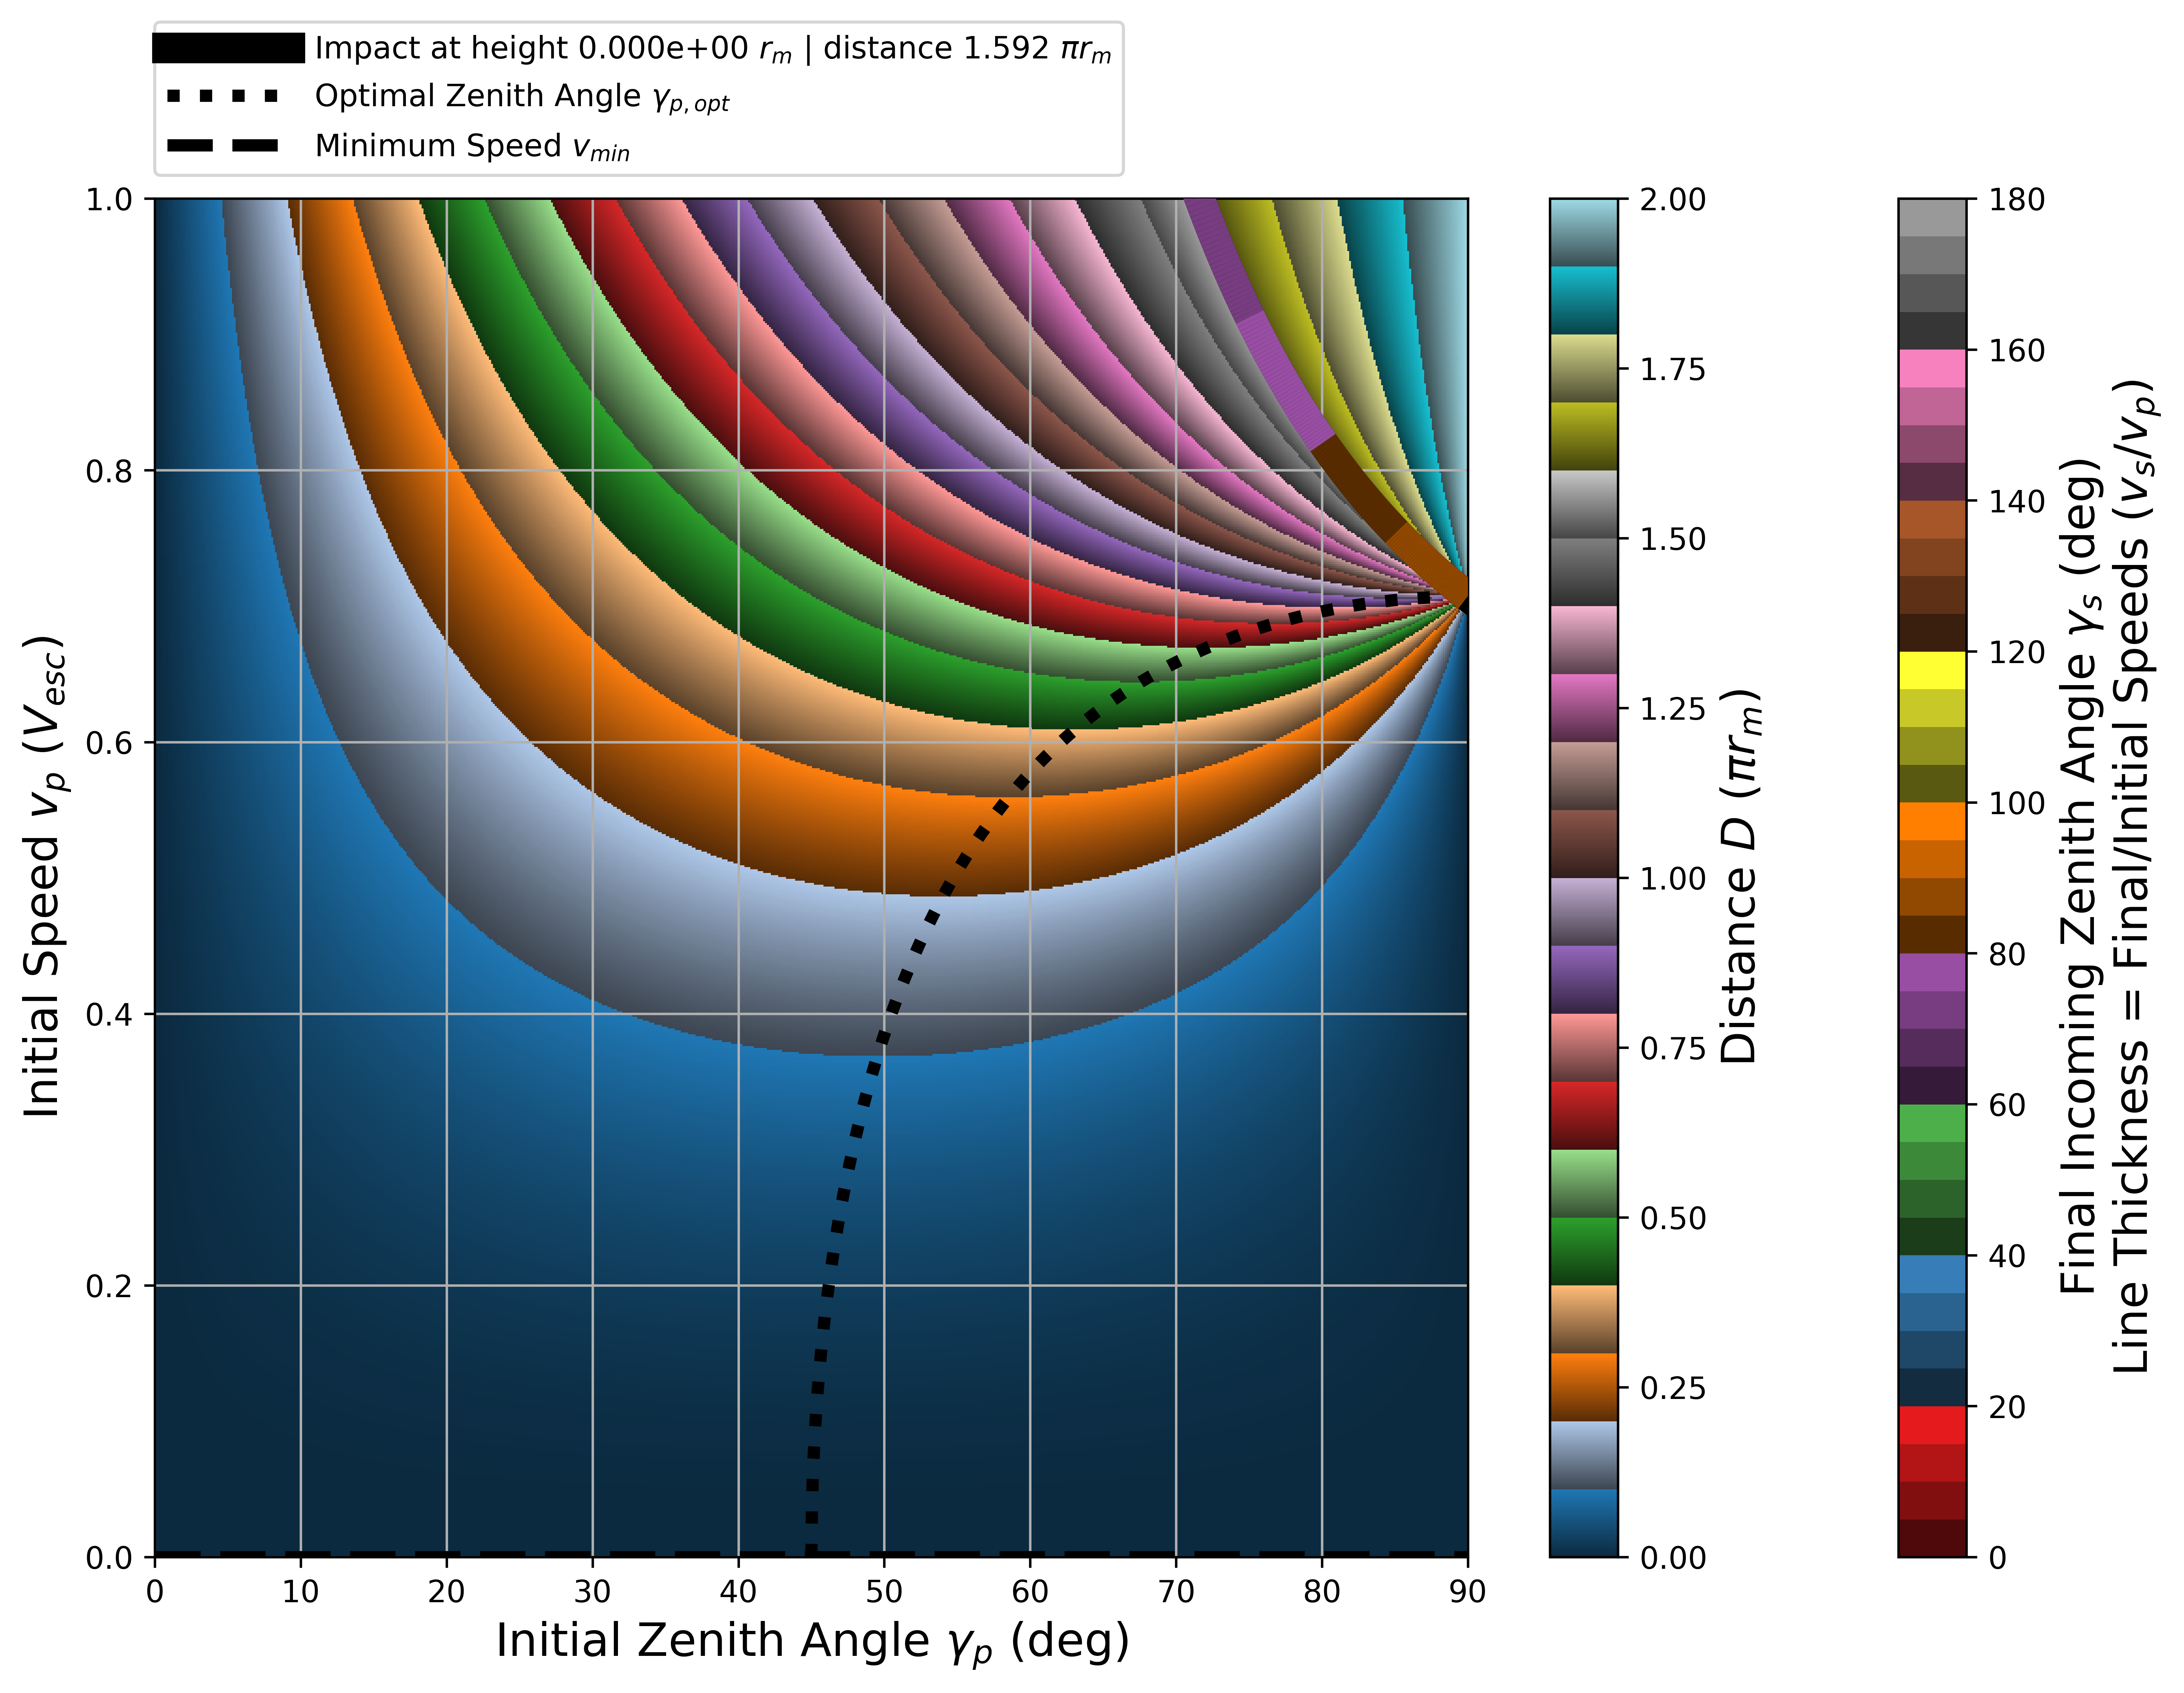
\includegraphics[width=1.00\linewidth]{dist_speed_zenith_plot_003_0.000e+00_5.000.png}
	\caption{The initial speed $v_p$ vs.\ initial zenith angle $\gamma_p$ as a function of distance $D$ is shown with a distance contour line at $1.592\pi r_m$ (past the antipode) with a point-asset altitude of $0 r_m$ (on the lunar surface). The contour line's color depicts the final incomming zenith angle $\gamma_s$ where the thickness of the line gives the ratio of the final and initial speeds $v_s/v_p$. For a point-asset at the surface, this ratio will always be $1$. The intersection of the distance contour line and the black dotted line gives the optimal zenith angle $\gamma_{p,opt}$ (Equation~
		\eqref{eq:gamma p ap 1}), i.e.\ the slowest initial speed to reach the contour line distance of $1.592\pi r_m$. Since the point-asset is on the lunar surface, there is no minimum bound on the speed (denoted by the black dashed line).}\label{fig:dist_speed_zenith_plot_003_0.000e+00_5.000}
\end{figure}

\clearpage



%%%%%%%%%%%%%%%%%%%%%%%%%%%%%%%%%%%%%%%%%%%%%%%%%%%%%%%%%%%%%%%%%%%%%%
\subsubsection{Crater on Surface to Asset at or above Surface}\label{sssec:Crater on Surface to Observer at or above Surface}
% include final speed and zenith

In general, it is assumed that the final position at the asset can be either at the surface or above the surface of the Moon. The selenographic distance between the initial and final points are the same as before, given as
\begin{equation}\label{eq:D_beta_gen}
\frac{D}{r_m} = \beta_s - \beta_p,
\end{equation}
however, $\beta_s$ is kept ambiguous.

First, equations for $e\cos\beta_s$ and $e\sin\beta_s$ are solved for using Equations \eqref{eq:r_orbit} and \eqref{eq:e_vrm}, giving
\begin{align}\label{eq:ecosbetas}
e\cos\beta_s &= 2\frac{r_m}{r_s}\frac{v_p^2}{v_{esc}^2}\sin^2\gamma_p - 1,\\
e\sin\beta_s &= 2\frac{r_m}{r_s}\frac{v_p^2}{v_{esc}^2}\sin\gamma_p\cos\gamma_p F(v_p,\gamma_p,r_s), \label{eq:esinbetas}
\end{align}
where
\begin{equation}\label{eq:F}
F(v_p,\gamma_p,r_s) = \pm\sqrt{1 + \frac{\frac{r_s}{r_m}-1}{\cos^2\gamma_p}\left(\frac{r_s}{r_m}+1-\frac{r_s/r_m}{v_p^2/v_{esc}^2}\right)}.
\end{equation}
The sign of $F$ is summarized by
\begin{equation}\label{eq:sign of F} %and $D < \pi r_m$
sign(F) = \begin{cases}
+ \text{, $\gamma_p > \gamma_{p,ap}$ (incoming below local horizon)}\\
- \text{, otherwise (incoming above local horizon)}
\end{cases}.
\end{equation}
Plugging in the initial speed $v_p$ (Equation \eqref{eq:vp_gen_case}) into Equation \eqref{eq:F}, the sign of $F$ becomes implicit in the equation and reads:
\begin{equation}
F(D,\gamma_p,r_s) = \left(\frac{r_s}{r_m}-1\right)\frac{\tan\gamma_p}{\tan\left(\frac{D}{2r_m}\right)} - \frac{r_s}{r_m}.
\end{equation}

\subsubsubsection{Maximum Radial Distance $r_{max}$ vs.\ $v_p$ and $\gamma_p$}
Note that the maximum radius by definition occurs at the apoapsis, or $\beta_s=\pi$, such that Equation \eqref{eq:r_orbit} becomes (fixing the typo in Equation 16 of \cite{gault1963spray})
\begin{equation}\label{eq:rmax}
\frac{r_{max}}{r_m} = \frac{1 + \sqrt{\left(\frac{2v_p^2}{v_{esc}^2}-1\right)^2\sin^2\gamma_p+\cos^2\gamma_p}}{2\left(1-\frac{v_p^2}{v_{esc}^2}\right)},
\end{equation}
which is also the solution to $F(v_p,\gamma_p,r_s) = 0$ and solving for $r_s$, i.e.\ $F(v_p,\gamma_p,r_{max}) = 0$. When $v_p \ge v_{esc}$, the maximum radius is out at infinity and only the positive solution of $F$ is used.

\subsubsubsection{Minimum Initial Speed $v_{p,min}$ vs.\ $\gamma_p$ and $r_s$}
Solving for the speed when setting the discriminant of Equation \eqref{eq:F} to zero, the minimum speed needed to hit the asset at a final radial distance $r_s$ at an initial angle $\gamma_p$ is given by
%\footnote{More useful than the $v_{p,min}$ equation defined later, at least in terms of the speed-zenith graph.}
\begin{equation}\label{eq:vpmin}
\frac{v_{p,min}^2}{v_{esc}^2} = \frac{2\frac{r_s}{r_m}\left(\frac{r_s}{r_m}-1\right)}{2\frac{r_s^2}{r_m^2}+\cos(2\gamma_p)-1},
\end{equation}
which describes a \textit{keep out zone} -- if $v_p < v_{p,min}$ for a given zenith angle $\gamma_p$, the ejecta will not reach the asset for all distances.

\subsubsubsection{Initial Zenith Angle to reach Apoapsis $\gamma_{p,ap}$ vs.\ $v_p$ and $r_s$}
The initial zenith angle $\gamma_{p,ap}$ required to reach an apoapsis at a radial distance $r_s$ is given by (setting $F=0$ and solving for $\gamma_{p,ap}$)
\begin{equation}\label{eq:gamma p ap 1}
\cos\gamma_{p,ap} = \sqrt{\left(\frac{r_s}{r_m}-1\right)\left[\frac{r_s/r_m}{v_p^2/v_{esc}^2}-\left(\frac{r_s}{r_m}+1\right)\right]}.
\end{equation}

\subsubsubsection{Initial Zenith Angle to reach Apoapsis $\gamma_{p,ap}$ vs.\ $D$ and $r_s$}
Setting Equation \eqref{eq:vpmin} equal to Equation \eqref{eq:vp_gen_case}, replacing all the double angles with halved tangent angles, and solving for $\gamma_{p,ap}$, the equation reads
\begin{equation}
\tan\gamma_{p,ap} = \frac{\frac{r_s}{r_m}\tan\left(\frac{D}{2r_m}\right)}{\frac{r_s}{r_m}-1}.
\end{equation}

\subsubsubsection{Initial Speed $v_p$ vs.\ $D$, $\gamma_p$, and $r_s$}
To arrive at the initial speed $v_p$, solve Equation \eqref{eq:D_beta_gen} for $\beta_s$ and take the cosine of both sides and multiply by $e$,
\begin{align}\label{eq:speed der ecosbs}
e\cos\beta_s &= e\cos\left(\frac{D}{r_m}+\beta_p\right),\\
&= e\cos\beta_p\cos\left(\frac{D}{r_m}\right) - e\sin\beta_p\sin\left(\frac{D}{r_m}\right),\nonumber
\end{align}
and insert Equations \eqref{eq:ecosbetap}, \eqref{eq:esinbetap}, and \eqref{eq:ecosbetas}. After some algebra, the initial speed $v_p$ is given by
\begin{equation}\label{eq:vp_gen_case}
\frac{v_p}{v_{esc}} = \frac{1}{\sqrt{\left[\frac{\frac{r_m}{r_s}-\cos\left(\frac{D}{r_m}\right)}{1-\cos\left(\frac{D}{r_m}\right)}\right]\left[1-\cos(2\gamma_p)\right] + \sin(2\gamma_p)\cot\left(\frac{D}{2r_m}\right)}}.
\end{equation}
It is clear that if $r_s=r_m$, Equation \eqref{eq:vp_special_case} is recovered.

\subsubsubsection{Distance $D$ vs.\ $v_p$, $\gamma_p$, and $r_s$}
%The distance equation, analogous to Equation \eqref{eq:D_special_case}, can be derived starting from Equation \eqref{eq:D_beta_gen}, dividing by $2$, and taking the tangent of both sides
%\begin{align}
%\tan\left(\frac{D}{2r_m}\right) &= \tan\left(\frac{\beta_s-\beta_p}{2}\right),\nonumber\\\nonumber
%&= \frac{1 - \cos(\beta_s-\beta_p)}{\sin(\beta_s-\beta_p)},\\\nonumber
%&= \frac{1 - \cos\beta_s\cos\beta_p - \sin\beta_s\sin\beta_p}{\sin\beta_s\cos\beta_p - \cos\beta_s\sin\beta_p},
%\end{align}
%multiplying by $e^2/e^2$ and inserting Equations \eqref{eq:ecosbetap}, \eqref{eq:esinbetap}, \eqref{eq:ecosbetas}, and \eqref{eq:esinbetas} with simplifications, such that
%\begin{equation}\label{eq:D_general_case}
%\tan\left(\frac{D}{2r_m}\right) = \frac{2\frac{v_p^2}{v_{esc}^2}\sin\gamma_p\cos\gamma_p + \left(\frac{\frac{r_s}{r_m}-1}{1-F}\right)\left(2\frac{v_p^2}{v_{esc}^2}-1\right)\tan\gamma_p}{\left(\frac{\frac{r_s}{r_m}-F}{1-F}\right)-2\frac{v_p^2}{v_{esc}^2}\sin^2\gamma_p},
%\end{equation}
%where $F = F(v_p,\gamma_p,r_s)$ from Equation \eqref{eq:F}. Care must be taken on which sign to take in $F$ for a closing solution (refer back to Equation \eqref{eq:sign of F}). The positive solution occurs when the ejecta is on its way up ($\gamma_s > \pi/2$), before reaching the apoapsis, and the negative solution occurs on the way down ($\gamma_s < \pi/2$), after passing the apoapsis, all for when the distance is $D < \pi rm$. Otherwise, the sign cases flip when the distance is $D > \pi r_m$ as well as adding $\pi$ and modding by $2\pi$, for speeds greater than the minimum speed at the limit the angle is at the horizon for $\gamma_p = \pi/2$ in Equation \eqref{eq:vpmin}, i.e.
%\begin{equation}
%\frac{v_{p,min,horz}^2}{v_{esc}^2} = \frac{1}{1+\frac{r_m}{r_s}},
%\end{equation}
%in order to place the distance in the correct region. At the maximum radius $r_s=r_{max}$, then $F=0$ and $\gamma_s=\pi/2$. For $r_s=r_m$ and using the negative sign of $F$, then $F=-1$ and Equation~\eqref{eq:D_special_case} is retrieved.
%%%%%%%%%%%%%%%%%%%%%%%%%%%%%%%%%%%%%%%%%%%%%%%%%%%%%%%%%%%%%%%%%%%
The distance equation, analogous to Equation \eqref{eq:D_special_case}, can be derived starting from Equation \eqref{eq:speed der ecosbs} and expanding the distance terms as
\begin{align}
\cos\left(\frac{D}{r_m}\right) &= \frac{1-\tan^2\left(\frac{D}{2r_m}\right)}{1+\tan^2\left(\frac{D}{2r_m}\right)},\\
\sin\left(\frac{D}{r_m}\right) &= \frac{2\tan\left(\frac{D}{2r_m}\right)}{1+\tan^2\left(\frac{D}{2r_m}\right)}
\end{align}
such that
\begin{equation}
e\cos\beta_s\left[1+\tan^2\left(\frac{D}{2r_m}\right)\right] = e\cos\beta_p\left[1-\tan^2\left(\frac{D}{2r_m}\right)\right] - e\sin\beta_p\left[2\tan\left(\frac{D}{2r_m}\right)\right],
\end{equation}
solving for $\tan\left(\frac{D}{2r_m}\right)$ and simplifying (equivalent to solving Equation \eqref{eq:vp_gen_case}),
\begin{equation}\label{eq:D_general_case}
\tan\left(\frac{D}{2r_m}\right) = \frac{\frac{v_p^2}{v_{esc}^2}\sin\gamma_p\cos\gamma_p\left(1-\frac{r_m}{r_s}F\right)}{1-\frac{v_p^2}{v_{esc}^2}\sin^2\gamma_p\left(1+\frac{r_m}{r_s}\right)},
\end{equation}
where $F = F(v_p,\gamma_p,r_s)$ from Equation \eqref{eq:F}. Care must be taken on which sign to take in $F$ for a closing solution (refer back to Equation \eqref{eq:sign of F}). The positive solution occurs when the ejecta is on its way up ($\gamma_s > \pi/2$), before reaching the apoapsis, and the negative solution occurs on the way down ($\gamma_s < \pi/2$), after passing the apoapsis. For $r_s=r_m$ and using the negative sign of $F$, then $F=-1$ and Equation~\eqref{eq:D_special_case} is retrieved.
%%%%%%%%%%%%%%%%%%%%%%%%%%%%%%%%%%%%%%%%%%%%%%%%%%%%%%%%%%%%%%%%%%%%%%%%%%


Alternatively, if the separate expressions for $F$ are set equal to each other and solved for the distance $D$, an equivalent equation for the distance can be written as
\begin{equation}
\tan\left(\frac{D}{2r_m}\right) = \frac{\left(\frac{r_s}{r_m}-1\right)\tan\gamma_p}{\frac{r_s}{r_m}+ F},
\end{equation}
where $F = F(v_p,\gamma_p,r_s)$ as before. Note that if $r_s = r_m$, the equation for $F$ degenerates to a constant ($+1$ or $-1$) and the distance cannot be ascertained from the equivalence made prior.



\subsubsubsection{Initial Zenith Angle $\gamma_p$ vs.\ $D$, $v_p$, and $r_s$}
The initial zenith angle can be found similar to Section \ref{sssec:Crater on Surface to Observer at Surface},
\begin{equation}
\label{eq:generalcase gammap}
\cot\gamma_p = \frac{v_p^2}{v_{esc}^2}\cot\left(\frac{D}{2r_m}\right) \pm \sqrt{\frac{v_p^4}{v_{esc}^4}\cot^2\left(\frac{D}{2r_m}\right) + 2\frac{v_p^2}{v_{esc}^2}\left(\frac{\frac{r_m}{r_s}-\cos\left(\frac{D}{r_m}\right)}{1-\cos\left(\frac{D}{r_m}\right)}\right)-1},
\end{equation}
where the positive solution is for $\gamma_p < \gamma_{p,ap}$ and the negative solution is for $\gamma_p > \gamma_{p,ap}$.


\subsubsubsection{Minimum Initial Zenith Angle $\gamma_{p,min}$ vs.\ $D$ and $r_s$}
Similar to the previous section, in order to find the minimum initial zenith angle $\gamma_{p,min}$, the initial speed approaches the escape speed $v_p\to v_{esc}$ in Equation \eqref{eq:generalcase gammap} and simplifying (taking the positive case),
\begin{equation}
\tan\gamma_{p,min} = \frac{\sin\left(\frac{D}{2r_m}\right)}{\cos\left(\frac{D}{2r_m}\right)+\sqrt{\frac{r_m}{r_s}}}.
\end{equation}
When the distance is small $D\ll r_m$, the minimum angle becomes
\begin{equation}
\gamma_p \sim \frac{D}{4r_m}\left(\frac{2}{1+\sqrt{\frac{r_m}{r_s}}}\right),
\end{equation}
which equals Equation \eqref{eq:gpmin_special}, and is exact, when $r_s = r_m$.


\subsubsubsection{Maximum Distance $D_{max}$ vs.\ $v_p$ and $r_s$}
The maximum distance $D_{max}$ can be solved similar as before, giving (positive case: direct path, negative case and modding the tangent argument by $\pi$: indirect path)
\begin{equation}
\tan\left(\frac{D_{max}}{2r_m}\right) = \pm\sqrt{\frac{\frac{v_p^2}{v_{esc}^2}\left[1-\frac{r_s}{r_m}\left(1-\frac{v_p^2}{v_{esc}^2}\right)\right]}{\frac{r_s}{r_m}\left(1-\frac{v_p^2}{v_{esc}^2}\right)-\frac{v_p^2}{v_{esc}^2}}}.
\end{equation}

\subsubsubsection{Minimum Initial Speed $v_{p,min}$ vs.\ $D$ and $r_s$}
Looking at the discriminant of Equation \eqref{eq:generalcase gammap} and setting to zero, the minimum initial speed to reach the asset is given by (different from Equation \eqref{eq:vpmin})
\begin{equation}\label{eq:vpmin_general}
\frac{v_{p,min}^2}{v_{esc}^2} = +\tan\left(\frac{D}{2r_m}\right)\tan\left(\frac{\pi}{4}- \frac{D}{4r_m}\right) + \frac{\sec^2\left(\frac{D}{2r_m}\right)}{2} G(r_s, D),
\end{equation}
where the perturbation from Equation \eqref{eq:vp_special_case} is
\begin{equation}
G(r_s, D) = 1-\frac{r_m}{r_s} + 2\sin\left(\frac{D}{2r_m}\right)\left[\sqrt{1 - \left(1-\frac{r_m}{r_s}\right)\left[1 - \frac{1-\frac{r_m}{r_s}}{4\sin^2\left(\frac{D}{2r_m}\right)}\right]} - 1\right].
\end{equation}
If $r_s=r_m$, then $G(r_s,D) = 0$ and Equation \eqref{eq:vpmin_special} is obtained.

\subsubsubsection{Optimal Initial Zenith Angle $\gamma_{p,opt}$ vs.\ $D$ and $r_s$}
The optimal initial angle $\gamma_{p,opt}$ is derived by inserting Equation \eqref{eq:vpmin_general} into Equation~\eqref{eq:generalcase gammap}, giving
\begin{equation}
\cot\gamma_{p,opt} = \tan\left(\frac{\pi}{4}-\frac{D}{4r_m}\right) + \csc\left(\frac{D}{r_m}\right)G(r_s,D).
\end{equation}

\subsubsubsection{Final Speed $v_s$ vs.\ $v_p$ and $r_s$}
To find an equation for the final speed $v_s$, take $r=r_s$ in Equation \eqref{eq:a_vgen} and substitute Equation \eqref{eq:a_vrm} for $a$, giving
\begin{equation}
\frac{v_s}{v_{esc}} = \sqrt{\frac{r_m}{r_s} + \frac{v_p^2}{v_{esc}^2} - 1}.
\end{equation}
If $r_s=r_m$, $v_s=v_p$ is recovered.
%
%To solve for the final zenith angle $\gamma_s$, start with Equation \eqref{eq:tan_gamma} and use $\beta_s = \frac{D}{r_m} + \beta_p$ and expand, giving
%\begin{equation}\nonumber
%\tan\gamma_s = \frac{1 + e\cos\beta_p\cos\left(\frac{D}{r_m}\right) - e\sin\beta_p\sin\left(\frac{D}{r_m}\right)}{e\cos\beta_p\sin\left(\frac{D}{r_m}\right) + e\sin\beta_p\cos\left(\frac{D}{r_m}\right)}.
%\end{equation}
%Substituting\footnote{Instead of $\gamma_s$, $\pi-\gamma_s$ is used -- for the incoming angle vs.\ the outgoing angle -- which introduces an overall minus sign.} in Equations \eqref{eq:ecosbetap} and \eqref{eq:esinbetap},
%\begin{equation}
%\tan\gamma_s = -\frac{\frac{v_p^2}{v_{esc}^2}\left[\cos\left(\frac{D}{r_m}-2\gamma_p\right)-\cos\left(\frac{D}{r_m}\right)\right] + \cos\left(\frac{D}{r_m}\right)-1}{\frac{v_p^2}{v_{esc}^2}\left[\sin\left(\frac{D}{r_m}-2\gamma_p\right)-\sin\left(\frac{D}{r_m}\right)\right] + \sin\left(\frac{D}{r_m}\right)},
%\end{equation}
%and also inserting Equation \eqref{eq:vp_gen_case} for $v_p$ and simplifying, the final zenith angle $\gamma_s$ is given by
%\begin{equation}
%\cot\gamma_s = \frac{r_s}{r_m}\cot\gamma_p - \left(\frac{r_s}{r_m}-1\right)\cot\left(\frac{D}{2r_m}\right).
%\end{equation}
%If $r_s=r_m$, then $\gamma_s=\gamma_p$ as before.

\subsubsubsection{Final Zenith Angle $\gamma_s$ vs.\ $v_p$, $\gamma_p$, and $r_s$}
To solve for the final zenith angle $\gamma_s$, start with Equation \eqref{eq:tan_gamma} and insert Equations~\eqref{eq:ecosbetas} and \eqref{eq:esinbetas} such that (Note the phase shift of $\pi$ that introduces the extra minus sign\footnote{The minus sign must be in the denominator for the $\arctan$ function to numerically map the quadrants properly.} for the incoming angle at the asset)
\begin{equation}
\tan\gamma_s = \frac{1}{-F}\tan\gamma_p,
\end{equation}
where $F = F(v_p,\gamma_p,r_s)$ from Equation \eqref{eq:F}. If $r_s = r_m$, then\footnote{The $F=1$ case degenerates to the crater location and is a trivial case when $r_s=r_m$.} $F=-1$ and $\gamma_s = \gamma_p$ as expected.

\subsubsubsection{Final Radial Distance $r_s$ vs.\ $D$, $v_p$, and $\gamma_p$}
The final radial distance $r_s$ can also be solved for using Equation \eqref{eq:vp_gen_case},
\begin{equation}\label{eq:rs}
\frac{r_s}{r_m} = \frac{2\frac{v_p^2}{v_{esc}^2}\sin^2\gamma_p}{1 + \left(\frac{v_p^2}{v_{esc}^2}-1\right)\cos\left(\frac{D}{r_m}\right) - \frac{v_p^2}{v_{esc}^2}\cos\left(\frac{D}{r_m} - 2\gamma_p\right)}.
\end{equation}

\clearpage
\subsubsubsection{Visualizing Ejecta in Phase Space}

\begin{figure}[!htb]
	\centering
	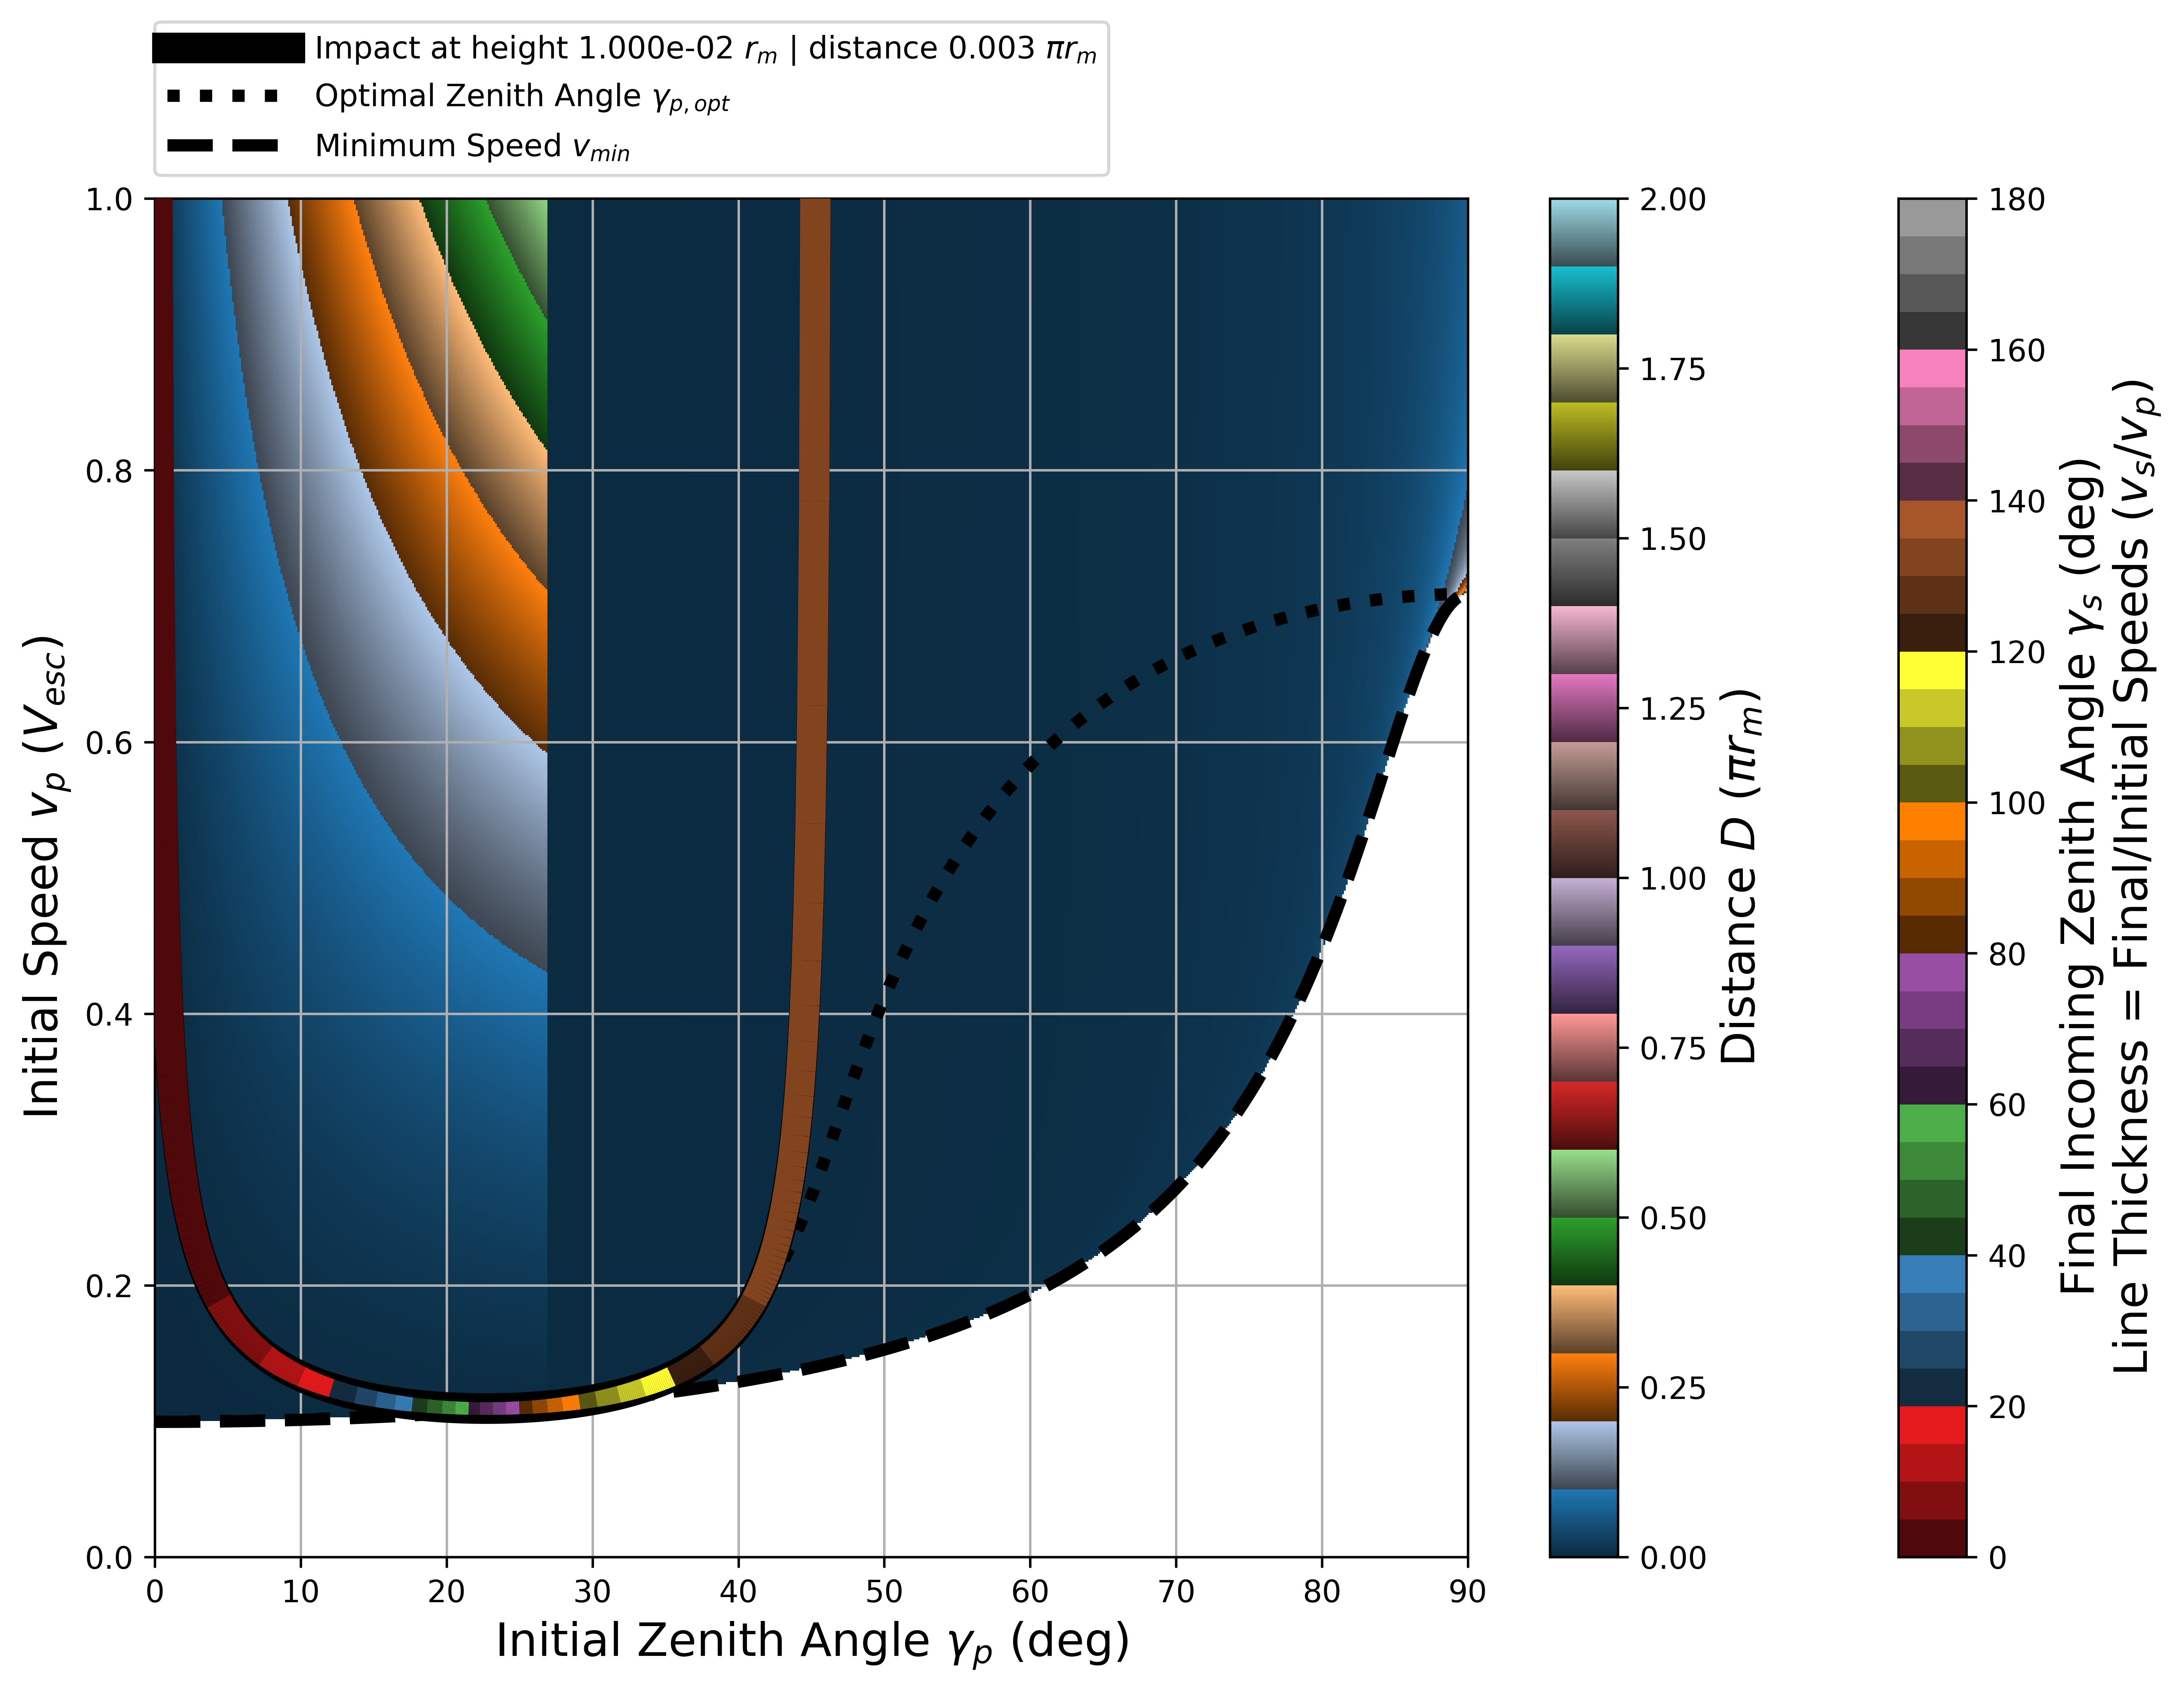
\includegraphics[width=1.00\linewidth]{dist_speed_zenith_plot_010_1.000e-02_0.010.png}
	\caption{The initial speed $v_p$ vs.\ initial zenith angle $\gamma_p$ as a function of distance $D$ is shown with a distance contour line at $0.003\pi r_m$ with a point-asset altitude of $0.01 r_m$. The contour line's color depicts the final incomming zenith angle $\gamma_s$ where the thickness of the line gives the ratio of the final and initial speeds $v_s/v_p$. The intersection of the distance contour line and the black dotted line gives the optimal zenith angle $\gamma_{p,opt}$ (Equation~
		\eqref{eq:gamma p ap 1}), i.e.\ the slowest initial speed to reach the contour line distance of $0.003\pi r_m$. The black dashed line gives the minimum achievable initial speed $v_{p,min}$ for a particular initial zenith angle (Equation \eqref{eq:vpmin}). The intersection of the distance contour line and $v_{p,min}$ occurs when the final incoming zenith angle $\gamma_s = 90^\circ$ (i.e., parallel to the local horizon) and marks a branch cut to another branch. The branch to the left of the branch cut are all ejecta hitting the point-asset above the local horizon, whereas the branch to the right are all ejecta hitting below the local horizon.}\label{fig:dist_speed_zenith_plot_010_1.000e-02_0.010}
\end{figure}

\begin{figure}[!htb]
	\centering
	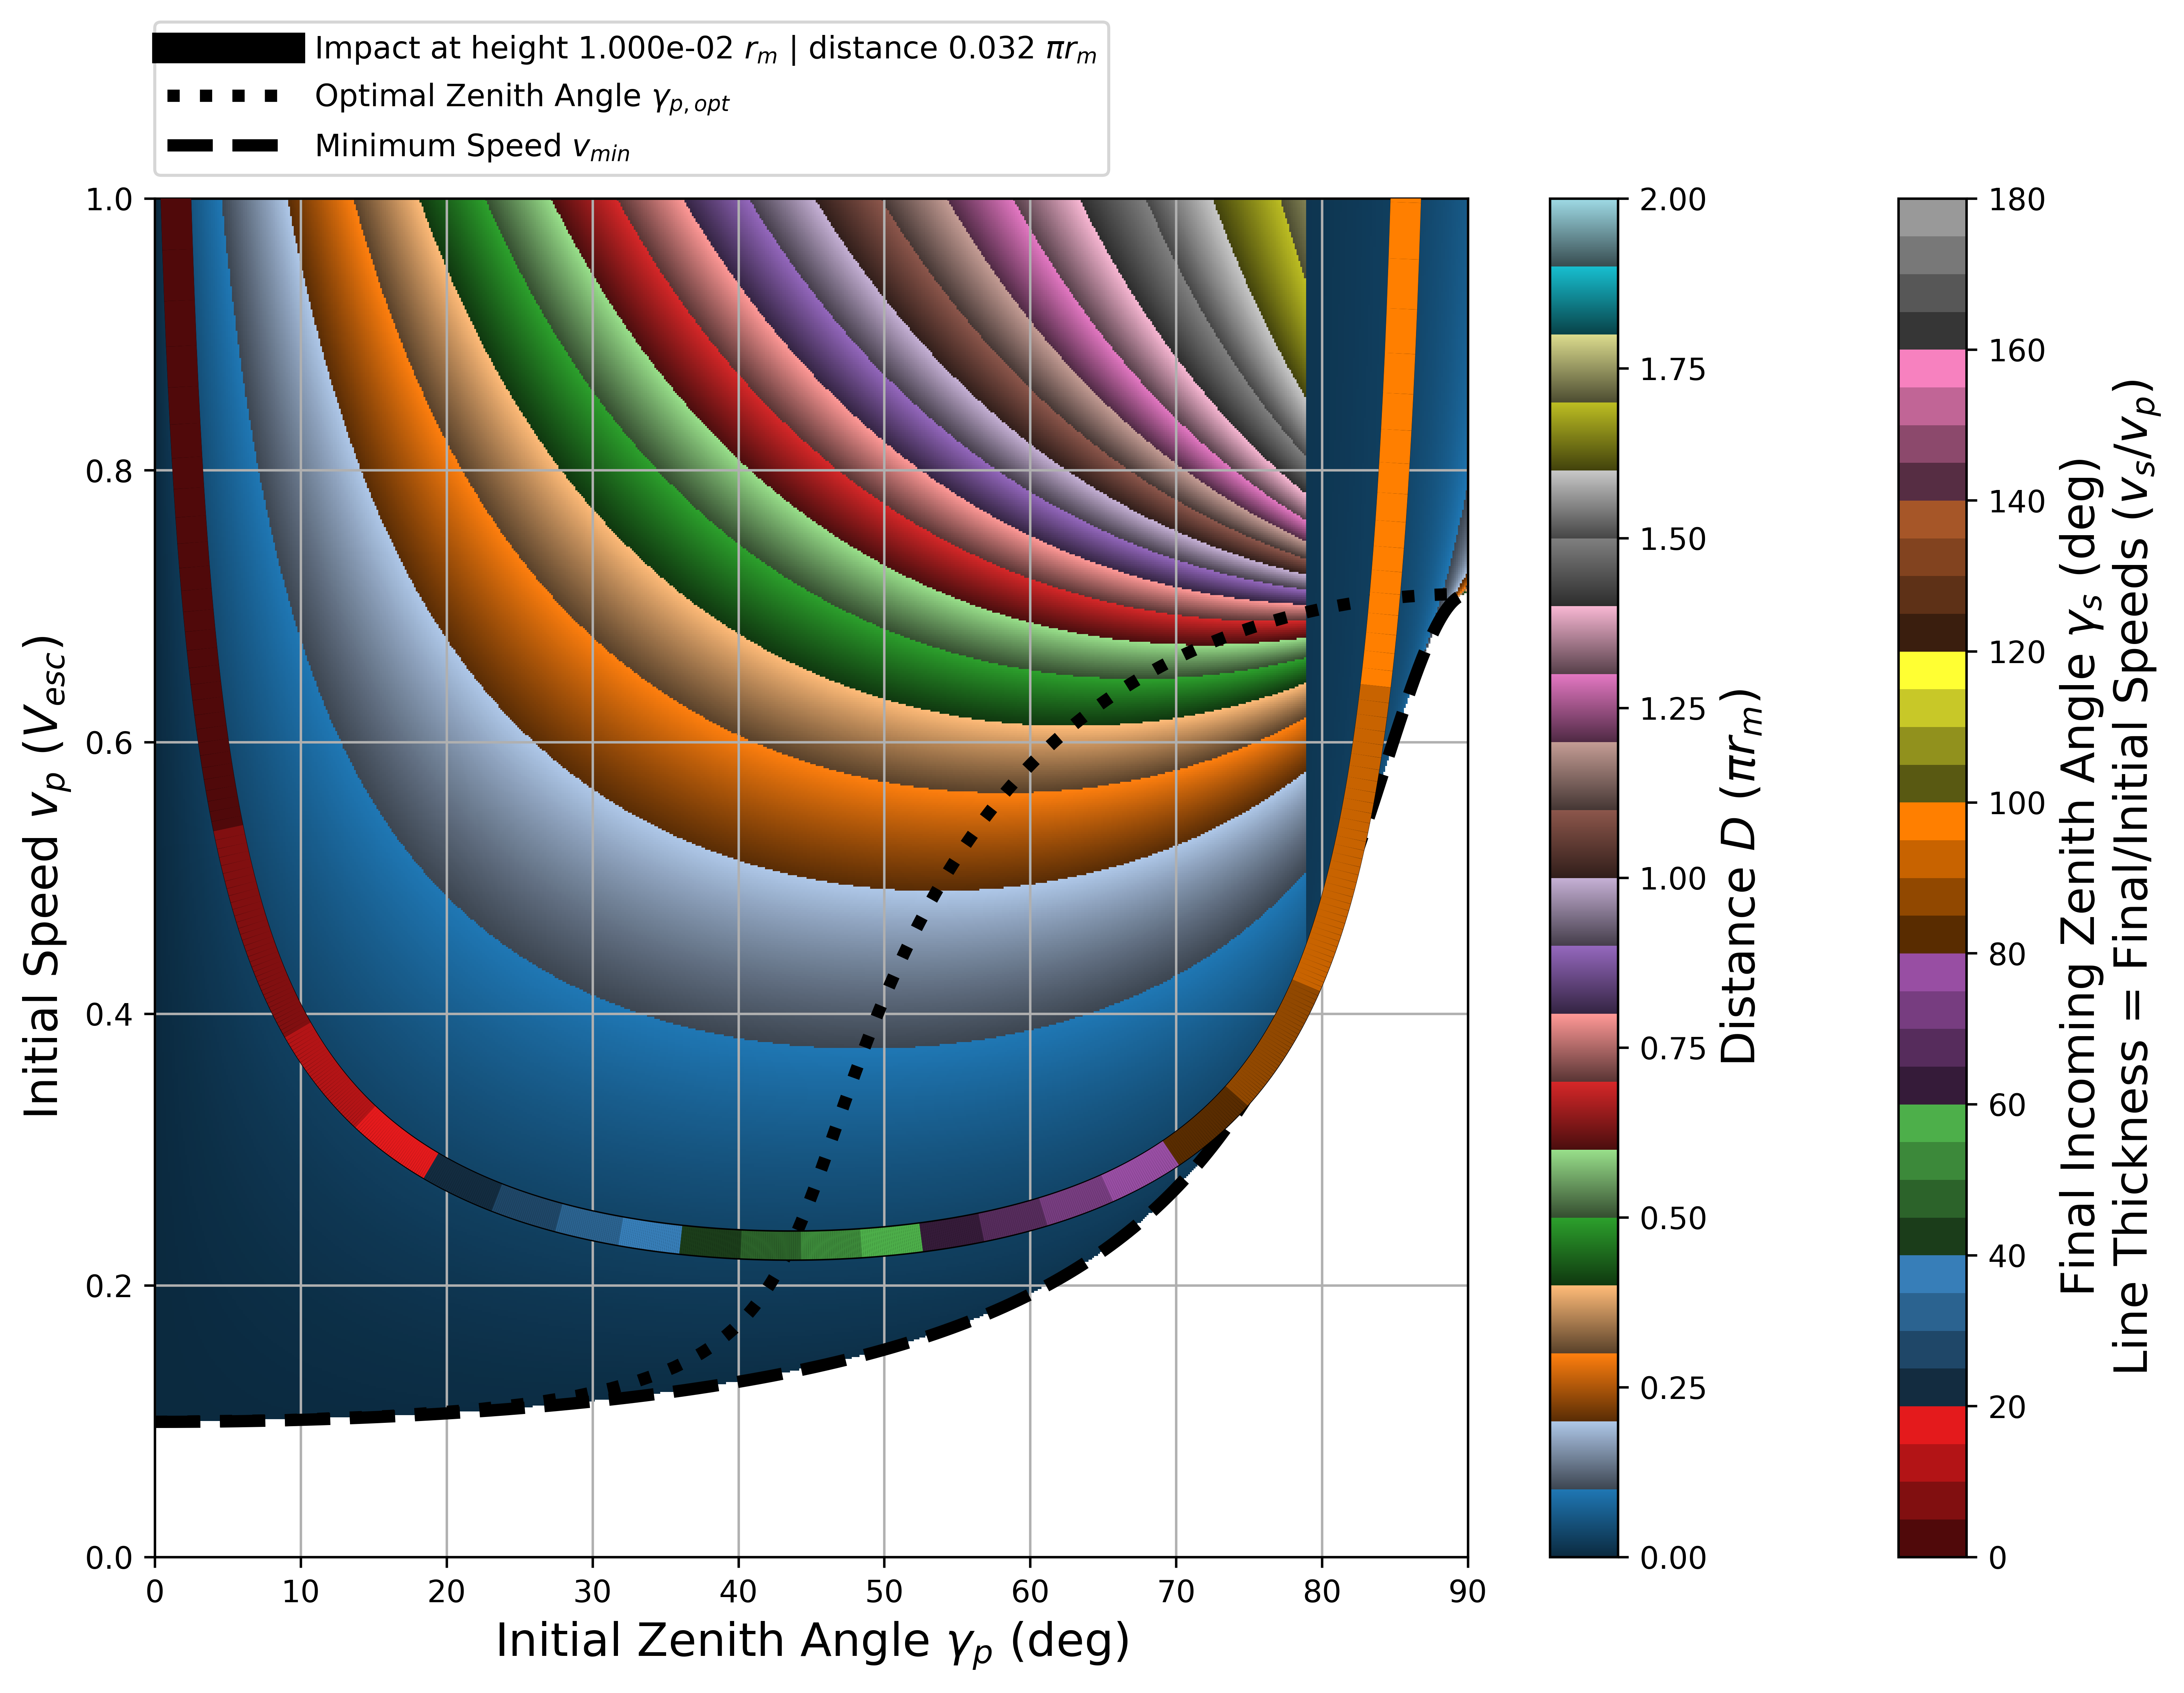
\includegraphics[width=1.00\linewidth]{dist_speed_zenith_plot_011_1.000e-02_0.100.png}
	\caption{The initial speed $v_p$ vs.\ initial zenith angle $\gamma_p$ as a function of distance $D$ is shown with a distance contour line at $0.032\pi r_m$ with a point-asset altitude of $0.01 r_m$. The contour line's color depicts the final incomming zenith angle $\gamma_s$ where the thickness of the line gives the ratio of the final and initial speeds $v_s/v_p$. The intersection of the distance contour line and the black dotted line gives the optimal zenith angle $\gamma_{p,opt}$ (Equation~
		\eqref{eq:gamma p ap 1}), i.e.\ the slowest initial speed to reach the contour line distance of $0.032\pi r_m$. The black dashed line gives the minimum achievable initial speed $v_{p,min}$ for a particular initial zenith angle (Equation \eqref{eq:vpmin}). The intersection of the distance contour line and $v_{p,min}$ occurs when the final incoming zenith angle $\gamma_s = 90^\circ$ (i.e., parallel to the local horizon) and marks a branch cut to another branch. The branch to the left of the branch cut are all ejecta hitting the point-asset above the local horizon, whereas the branch to the right are all ejecta hitting below the local horizon.}\label{fig:dist_speed_zenith_plot_011_1.000e-02_0.100}
\end{figure}

\begin{figure}[!htb]
	\centering
	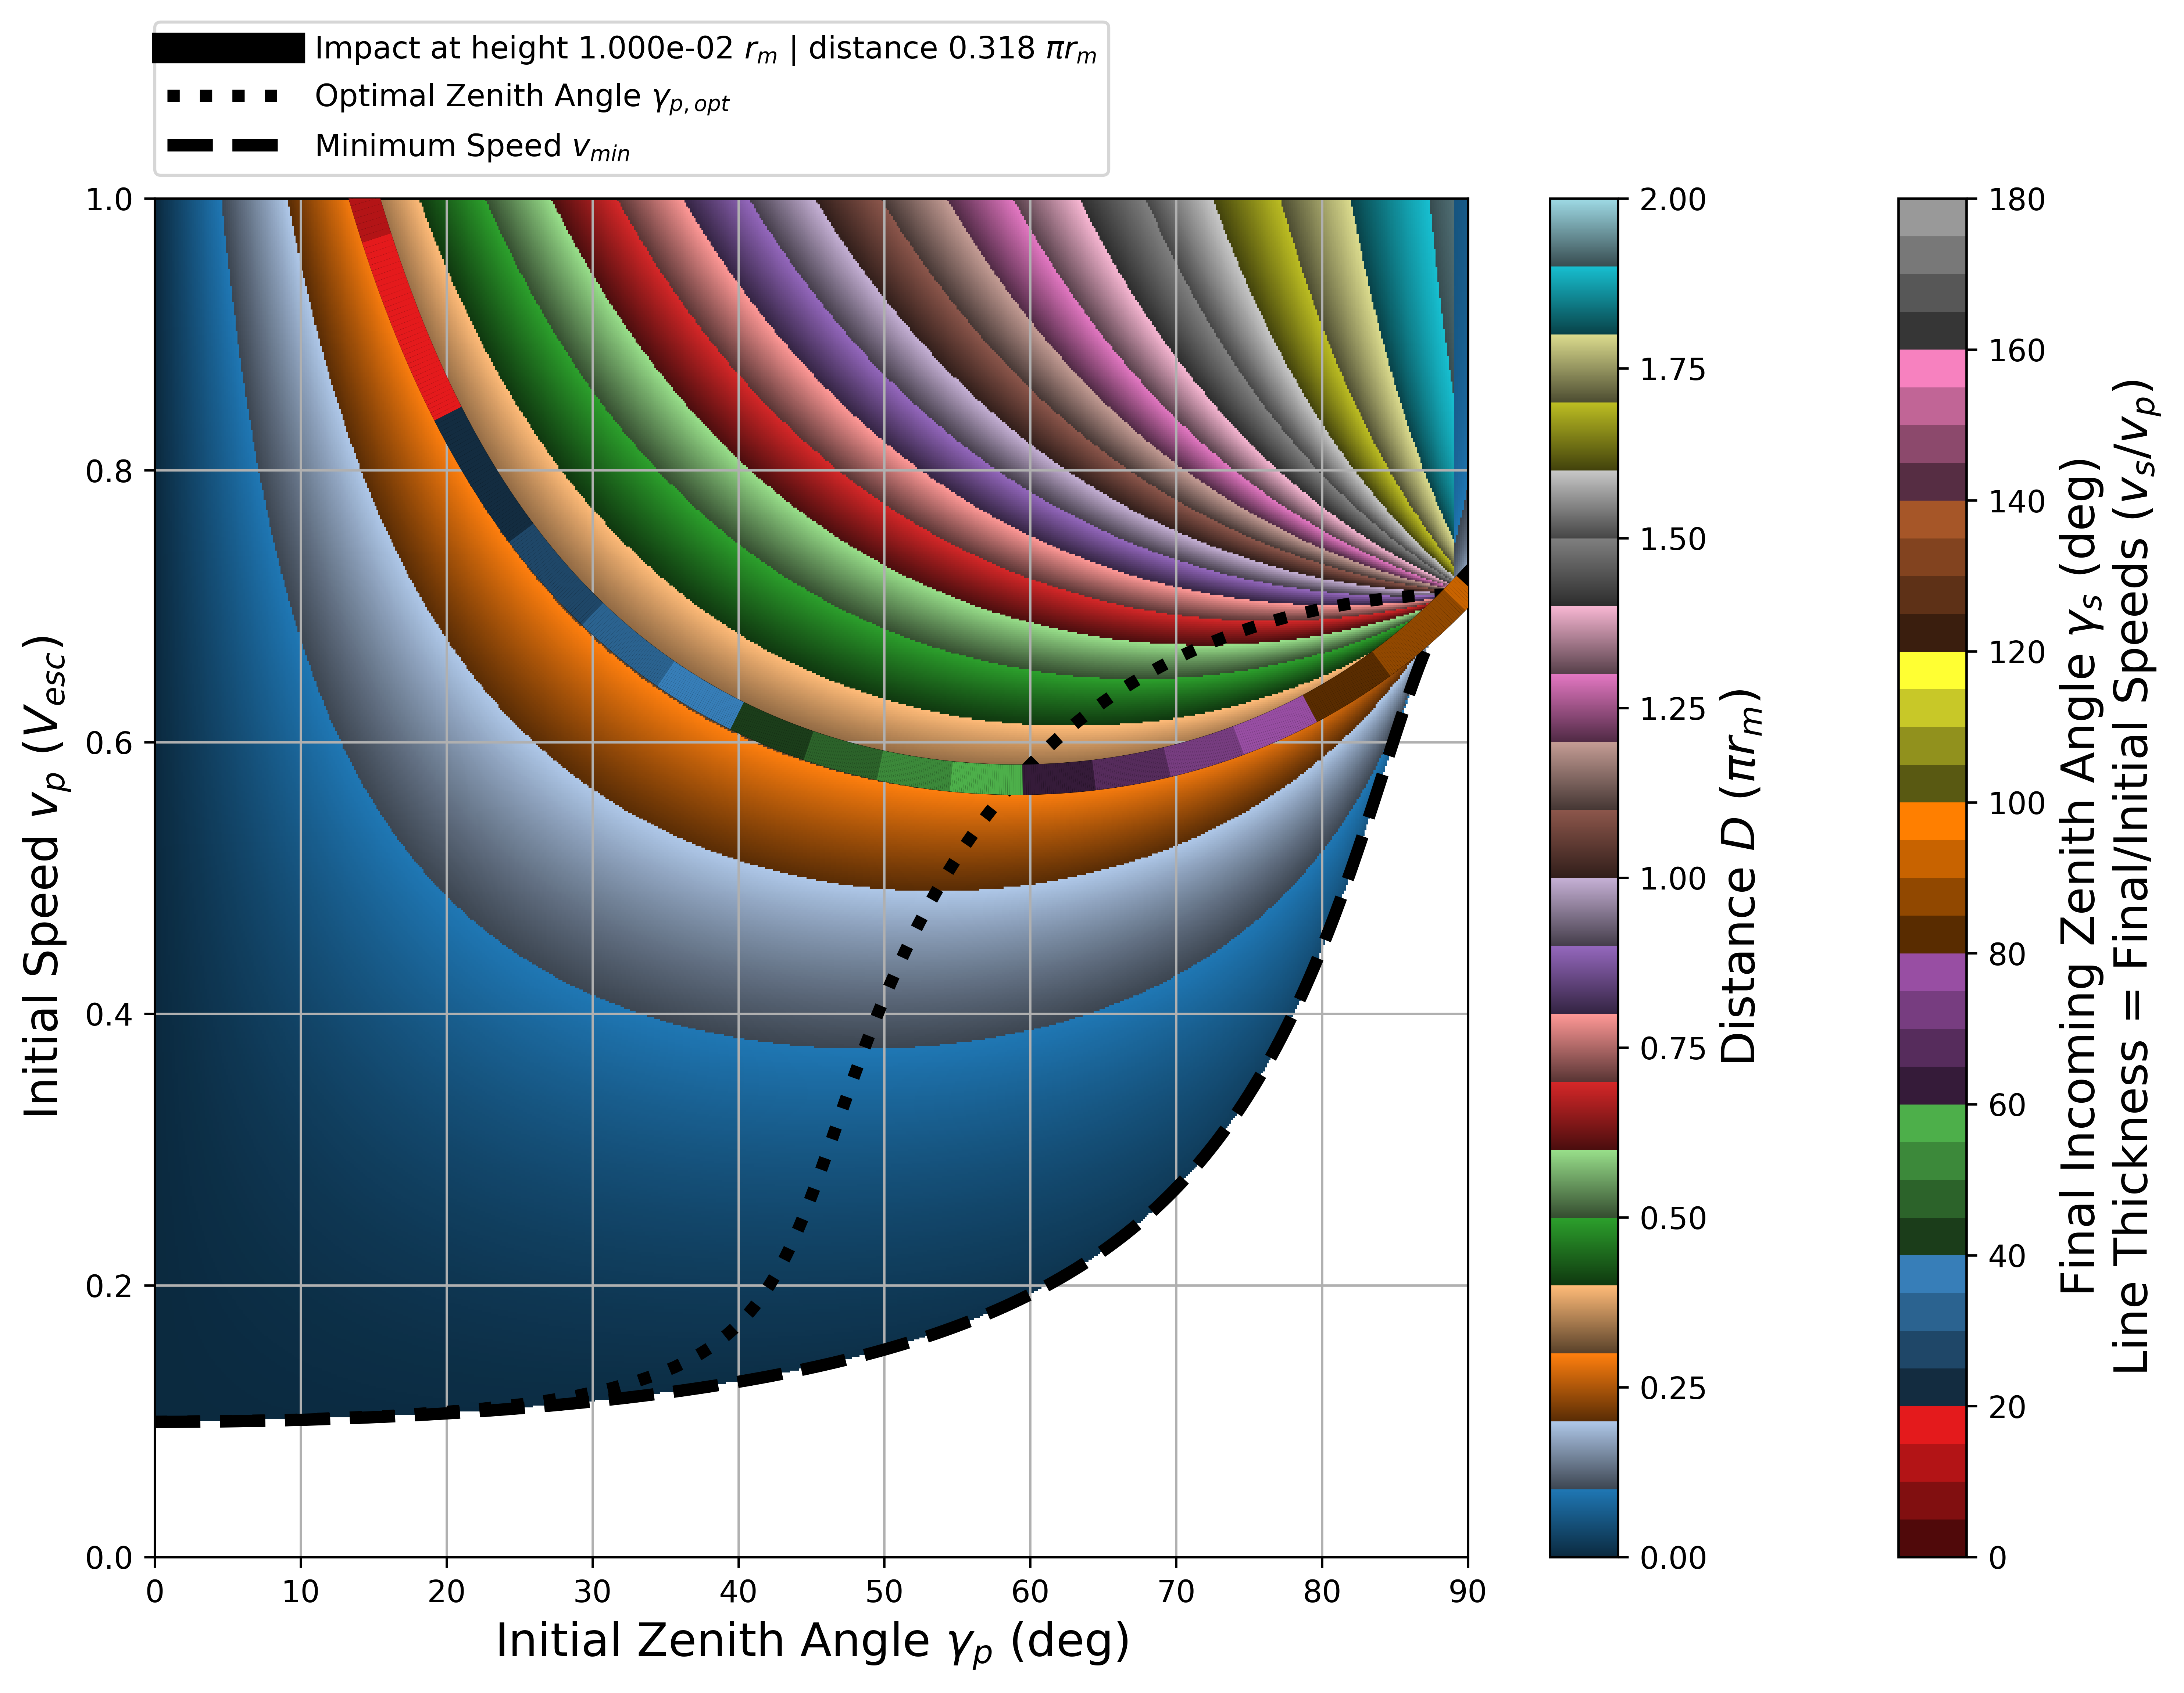
\includegraphics[width=1.0\linewidth]{dist_speed_zenith_plot_012_1.000e-02_1.000.png}
	\caption{The initial speed $v_p$ vs.\ initial zenith angle $\gamma_p$ as a function of distance $D$ is shown with a distance contour line at $0.318\pi r_m$ with a point-asset altitude of $0.01 r_m$. The contour line's color depicts the final incomming zenith angle $\gamma_s$ where the thickness of the line gives the ratio of the final and initial speeds $v_s/v_p$. The intersection of the distance contour line and the black dotted line gives the optimal zenith angle $\gamma_{p,opt}$ (Equation~
		\eqref{eq:gamma p ap 1}), i.e.\ the slowest initial speed to reach the contour line distance of $0.318\pi r_m$. The black dashed line gives the minimum achievable initial speed $v_{p,min}$ for a particular initial zenith angle (Equation \eqref{eq:vpmin}). The intersection of the distance contour line and $v_{p,min}$ occurs when the final incoming zenith angle $\gamma_s = 90^\circ$ (i.e., parallel to the local horizon) and marks a branch cut to another branch. The branch to the left of the branch cut are all ejecta hitting the point-asset above the local horizon, whereas the branch to the right are all ejecta hitting below the local horizon.}\label{fig:dist_speed_zenith_plot_012_1.000e-02_1.000}
\end{figure}

\begin{figure}[!htb]
	\centering
	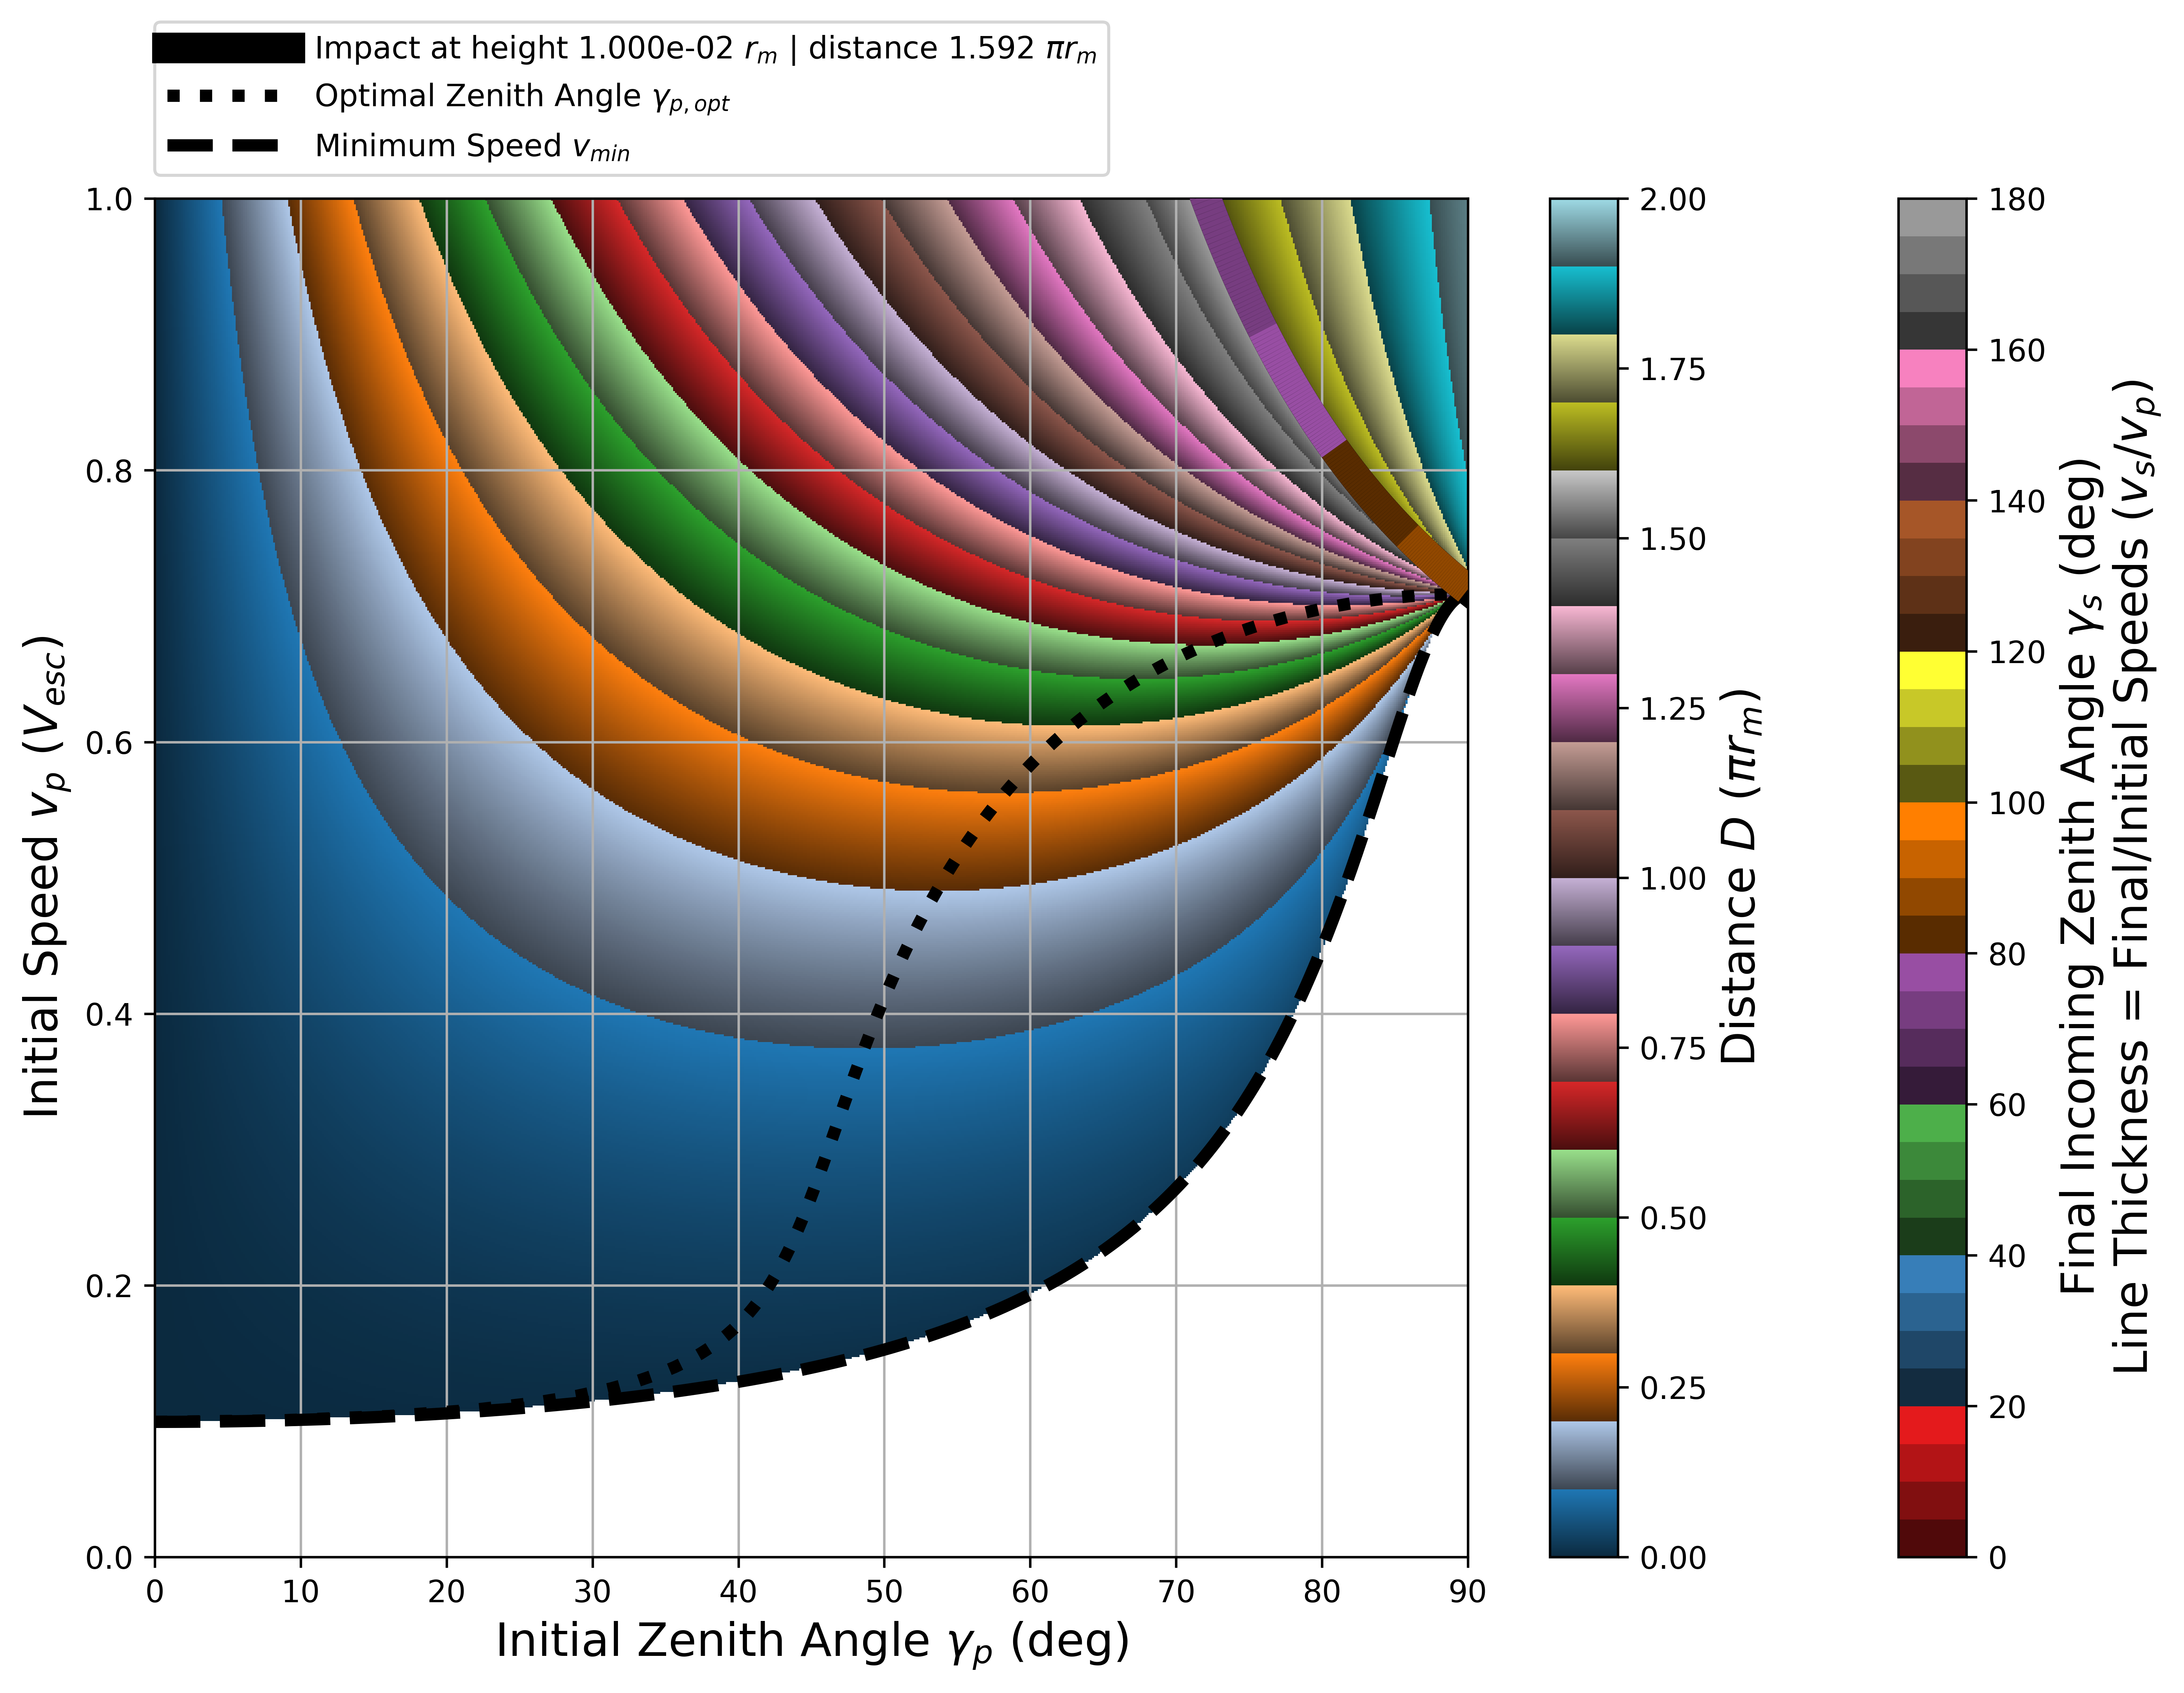
\includegraphics[width=1.0\linewidth]{dist_speed_zenith_plot_013_1.000e-02_5.000.png}
	\caption{The initial speed $v_p$ vs.\ initial zenith angle $\gamma_p$ as a function of distance $D$ is shown with a distance contour line at $1.592\pi r_m$ with a point-asset altitude of $0.01 r_m$. The contour line's color depicts the final incomming zenith angle $\gamma_s$ where the thickness of the line gives the ratio of the final and initial speeds $v_s/v_p$. The intersection of the distance contour line and the black dotted line gives the optimal zenith angle $\gamma_{p,opt}$ (Equation~
		\eqref{eq:gamma p ap 1}), i.e.\ the slowest initial speed to reach the contour line distance of $1.592\pi r_m$. The black dashed line gives the minimum achievable initial speed $v_{p,min}$ for a particular initial zenith angle (Equation \eqref{eq:vpmin}). The intersection of the distance contour line and $v_{p,min}$ occurs when the final incoming zenith angle $\gamma_s = 90^\circ$ (i.e., parallel to the local horizon) and marks a branch cut to another branch. The branch to the left of the branch cut are all ejecta hitting the point-asset above the local horizon, whereas the branch to the right are all ejecta hitting below the local horizon.}\label{fig:dist_speed_zenith_plot_013_1.000e-02_5.000}
\end{figure}


%%%%%

\begin{figure}[!htb]
	\centering
	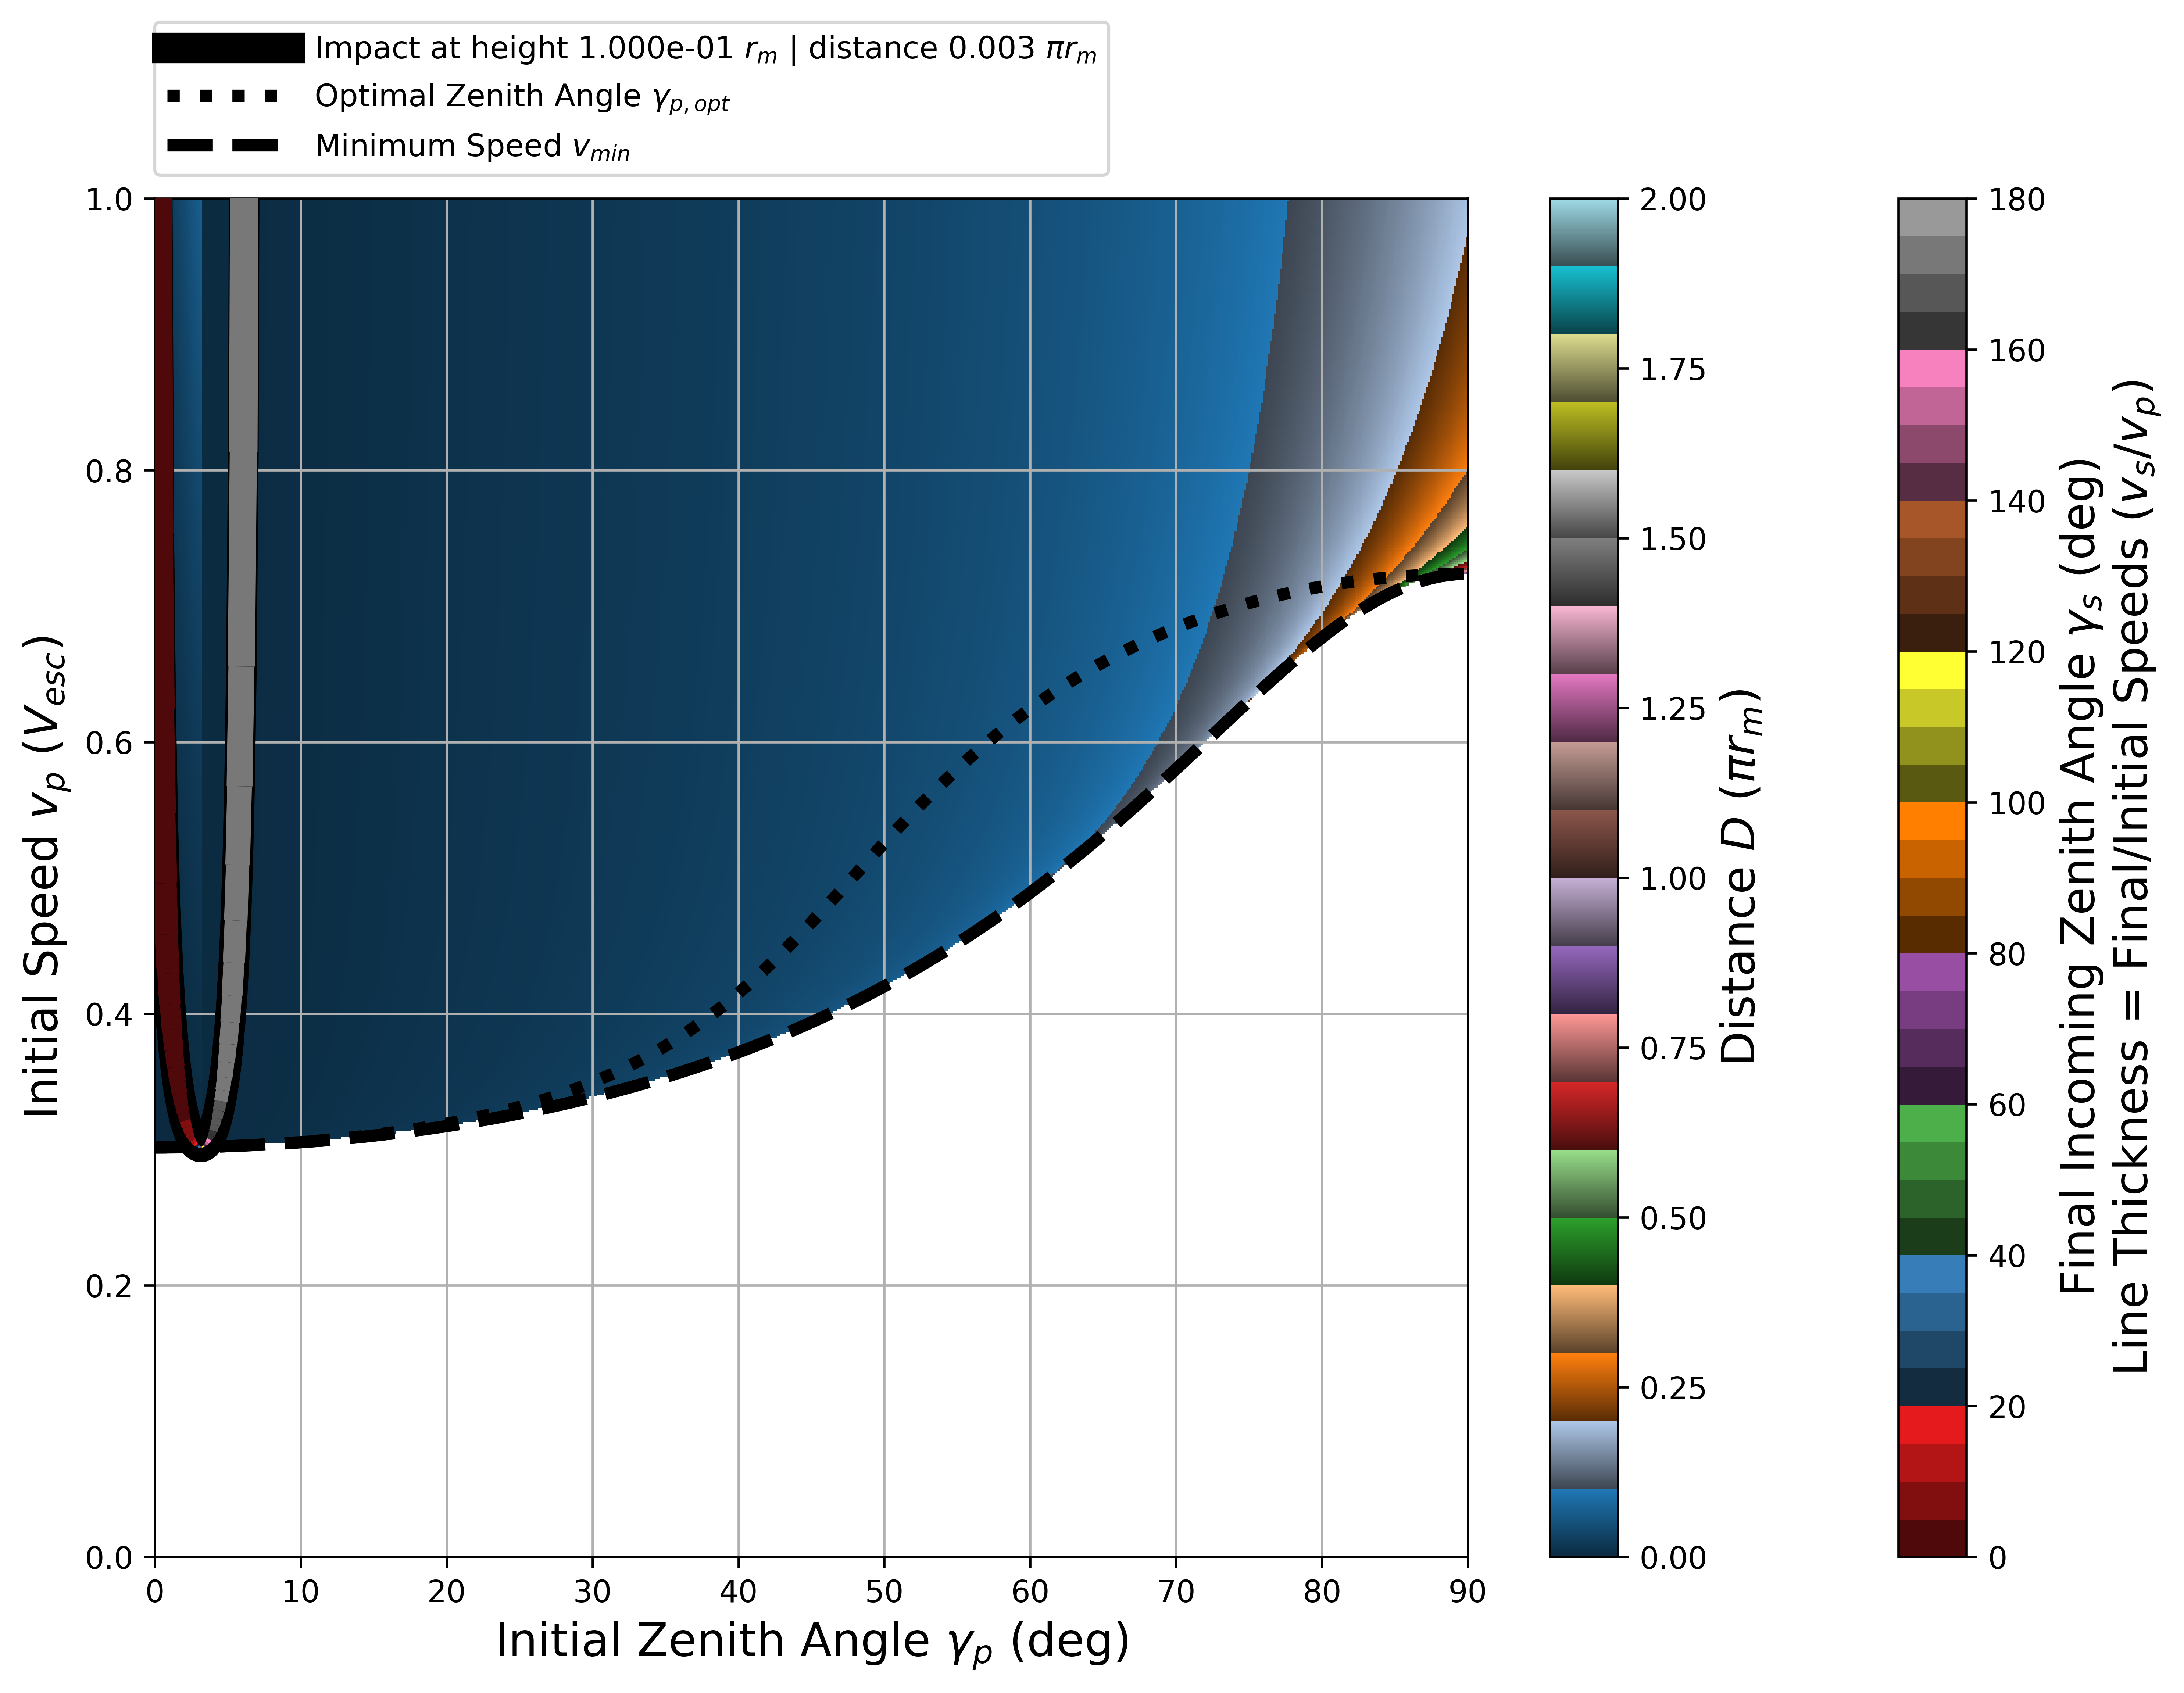
\includegraphics[width=1.0\linewidth]{dist_speed_zenith_plot_020_1.000e-01_0.010.png}
	\caption{The initial speed $v_p$ vs.\ initial zenith angle $\gamma_p$ as a function of distance $D$ is shown with a distance contour line at $0.003\pi r_m$ with a point-asset altitude of $0.1 r_m$. The contour line's color depicts the final incomming zenith angle $\gamma_s$ where the thickness of the line gives the ratio of the final and initial speeds $v_s/v_p$. The intersection of the distance contour line and the black dotted line gives the optimal zenith angle $\gamma_{p,opt}$ (Equation~
		\eqref{eq:gamma p ap 1}), i.e.\ the slowest initial speed to reach the contour line distance of $0.003\pi r_m$. The black dashed line gives the minimum achievable initial speed $v_{p,min}$ for a particular initial zenith angle (Equation \eqref{eq:vpmin}). The intersection of the distance contour line and $v_{p,min}$ occurs when the final incoming zenith angle $\gamma_s = 90^\circ$ (i.e., parallel to the local horizon) and marks a branch cut to another branch. The branch to the left of the branch cut are all ejecta hitting the point-asset above the local horizon, whereas the branch to the right are all ejecta hitting below the local horizon.}\label{fig:dist_speed_zenith_plot_020_1.000e-01_0.010}
\end{figure}

\begin{figure}[!htb]
	\centering
	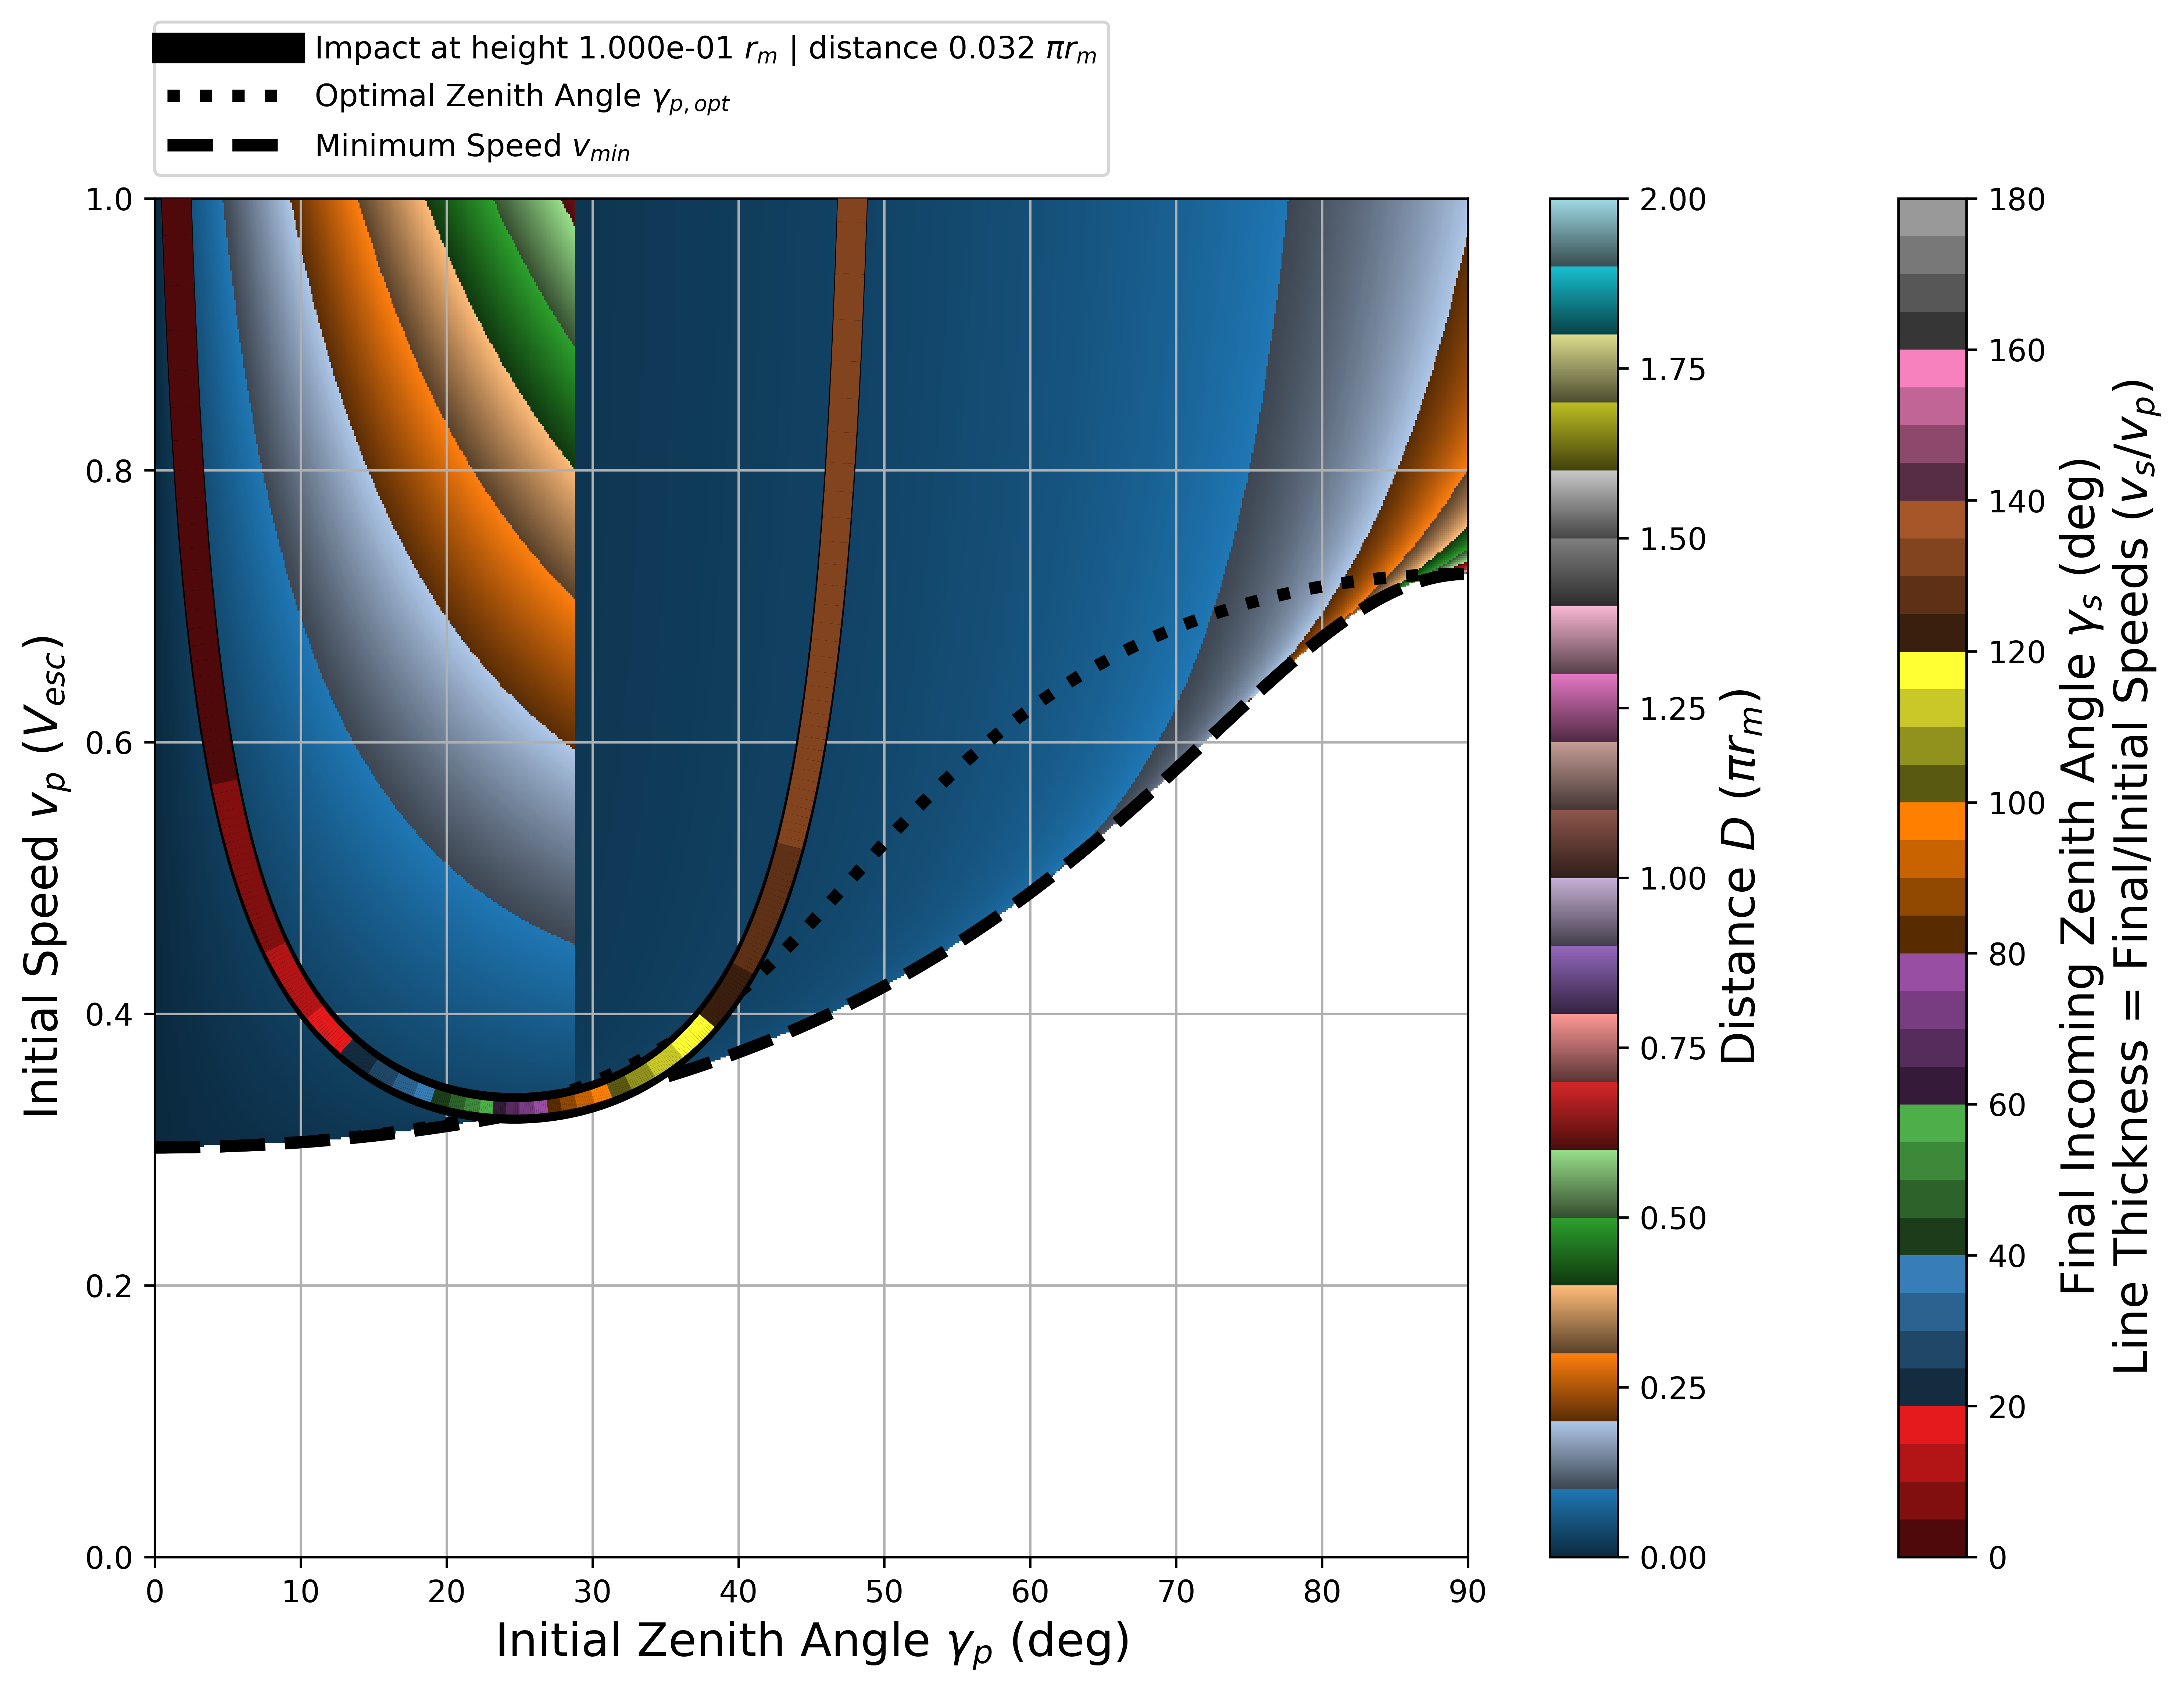
\includegraphics[width=1.0\linewidth]{dist_speed_zenith_plot_021_1.000e-01_0.100.png}
	\caption{The initial speed $v_p$ vs.\ initial zenith angle $\gamma_p$ as a function of distance $D$ is shown with a distance contour line at $0.032\pi r_m$ with a point-asset altitude of $0.1 r_m$. The contour line's color depicts the final incomming zenith angle $\gamma_s$ where the thickness of the line gives the ratio of the final and initial speeds $v_s/v_p$. The intersection of the distance contour line and the black dotted line gives the optimal zenith angle $\gamma_{p,opt}$ (Equation~
		\eqref{eq:gamma p ap 1}), i.e.\ the slowest initial speed to reach the contour line distance of $0.032\pi r_m$. The black dashed line gives the minimum achievable initial speed $v_{p,min}$ for a particular initial zenith angle (Equation \eqref{eq:vpmin}). The intersection of the distance contour line and $v_{p,min}$ occurs when the final incoming zenith angle $\gamma_s = 90^\circ$ (i.e., parallel to the local horizon) and marks a branch cut to another branch. The branch to the left of the branch cut are all ejecta hitting the point-asset above the local horizon, whereas the branch to the right are all ejecta hitting below the local horizon.}\label{fig:dist_speed_zenith_plot_021_1.000e-01_0.100}
\end{figure}

\begin{figure}[!htb]
	\centering
	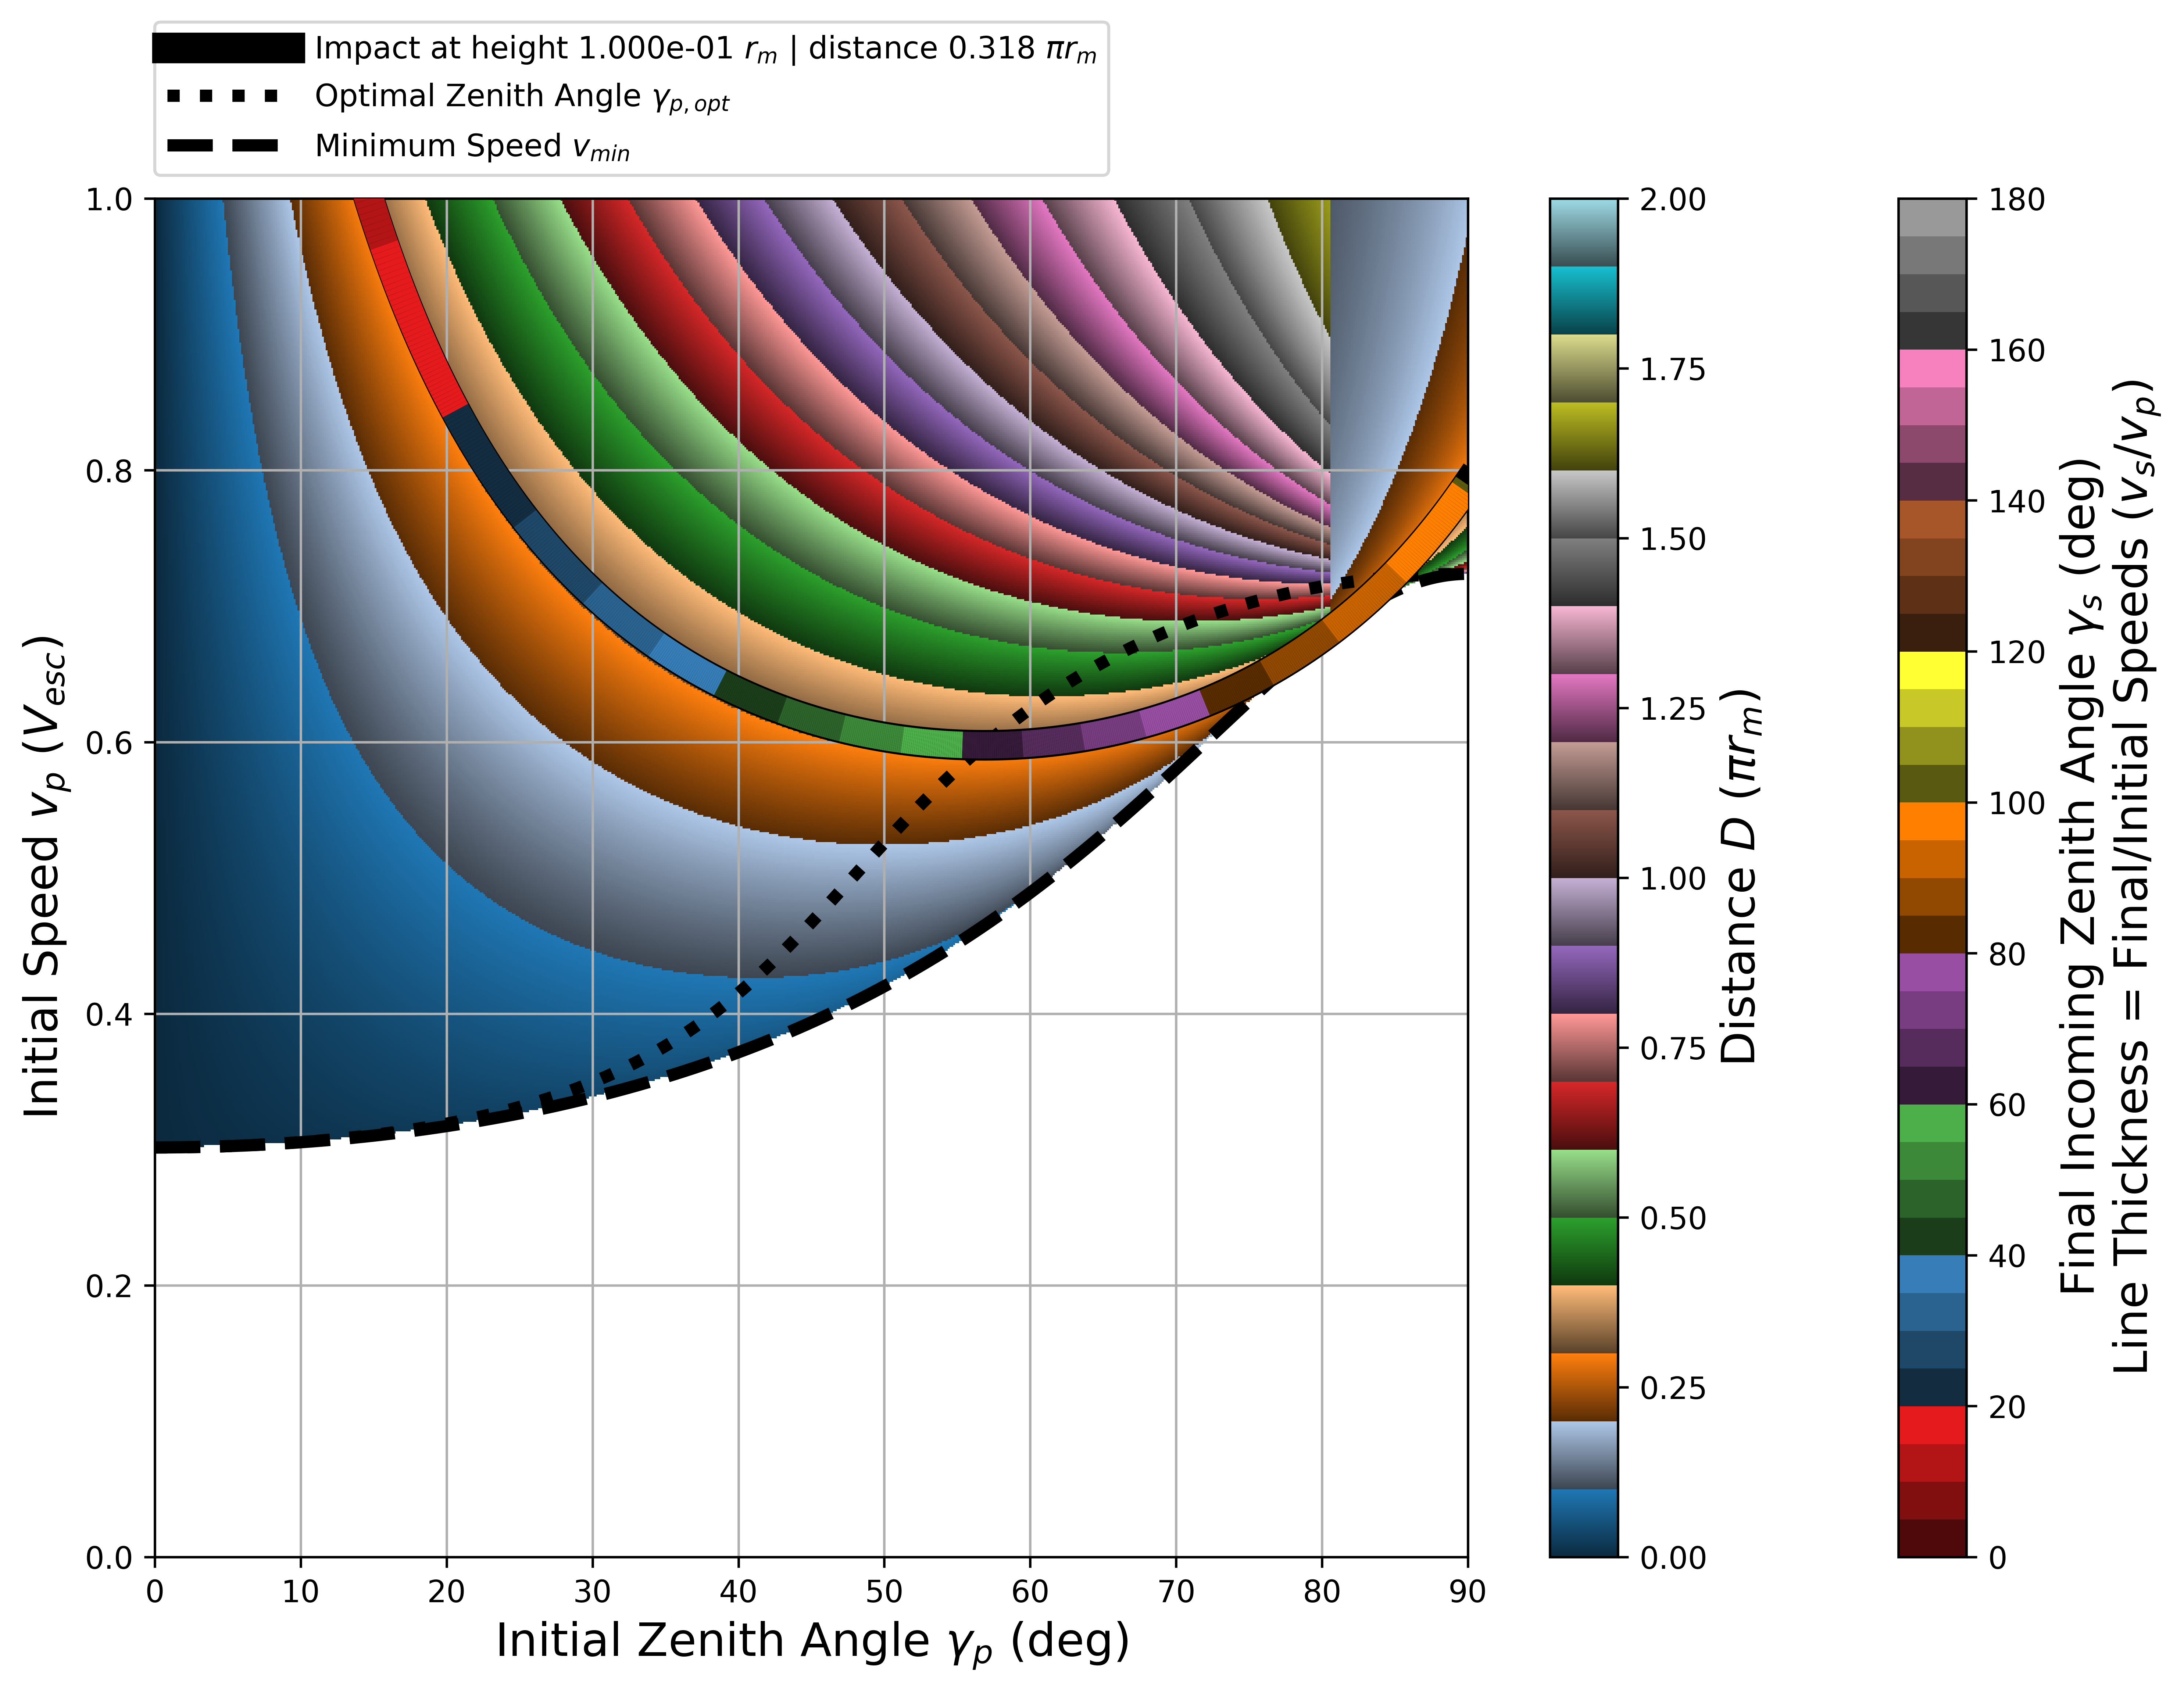
\includegraphics[width=1.0\linewidth]{dist_speed_zenith_plot_022_1.000e-01_1.000.png}
	\caption{The initial speed $v_p$ vs.\ initial zenith angle $\gamma_p$ as a function of distance $D$ is shown with a distance contour line at $0.318\pi r_m$ with a point-asset altitude of $0.1 r_m$. The contour line's color depicts the final incomming zenith angle $\gamma_s$ where the thickness of the line gives the ratio of the final and initial speeds $v_s/v_p$. The intersection of the distance contour line and the black dotted line gives the optimal zenith angle $\gamma_{p,opt}$ (Equation~
		\eqref{eq:gamma p ap 1}), i.e.\ the slowest initial speed to reach the contour line distance of $0.318\pi r_m$. The black dashed line gives the minimum achievable initial speed $v_{p,min}$ for a particular initial zenith angle (Equation \eqref{eq:vpmin}). The intersection of the distance contour line and $v_{p,min}$ occurs when the final incoming zenith angle $\gamma_s = 90^\circ$ (i.e., parallel to the local horizon) and marks a branch cut to another branch. The branch to the left of the branch cut are all ejecta hitting the point-asset above the local horizon, whereas the branch to the right are all ejecta hitting below the local horizon.}\label{fig:dist_speed_zenith_plot_022_1.000e-01_1.000}
\end{figure}

\begin{figure}[!htb]
	\centering
	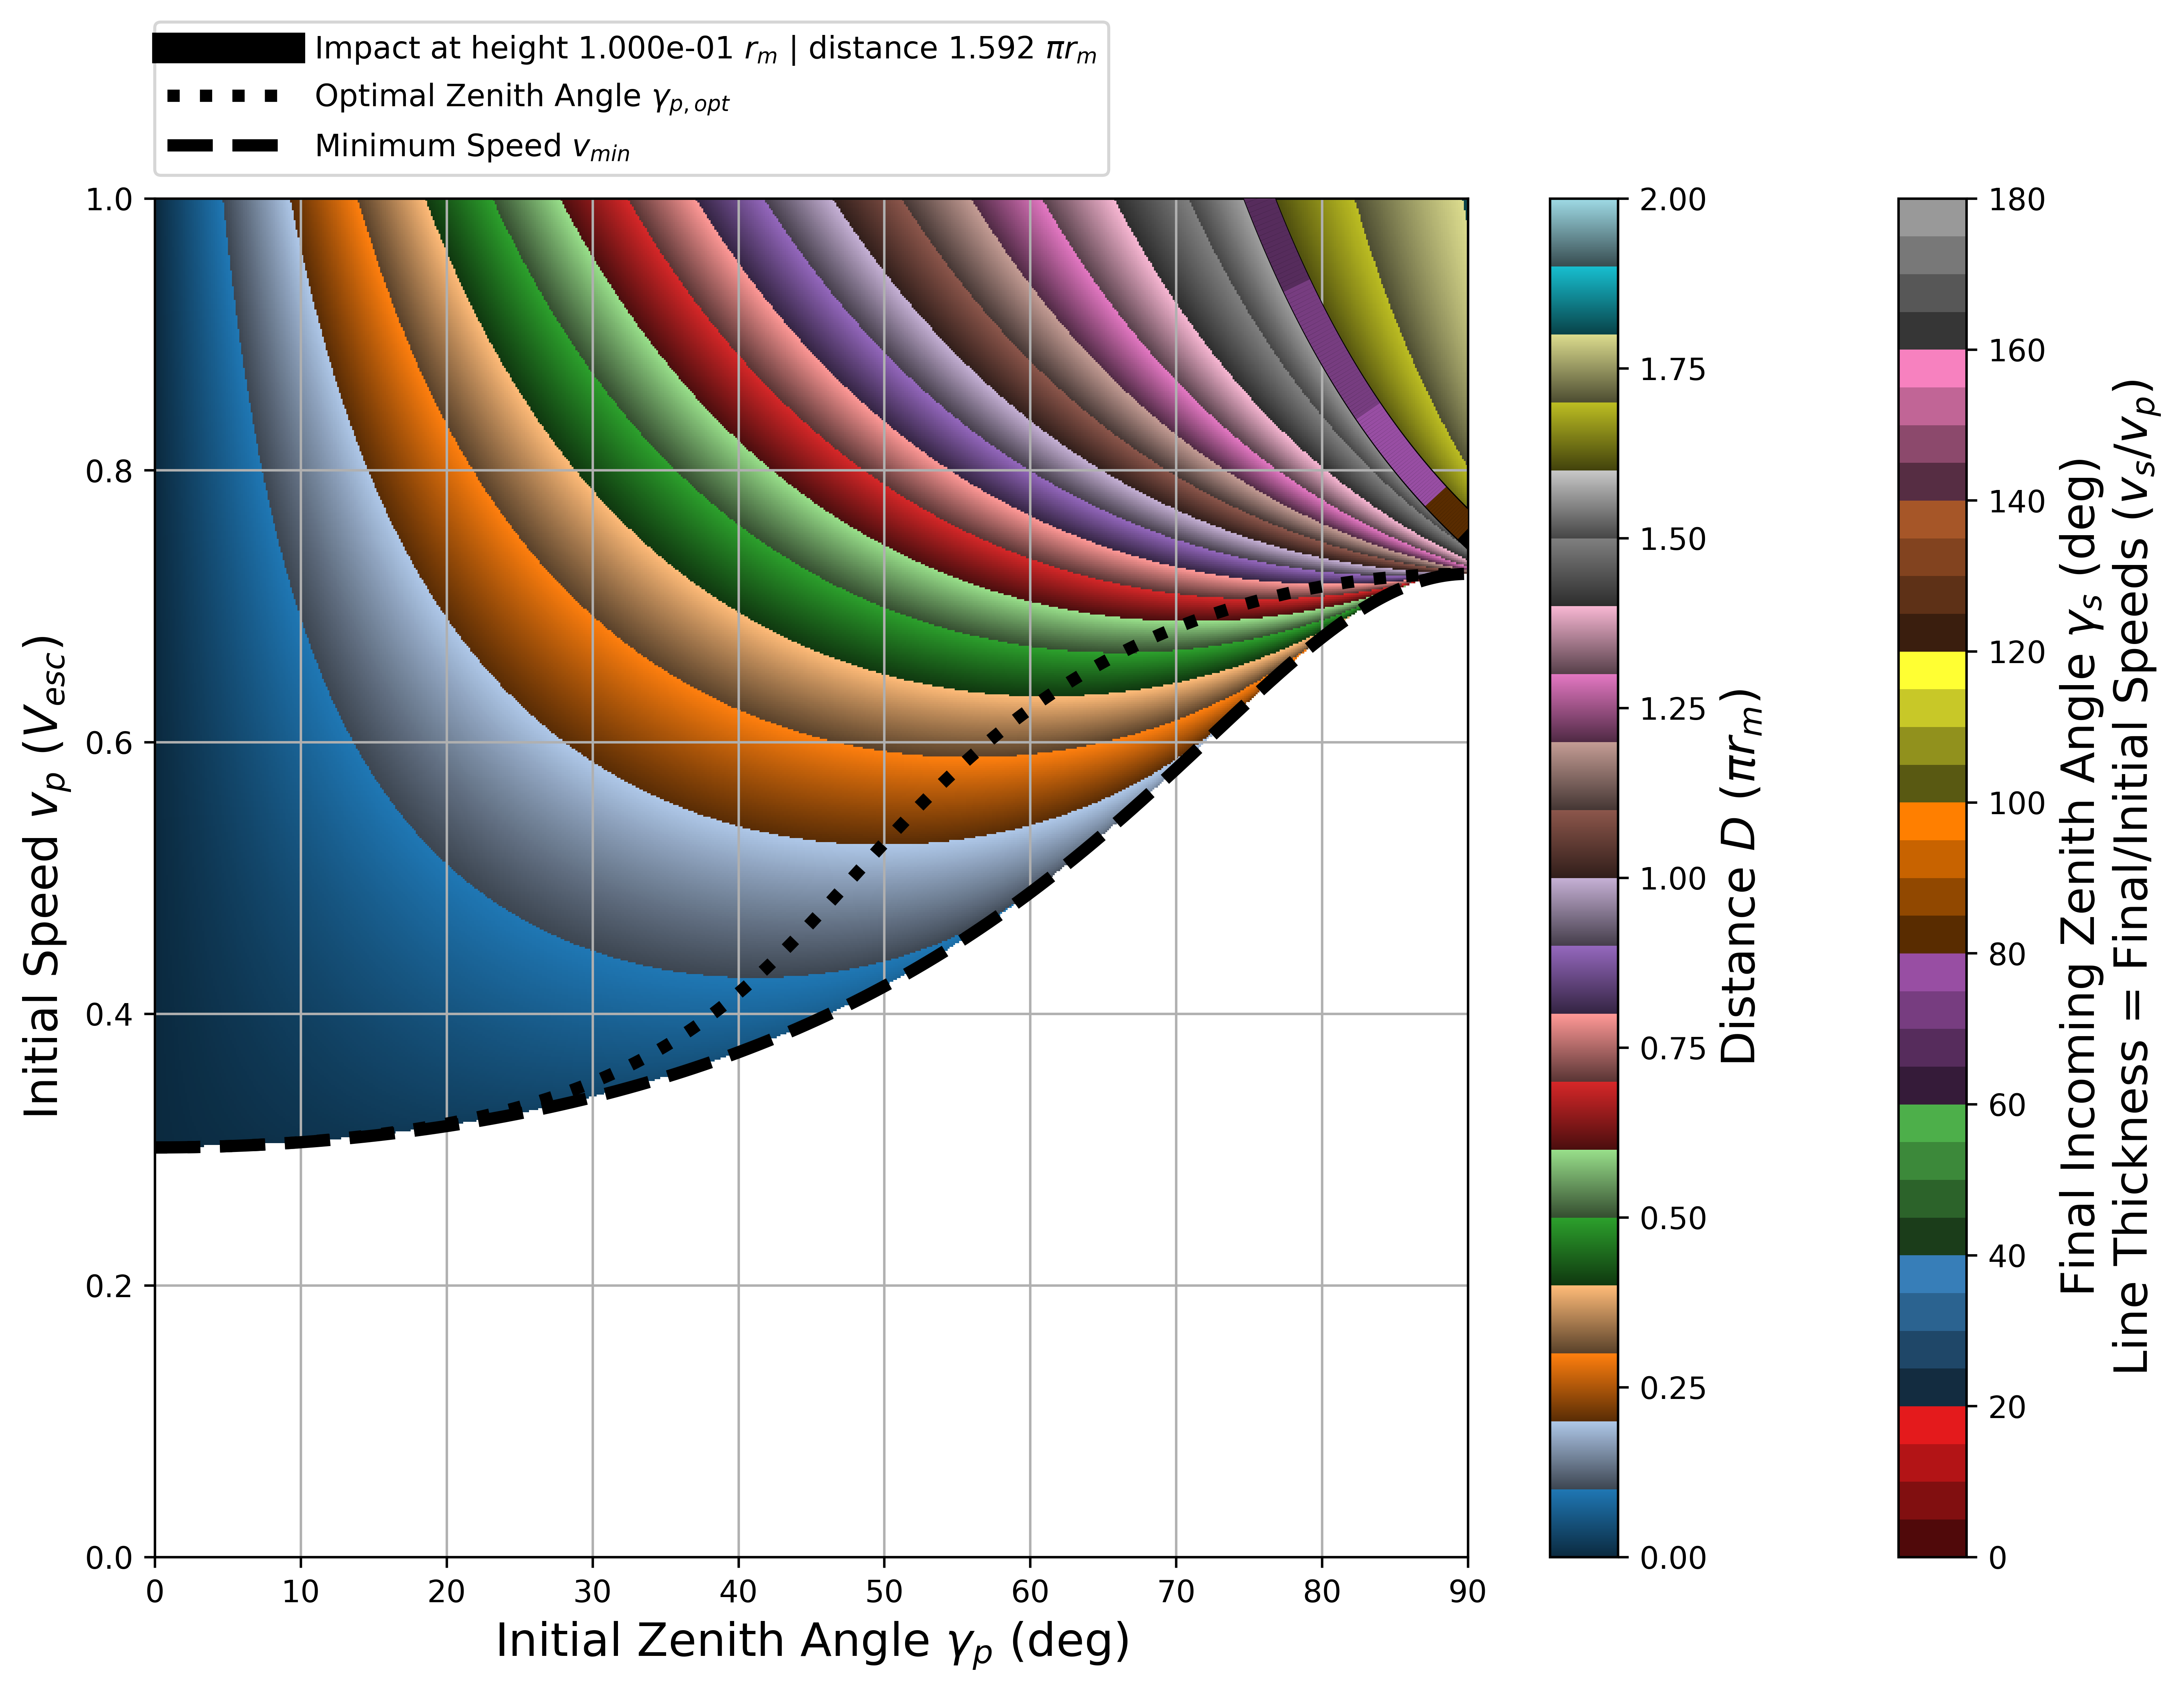
\includegraphics[width=1.0\linewidth]{dist_speed_zenith_plot_023_1.000e-01_5.000.png}
	\caption{The initial speed $v_p$ vs.\ initial zenith angle $\gamma_p$ as a function of distance $D$ is shown with a distance contour line at $1.592\pi r_m$ with a point-asset altitude of $0.1 r_m$. The contour line's color depicts the final incomming zenith angle $\gamma_s$ where the thickness of the line gives the ratio of the final and initial speeds $v_s/v_p$. The intersection of the distance contour line and the black dotted line gives the optimal zenith angle $\gamma_{p,opt}$ (Equation~
		\eqref{eq:gamma p ap 1}), i.e.\ the slowest initial speed to reach the contour line distance of $1.592\pi r_m$. The black dashed line gives the minimum achievable initial speed $v_{p,min}$ for a particular initial zenith angle (Equation \eqref{eq:vpmin}). The intersection of the distance contour line and $v_{p,min}$ occurs when the final incoming zenith angle $\gamma_s = 90^\circ$ (i.e., parallel to the local horizon) and marks a branch cut to another branch. The branch to the left of the branch cut are all ejecta hitting the point-asset above the local horizon, whereas the branch to the right are all ejecta hitting below the local horizon.}\label{fig:dist_speed_zenith_plot_023_1.000e-01_5.000}
\end{figure}

\clearpage


%%%%%%%%%%%%%%%%%%%%%%%%%%%%%%%%%%%%%%%%%%%%%%%%%%%%%%%%%%%%%%%%%%%%%%
\subsection{Azimuthal Field-of-View}\label{ssec:Azimuthal Field of View}

The field-of-view (FOV) of the asset from the crater, in terms of the azimuth, must be understood by spherical geometry. If the asset is assumed to be a cylinder with the base parallel to the local horizon, then the effective radius of the cylinder $a_i = c_i/1$ and the effective distance from the crater to the asset $D_i$ is modified from the line-of-sight radius and distance $a$ and $D$, respectively (see Figure \ref{fig:FOV}). The center of the asset is at point $\mathcal{O}$.

There is a special case when the crater is within the asset's antipode projection (Figure \ref{fig:FOV_antipode}). The effective radius $a_i$ becomes $a_i = (a_{0,i} + a_{1,i})/2$ with the effective distance $D_i$, not shown in the figure. Both the asset and asset antipode are superimposed on each other, also showing the crater $\mathcal{C}$ and crater antipode $\mathcal{C}_{antipode}$ points. 

% https://mirrors.mit.edu/CTAN/macros/latex/contrib/tkz/tkz-euclide/doc/tkz-euclide.pdf
\begin{figure}[!htb]
	\centering
	
	\begin{tikzpicture}[scale=2.6]
	\tkzDefPoint(-1,0){A}
	\tkzDefPoint(1,0){A2}
	\tkzLabelPoint[below right](A2){$\mathcal{D}$}
	\tkzDefPoint(0,0){B}
	\tkzLabelPoint[below](B){$\mathcal{O}$}
	\tkzLabelSegment[below](B,A2){$a$}
	
	\tkzDefPoint(4,0){C}
	\tkzLabelPoint[right](C){$\mathcal{C}$}
	%\tkzLabelSegment[below](C,A2){$D$}
	
	\tkzDrawSegment[dim={\(D\),-1cm,below=2mm},
	dim style/.append style={black,
		dash pattern={on 2pt off 2pt}}](A2,C)
	
	\tkzDefPoint(0.25, 0.9682){D}
	\tkzLabelPoint[above left](D){$\mathcal{E}$}
	
	
	\tkzDrawSegment[dim={\(D_{max}\),0.5cm,above=2mm},
	dim style/.append style={black,
		dash pattern={on 2pt off 2pt}}](D,C)
	
	\tkzDrawSegment(A,C)
	\tkzDrawSegment[dashed](D,C)
	\tkzDrawSegment[dashed](D,B)
	\tkzMarkRightAngle(B,D,C)
	%\tkzDrawSegment[dim={\(l_0\),1cm,right=2mm},
	%dim style/.append style={red,
	%	dash pattern={on 2pt off 2pt}}](A,C)
	\tkzDrawCircles(B,A)
	
	
	\tkzDefPoint(-1,0.5){A3}
	\tkzDrawSegment(A3,C)
	
	\tkzDefPoint(0.9524,0.304757){E1}
	\tkzDefPoint(-0.87322,0.4873){E2}
	\tkzLabelPoint[below](E2){$\mathcal{A}$}
	\tkzLabelPoint[left](E1){$\mathcal{B}$}
	%\tkzLabelPoints(E1, E2)
	
	\tkzMarkAngle[gray,size=0.15](B,E1,C)
	\tkzFindAngle(B,E1,C)
	\tkzLabelAngle[pos=0.2](B,E1,C){$\alpha_i$}
	\tkzFillAngle[fill=blue!20, opacity=0.5,size=0.15](B,E1,C)
	
	\tkzDefPoint(0,1){E3}
	\tkzDrawSegment(B,E3)
	\tkzMarkRightAngle(A2,B,E3)
	
	\tkzDrawSegment[dim={\(c_{i}\),-0.25cm,above=1mm},
	dim style/.append style={black,
		dash pattern={on 2pt off 2pt}}](E1,E2)
	
	
	\tkzDrawSegment[dim={\(D_{i}\),0.25cm,above=1mm},
	dim style/.append style={black,
		dash pattern={on 2pt off 2pt}}](E1,C)
	
	\tkzMarkAngle[gray,size=1.3](E2,C,B)
	\tkzFindAngle(E2,C,B)
	\tkzLabelAngle[pos=1.4](E2,C,B){$\beta_i$}
	\tkzFillAngle[fill=blue!20, opacity=0.5,size=1.3](E2,C,B)
	
	\tkzMarkAngle[gray,size=0.8](D,C,B)
	\tkzFindAngle(E2,C,B)
	\tkzLabelAngle[pos=1](D,C,B){$\beta_{max}$}
	\tkzFillAngle[fill=red!20, opacity=0.5,size=0.8](D,C,B)
	
	\tkzDrawSegment(B,E1)
	\tkzDrawSegment(B,E2)
	\tkzLabelSegment[below](B,E1){$a$}
	\tkzLabelSegment[below](B,E2){$a$}
	
	\tkzDrawPoints(E1,E2,C,A2,D)
	\end{tikzpicture}
	
	\caption{A bird's eye view of the asset (circle of radius $a$) and the crater location (point $\mathcal{C}$) projected on the surface of the Moon. The FOV the asset encompasses from the point of view of the crater is $2\beta_{max}$.}\label{fig:FOV}
\end{figure}


\begin{figure}[!htb]
	\centering
	
	\begin{tikzpicture}[scale=2.6]
	\tkzDefPoint(-1,0){A1}
	\tkzDefPoint(1,0){A2}
	\tkzDefPoint(0,0){B}
	\tkzDefPoint(0,1){B1}
	\tkzDefPoint(0,-1){B2}
	\tkzDrawCircles(B,A)
	\tkzLabelPoint[above left](B){$\mathcal{O}$}
	
	\tkzDrawSegment(A1,A2)
	\tkzDrawSegment(B1,B2)
	
	\tkzDefPoint(0,-0.8){C1}
	\tkzLabelPoint[above right](C1){$\mathcal{C}$}
	\tkzDefPoint(0,0.8){C2}
	\tkzLabelPoint[below right](C2){$\mathcal{C}_{antipode}$}
	
	\tkzDrawPoints(C1, C2, B)
	
	\tkzDefPoint(-0.1118, -0.9937){C1A}
	\tkzDefPoint(0.8047, 0.5937){C1B}
	
	\tkzDefPoint(0.1118, 0.9937){C2B}
	\tkzDefPoint(-0.8047, -0.5937){C2A}
	\tkzDrawSegment(C1A,C1B)
	\tkzDrawSegment(C2B,C2A)
	\tkzDrawSegment(C1A,B)
	\tkzDrawSegment(C1B,B)
	
	\tkzMarkAngle[gray,size=0.2](C1B,C1,B)
	\tkzFindAngle(C1B,C1,B)
	\tkzLabelAngle[pos=0.3](C1B,C1,B){$\beta_i$}
	\tkzFillAngle[fill=blue!20, opacity=0.5,size=0.2](C1B,C1,B)
	
	\tkzLabelSegment[left](B,C1A){$a$}
	\tkzLabelSegment[left](B,C1B){$a$}
	
	\tkzDrawSegment[dim={\(a_0\),-0.25cm,right=1mm},
	dim style/.append style={black,
		dash pattern={on 2pt off 2pt}}](B2,C1)
	
	%\tkzLabelSegment[right](B2,C1){$a_0$}
	\tkzLabelSegment[below right](C1,C1B){$a_{1,i}$}
	
	\tkzDrawSegment[dim={\(a_{0,i}\),0.25cm,left=1mm},
	dim style/.append style={black,
		dash pattern={on 2pt off 2pt}}](C1A,C1)
	
	\tkzDrawSegment[dim={\(a_{1,i}\),0.25cm,left=1mm},
	dim style/.append style={black,
		dash pattern={on 2pt off 2pt}}](C2A,C2)
	\tkzLabelSegment[right](C2,C2B){$a_{0,i}$}
	\tkzLabelSegment[left](B1,C2){$a_{0}$}
	
	\end{tikzpicture}
	
	\caption{A bird's eye view of the asset (circle of radius $a$) and the crater location (point $\mathcal{C}$) projected on the surface of the Moon. The special case shown occurs when the antipode of the crater is inside the asset and there is no restriction on the FOV angle $\beta_i$.}\label{fig:FOV_antipode}
\end{figure}


\subsubsection{Maximum Azimuthal FOV}
The FOV of the asset from the crater $2\beta_{max}$ is given by
\begin{equation}\label{eq:beta max}
\sin\beta_{max} =\begin{cases}
\frac{\sin a}{\sin(D+a)} \text{, for $\sin(D+a) \ge \sin a$}\\
1 \text{, for $\sin(D+a) < \sin a$}
\end{cases}.
\end{equation}

\subsubsection{Effective Cylindrical Diameter}
The effective cylindrical diameter $c_i$ decreases as $\beta_i$ increases, which is given by (using planar law of cosines, assuming $a \ll r_m$)
\begin{equation}
c_i = 2a|\cos\alpha_i|,
\end{equation}
where the angle $\alpha_i$ is given by (using the spherical law of sines)
\begin{equation}\label{eq:cos alpha_i}
\cos\alpha_i = -\sqrt{1 - \left(\frac{\sin\beta_i}{\sin a / \sin(D+a)}\right)^2}.
\end{equation}

Using the special case shown in Figure \ref{fig:FOV_antipode}, Equation \eqref{eq:cos alpha_i} stays the same. Using the planar law of cosines, the effective diameter becomes
\begin{equation}
c_i = a_{0,i} + a_{1,i} = 2\sqrt{a^2 - (a-a_0)^2\sin^2\beta_i}.
\end{equation}
and can be rewritten in the form shown in Equation \eqref{eq:cos alpha_i}. Note, that $a-a_0 = D + a - \pi$ (all distances in units of $r_m$).

\subsubsection{Effective Crater-to-Asset Distance}
In general (Figure \ref{fig:FOV}), the effective crater-to-asset distance can be derived by starting with using the spherical law of cosines for the angles $\beta_i$ and $\alpha_i$,
\begin{align}
\cos a &= \cos(D+a)\cos D_i + \sin(D+a)\sin D_i\cos\beta_i,\label{eq:Di_der1}\\
\cos(D+a) &= \cos a\cos D_i + \sin a\sin D_i\cos\alpha_i.\label{eq:Di_der2}
\end{align}

First, eliminate $\cos\beta_i$ by multiplying Equation \eqref{eq:Di_der1} by $\cos a$ and Equation \eqref{eq:Di_der2} by $-\cos(D+a)$ and adding, giving
\begin{align}\label{eq:Di_der3}
\cos^2a - \cos^2(D+a) = \\\nonumber
\left[\cos a\sin(D+a)\cos\beta_i - \sin a\cos(D+a)\cos\alpha_i\right]\sin D_i.
\end{align}

Next, start with Equations \eqref{eq:Di_der1} and \eqref{eq:Di_der2} again and eliminate $\sin D_i$ by multiplying Equation \eqref{eq:Di_der1} by $\sin a\cos\alpha_i$ and Equation \eqref{eq:Di_der2} by $-\sin(D+a)\cos\beta_i$ and adding, giving
\begin{align}\label{eq:Di_der4}
\sin a\cos a\cos\alpha_i - \sin(D+a)\cos(D+a)\cos\beta_i =\\\nonumber
-\left[\cos a\sin(D+a)\cos\beta_i - \sin a\cos(D+a)\cos\alpha_i\right]\cos D_i.
\end{align}

Finally, take Equation \eqref{eq:Di_der3} and divide by Equation \eqref{eq:Di_der4}, giving
\begin{equation}
\tan D_i = \frac{\cos^2a - \cos^2(D+a)}{\sin(D+a)\cos(D+a)\cos\beta_i - \sin a\cos a\cos\alpha_i}.
\end{equation}

However, for the special case (Figure \ref{fig:FOV_antipode}), the effective distance is simply
\begin{align}
D_i &= \pi - a_{0,i}\nonumber\\
&= \pi +(D+a-\pi)\cos\beta_i - \frac{c_i}{2}.
\end{align}



\clearpage




%%%%%%%%%%%%%%%%%%%%%%%%%%%%%%%%%%%%%%%%%%%%%%%%%%%%%%%%%%%%%%%%%%%%%%
\subsection{Selenographic Distance \& Bearing}\label{ssec:Selenographic Distance/Bearing}

% see https://www.movable-type.co.uk/scripts/latlong.html

Given two latitude-longitude points on a sphere, $(\phi_1, \lambda_1)$ and $(\phi_2, \lambda_2)$, the distance and bearing can be computed following Chris Veness's webpage\footnote{\url{https://www.movable-type.co.uk/scripts/latlong.html}}.

The distance $D$ is given by the equation
\begin{equation}\label{eq:shortdistance-between-latlon-points}
\tan\left(\frac{D}{2r_m}\right) = \sqrt{\frac{a}{1-a}},
\end{equation}
where $a$ is given by
\begin{equation}
a = \sin^2(\Delta\phi/2) + \cos\phi_1\cos\phi_2\sin^2(\Delta\lambda/2),
\end{equation}
for $\Delta\phi = \phi_1-\phi_2$ and $\Delta\lambda = \lambda_1-\lambda_2$. Solving for the distance and simplifying,
\begin{equation}
D = 2r_m\arcsin(\sqrt{a}),
\end{equation}
or
\begin{equation}
D = 2r_m\arccos(\sqrt{1-a}).
\end{equation}

Other useful expressions involving trigonometric functions of $D/r_m$ are
\begin{align}
\sin(D/r_m) &= 2\sqrt{a(1-a)},\\
\cos(D/r_m) &= 1-2a,\\
\tan(D/r_m) &= \frac{2\sqrt{a(1-a)}}{1-2a}.
\end{align}

Equation \eqref{eq:shortdistance-between-latlon-points} is the shortest distance between two coordinate points. For the long-distance, use
\begin{equation}
\tan\left(\pi-\frac{D}{2r_m}\right) = -\tan\left(\frac{D}{2r_m}\right) = -\sqrt{\frac{a}{1-a}}.
\end{equation}

The initial bearing $\theta$ %(from due East)
(from due north) is given by the following equation (assuming the short-distance):
\begin{equation}\label{eq:initial-bearing-shortdist}
\tan\theta_{i(1,2)} = \frac{\sin\Delta\lambda\cos\phi_2}{\cos\phi_1\sin\phi_2-\sin\phi_1\cos\phi_2\cos\Delta\lambda}.
\end{equation}
To find the final bearing (assuming the short-distance), swap $\phi_1\longleftrightarrow\phi_2$ and $\lambda_1\longleftrightarrow\lambda_2$ and reverse the angle such that
\begin{equation}\label{eq:final-bearing-shortdist}
\theta_{f(1,2)} = (\theta_{i(2,1)} + \pi)\mod 2\pi.
\end{equation}

In order to compute the initial and final bearing for the long-distance trajectory, add $\pi$ and then mod by $2\pi$ to Equations \eqref{eq:initial-bearing-shortdist} and \eqref{eq:final-bearing-shortdist}. In other words, swap initial and final bearings $\theta_{i(1,2)}\longleftrightarrow\theta_{f(1,2)}$.\\

The final latitude and longitude can also be obtained if the distance $D$ and bearing $\theta$ from the starting location are given. The latitude and longitude are given by
\begin{align}
\phi_2 &= \arcsin\left[\sin\phi_1\cos(D/r_m) + \cos\phi_1\sin(D/r_m)\cos\theta\right], \\
\lambda_2 &= \lambda_1 + \arctan\left[\frac{\sin\theta\sin(D/r_m)\cos\phi_1}{\cos(D/r_m) - \sin\phi_1\sin\phi_2}\right].
\end{align}


%%%%%%%%%%%%%%%%%%%%%%%%%%%%%%%%%%%%%%%%%%%%%%%%%%%%%%%%%%%%%%%%%%%%%%
\subsection{Coriolis Force}

The Coriolis force on secondary ejecta may also affect the ground path. To estimate the strength of the Coriolis force, the greatest speed due to the rotation of the Moon is at the equator, given by
\begin{equation}
v_c = \frac{2\pi r_m}{T} = \frac{2\pi * 1737.1 \text{ km}}{27.322 \text{ days}} = 4.62 \text{ m/s}.
\end{equation}
Therefore, the Coriolis force can be ignored if the ejecta speed $v$ is greater than roughly  $\sim10-15\times v_c$, or about $46$ m/s to $70$ m/s. This translates into ejecta distances less than $3$ km, which at those small distances the Coriolis force should not cause an effect anyways. So in general, the conclusion is to ignore the Coriolis force all together.

To quantify this conclusion, the Rossby number is given by
\begin{equation}
R_o = \frac{v}{fL}.
\end{equation}

If it is assumed that the ejecta angle of $45^\circ$ is used, then plotting $D$ as a function of $v$ in Equation \eqref{eq:D_special_case} shows that $D \rightarrow L\sim v^2$ for $v<v_{esc}$. Taking the example above for $v=70$~m/s, $L = 3$ km, and $f = 2T$ to solve for $A$, it is found that the Rossby number for secondary ejecta on the Moon is
\begin{equation}
R_o = \frac{A}{fv},
\end{equation}
where $A = 1.63$ m/s$^{2,}$\footnote{Curiously, this is basically the acceleration due to gravity on the Moon.}, $f = 5.328\times 10^{-6}$ rad/s, and $v$ is in units of m/s. In order to have $R_o\sim 1$ (small $R_o$ means the Coriolis forces cannot be ignored), the speed of $v > 306$ km/s would be needed, which far exceeds the escape speed. The smallest $R_o$ can ever be is $R_o \sim 128$ when taking $v\to v_{esc}$. Therefore, the Coriolis force can be ignored.


\end{document}